% Documents/specifica_tecnica.tex
%------------------------ RUOLI PA --------------------------
% FASE 1:
% Progettisti: TRES, STEFANO, SCHIVO;
% FASE 2:
% Progettisti: DIEGO, ELENA, RIZZI
%
% Verificatore: MENE
% Responsabile finale: TRES
%------------------------------------------------------------

%------------------------ RUOLI PDC -------------------------
% FASE 1:
% Progettisti: STEFANO, RIZZI, SCHIVO, ELENA
%
% Verificatore: DIEGO
% Responsabile finale: RIZZI
%------------------------------------------------------------

% **************************************************
% Macro specifiche per il documento corrente
% **************************************************
% Nome
\newcommand{\docName}{Specifica tecnica}
% Nome file
\newcommand{\docFileName}{specifica\_tecnica.2.0.pdf}
% Versione
\newcommand{\docVers}{2.0}
% Data creazione
\newcommand{\creationDate}{2013-01-23}
% Data ultima modifica
\newcommand{\modificationDate}{2013-02-20}
% Stato in {Approvato, Non approvato}
\newcommand{\docState}{Approvato}
% Uso in {Interno, Esterno}
\newcommand{\docUsage}{Esterno}
% Destinatari da specificare come nome1\\ &nome2\\ ecc.
\newcommand{\docDistributionList}{Prof. Tullio Vardanega\\&Prof. Riccardo Cardin\\&Dott. Gregorio Piccoli\\&Team SoftwareSynthesis}
% Redattori da specificare come nome1\\ &nome2\\ ecc.
\newcommand{\docAuthors}{Andrea Rizzi\\&Elena Zecchinato\\&Marco Schivo\\&Stefano Farronato}
% Approvato da
\newcommand{\approvedBy}{Diego Beraldin}
% Verificatori
\newcommand{\verifiedBy}{Andrea Meneghinello}
% Perscorso (relativo o assoluto) che punta alla directory contenente shared/
% come sua sottodirectory (per comodità chiamiamola 'doc root').
\newcommand{\docRoot}{..}
% definire se si vuole l'indice delle tabelle
\def\INDICETABELLE{false}
% definire se si vuole l'indice delle figure
\def\INDICEFIGURE{true}

% importa il preambolo condiviso da tutti i documenti
% shared/preamble.tex
%
% Questo documento contiene la parte del preambolo condivisa e viene pertanto
% richiamato nel 'master' di tutti i documenti di progetto.  Al suo interno
% contiene le inclusioni (e le configurazioni) di tutti i package richiesti per
% la compilazione dei documenti, le macro di carattere generale e la definizione
% degli stili di pagina.

\documentclass[a4paper,10pt,openright]{article}

% **************************************************
% Macro generiche
% **************************************************
\newcommand{\team}{Software Synthesis}                    % chi siamo
\newcommand{\email}{software.synthesis@gmail.com}         % e-mail
\newcommand{\caName}{}                                    % titolo capitolato
\newcommand{\caDescr}{}                                   % descrizione
\newcommand{\inglese}[1]{\textit{#1}}

% **************************************************
% Codifica e lingua dei documenti
% **************************************************
\usepackage[utf8x]{inputenc}                              % codifica caratteri dei documenti sorgenti
\usepackage[english,italian]{babel}                       % localizzazione ai fini di sillabazione e cross-references
\usepackage[T1]{fontenc}                                  % codifica font di output

% **************************************************
% Definizione geometria della pagina
% **************************************************
\usepackage[a4paper,head=4cm,top=4.5cm,bottom=3cm,left=3cm,right=3cm,bindingoffset=5mm]{geometry}

% *************************************************
% Intestazioni e piè di pagina personalizzati
% *************************************************
\usepackage{fancyhdr}
% stile normale
\fancypagestyle{normal}{
\fancyhead{}                                              % intestazione
\fancyhead[RE,RO]{
\begin{picture}(0,0)
  \put(-410,0){
\includegraphics[width=1.02\textwidth]{header_logo}}
  \put(-410,10){\sffamily\large\leftmark}
\end{picture}
\vspace{-4pt}
}
\renewcommand{\headrulewidth}{.4pt}                       % riga sotto l'intestazione
\cfoot{}                                                  % piè di pagina
\fancyfoot[RO,LE]{\sffamily
  pag.~\thepage{} di \pageref{LastPage}}                  % a dx nelle pag. dispari e a sx in quelle pari
\fancyfoot[RE,LO]{\sffamily\docFileName{} -- v.\docVers}
\renewcommand{\footrulewidth}{.4pt}                       % riga sopra il piè di pagina
}
% stile per gli indici
\fancypagestyle{toc}{
\fancyhead{}                                              % intestazione
\fancyhead[RE,RO]{
\begin{picture}(0,0)
  \put(-410,0){
\includegraphics[width=1.02\textwidth]{header_logo}}
\end{picture}
}
\renewcommand{\headrule}{}                                % nessuna riga sotto l'intestazione
\cfoot{}                                                  % piè di pagina
\fancyfoot[RO,LE]{\sffamily\thepage{}}                    % a dx nelle pag. dispari e a sx in quelle pari
\fancyfoot[RE,LO]{\sffamily\docFileName{} -- v.\docVers}
\renewcommand{\footrulewidth}{.4pt}                       % riga sopra il piè di pagina
}

\pagestyle{fancy}                                         % premetto: non so usare bene le marche:
\renewcommand{\sectionmark}[1]{\markboth{#1}{#1}}         % se qualcuno ha idee migliori si faccia avanti!

% **************************************************
% Tabelle
% **************************************************
\usepackage{tabularx}                                     % tabelle di larghezza fissa con una o più colonne variabili
\usepackage{multirow}                                     % colonne con colonne che si estendono per più righe
\usepackage{booktabs}                                     % per inserire l'ambiente table e le righe orizz. nelle tabelle
\usepackage{longtable}			                          % tabelle oltre i limiti di pagina

% **************************************************
% Cross-references e collegamenti ipertestuali
% **************************************************
\usepackage[hidelinks]{hyperref}
\hypersetup{%
  colorlinks=false, linktocpage=false, pdfborder={0,0,0}, pdfstartpage=3, pdfstartview=FitV,%
  urlcolor=Cyan, linkcolor=Cyan, citecolor=Black, %pagecolor=Black,%
  pdftitle={\docName}, pdfauthor={\team}, pdfsubject={}, pdfkeywords={},%
  pdfcreator={pdflatex}, pdfproducer={pdflatex with hyperref package}%
}

% **************************************************
% Immagini e grafica
% **************************************************
\usepackage{graphicx}                                     % supporto ad aspetti avanzati delle immagini
\graphicspath{{\docRoot/pics/}}                           % percorso contenente tutti i file immagini
\usepackage{color}                                        % permette di colorare facilmente il testo

% **************************************************
% Altri pacchetti opzionali
% **************************************************     
\usepackage{lastpage}                                     % per sapere il numero totale di pagine
\usepackage{lipsum}                                       % genera "dummy text" per prove di impaginazione
\usepackage{eurosym}                                      % per il simbolo dell'euro usare \EUR{x} dove x è l'importo


% Fine del preambolo e inizio del documento
\begin{document}

% Inclusione della prima pagina
% shared/firstpage.tex
%
% Questo documento definisce il contenuto della prima pagina, che si suppone
% essere uguale in tutti i documenti.  Oltre al logo e al titolo, la prima
% pagina contiene i metadati relativi al documento in cui viene inclusa.


% rimuove intestazioni e piè di pagina
\pagestyle{empty}

\begin{center}

% logo del gruppo

\includegraphics[width=1.5\textwidth]{logo}

\vspace{1in}

% titolo del documento
{\Huge\bfseries \docName}

\vspace{1in}

% tabella riepilogativa
\begin{tabularx}{.7\textwidth}{>{\bfseries\sffamily}l>{\sffamily}l}
\toprule
\multicolumn{2}{>{\sffamily}c}{Informazioni sul documento}\\
\midrule
Nome file:            & \docFileName\\
Versione:             & \docVers\\
Data creazione:       & \creationDate\\
Data ultima modifica: & \modificationDate\\
Stato:                & \docState\\
Uso:                  & \docUsage\\
Redattori:            & \docAuthors\\
Approvato da:         & \approvedBy\\
Verificatori:         & \verifiedBy\\
\bottomrule
\end{tabularx}

\end{center}

\newpage


% Storico delle modifiche
\section*{Storia delle modifiche}
\begin{center}
\begin{longtable}{lp{.32\textwidth}lll}
\toprule
Versione & Descrizione intervento & Membro & Ruolo & Data\\
\midrule
2.1 & Aggiornati diagrammi di attività con l'aggiunta delle guardie & Elena Zecchinato & Verificatore & 2013-04-18\\
2.1 & Aggiunte considerazione sugli svantaggi degli strumenti utilizzati & Andrea Rizzi & Verificatore & 2013-04-17\\
2.0 & Approvazione del documento & Diego Beraldin & Responsabile & 2013-02-20\\
1.10 & Correzione errori segnalate dal verificatore & Andrea Rizzi & Progettista & 2013-02-18\\
1.9 & Verifica del documento & Andrea Meneghinello & Verificatore & 2013-02-19\\
1.8 & Aggiornamento diagrammi & Andrea Rizzi & Progettista & 2013-02-18\\
1.7 & Aggiornamento di alcuni presenter & Andrea Rizzi & Progettista & 2013-02-18\\
1.6 & Aggiornamento alcune classi server & Andrea Rizzi & Progettista & 2013-02-15\\
1.5 & Aggiornamento logica di rete & Stefano Farronato & Progettista & 2013-02-12\\
1.4 & Aggiornamento vantaggi del framework \inglese{Hibernate} & Marco Schivo & Progettista & 2013-02-12\\
1.3 & Correzione del modello dei dati & Marco Schivo & Progettista & 2013-02-11\\
1.2 & Aggiunta descrizione dei diagrammi di attività e correzione degli stessi & Stefano Farronato & Progettista & 2012-02-09\\
1.1 & Modifica architettura del database & Elena Zecchinato & Progettista & 2013-02-08\\
1.0 & Approvazione documento & Riccardo Tresoldi & Responsabile & 2013-01-30\\
0.19 & Correzione errori ortografici e di forma presenti nel documento in base alle segnalazioni del verificatore&Marco Schivo & Progettista & 2013-01-29\\
0.18 & Correzione diagrammi presenti nel documento in base alle segnalazioni del verificatore&Elena Zecchinato & Progettista & 2013-01-29\\
0.17 & Verifica lessico ortografica del documento & Andrea Meneghinello & Verificatore & 2013-01-28\\
0.16 & Verifica correttezza e corrispondenza dei diagrammi presenti nel documento & Stefano Farronato & Verificatore & 2013-01-27\\
0.15 & Inserimento tabelle di tracciamento prodotte nel capitolo 12&Diego Beraldin & Progettista & 2013-01-28\\
0.14 & Inserimento diagrammi delle attività e dei package prodotti nel capitolo 11&Diego Beraldin & Progettista & 2013-01-28\\
0.13 & Inserimento diagrammi delle classi nel capitolo 6, 7, 8, 9&Marco Schivo & Progettista & 2013-01-28\\
0.12 & Inserimento diagrammi relativi ai design pattern evidenziati&Marco Schivo & Progettista & 2013-01-28\\
0.11 & Inizio stesura capitolo relativo alla descrizione delle classi&Diego Beraldin & Progettista & 2013-01-27\\
0.10 & Stesura della sezione relativa all'architettura \texttt{mytalk.clientview} stilando i componenti evidenziati&Elena Zecchinato & Progettista & 2013-01-27\\
0.9 & Stesura della sezione relativa all'architettura \texttt{mytalk.clientpresenter} stilando i componenti evidenziati&Marco Schivo & Progettista & 2013-01-27\\
0.8 & Stesura della sezione relativa all'architettura \texttt{mytalk.server} stilando i componenti evidenziati&Marco Schivo & Progettista & 2013-01-26\\
0.7 & Stesura della sezione relativa alla progettazione logica &Diego Beraldin  & Progettista & 2013-01-26\\
0.6 & Completata la sezione relativa alla progettazione concettuale &Elena Zecchinato & Progettista & 2013-01-25\\
0.5 & Inizio stesura della sezione relativa alla progettazione concettuale con classi evidenziate in fase di progettazione &Elena Zecchinato& Progettista & 2013-01-24\\
0.4 & Descrizione dei design pattern evidenziati nella fase di progettazione. &Diego Beraldin & Progettista & 2013-01-24\\
0.3 & Aggiunto capitolo relativo agli strumenti utilizzati.& Marco Schivo & Progettista & 2013-01-23\\
0.2 & Stesura dell'introduzione ai design pattern. Stesura dell'introduzione ai tracciamenti. &Elena Zecchinato & Progettista & 2013-01-23\\
0.1 & Creazione del documento e stesura della sezione ``Introduzione''. &Diego Beraldin & Progettista & 2013-01-23\\
\bottomrule
\end{longtable}
\end{center}
\clearpage

% inclusione dell'indice
% shared/toc.tex
%
% Questo file contiene le istruzioni che generano l'indice o gli indici del
% documento (utile nel caso in cui decidessimo di avere anche un indice delle
% tabelle e/o un indice delle figure).

\pagestyle{toc}
\pagenumbering{roman}

\tableofcontents

\newpage


% Alcuni aggiustamenti per le pagine
\pagenumbering{arabic}
\setcounter{page}{1}
\pagestyle{normal}

% Qui ha inizio il documento vero e proprio...
\clearpage

\begin{abstract}
Il presente documento illustra l'architettura del sistema ad alto livello e comprende una suddivisione di quest'ultima in sotto-architetture logiche, l'enumerazione e la descrizione dei componenti funzionali che le costituiscono nonché la decomposizione dei componenti nei package e, in ultima istanza, nelle classi. Vengono presentati inoltre gli elementi di riuso architetturale (\inglese{pattern}) utilizzati, motivandone la scelta. Infine, il documento è corredato da sei tabelle riepilogative inerenti al tracciamento componenti-requisiti, componenti-\underline{\inglese{design pattern}} e componenti-classi.
\end{abstract}
\clearpage

\section{Introduzione}
\subsection{Scopo del prodotto}
\purpose

\subsection{Scopo del documento}
Il presente documento è stato redatto al fine di produrre le specifiche sulla progettazione ad alto livello, del prodotto \caName. A tal fine il documento presenterà:
\begin{itemize}
    \item una descrizione degli strumenti e dei \underline{\inglese{framework}} su cui si basa l'architettura;
	\item un elenco con le specifiche dei \inglese{design pattern} utilizzati;
	\item l'architettura di alto livello del sistema;
	\item una descrizione dettagliata dei componenti rilevati in fase di progettazione indicando relativamente a ciascuno di essi il tipo, la funzione e l'obiettivo;
	\item i diagrammi UML per definire i flussi principali di controllo dell'applicativo;
	\item il tracciamento di requisiti e componenti;
	\item il tracciamento di componenti e \inglese{design pattern};
	\item il tracciamento di classi e componenti.
\end{itemize}

\subsection{Glossario}
\glossaryIntro

\clearpage
\section{Riferimenti}

\subsection{Normativi}
\begin{itemize}
\item[] \textit{piano\_di\_qualifica.3.0.pdf} allegato.
\item[] \textit{norme\_di\_progetto.3.0.pdf} allegato.
\item[] \textit{analisi\_dei\_requisiti.3.0.pdf} allegato
\end{itemize}

\subsection{Informativi}
\begin{itemize}
\item[] Capitolato d'appalto: \caName{}, v1.0, redatto e rilasciato dal proponente Zucchetti S.r.l. reperibile all'indirizzo \url{http://www.math.unipd.it/~tullio/IS-1/2012/Progetto/C1.pdf};
\item[] testo di consultazione: \textit{Software Engineering (8th edition) Ian Sommerville, Pearson Education | Addison Wesley};
\item[] manuale all'utilizzo dei design pattens: \textit{Design Patterns, Elementi per il riuso di software a oggetti -- (1/Ed. italiana) Eric Gamma, Richard Helm, Ralph Johnson, John Vlissides, Pearson Education};
\item[] manuale di basi di dati: \textit{Sistemi di basi di dati-fondamenti} -- (6° edizione) Ramez Elmasri / Shamkant B. Navathe
\item[] \textit{glossario.3.0.pdf} allegato.
\end{itemize}
\clearpage

\section{Strumenti utilizzati}

\subsection{Java}
L'utilizzo del linguaggio \underline{Java} è richiesto dal proponente esclusivamente per la realizzazione della componente \underline{server}.

\subsubsection*{Vantaggi}
\begin{itemize}[noitemsep,nolistsep]
\item[-] è un linguaggio predisposto nativamente alla gestione parallela di \inglese{thread} e questo applicato ad un server dà la possibilità di gestire parallelamente richieste da parte di più utenti allo stesso tempo;
\item[-] essendo un linguaggio orientato agli oggetti e fortemente tipizzato si presta all'applicazione di \inglese{design pattern} e alla costruzione di un'architettura robusta, fortemente modulare e al contempo flessibile, in accordo con i principi del paradigma di programmazione OO;
\item[-] permette la generazione automatica della documentazione con l'ausilio di JavaDoc;
\item[-] garantisce la portabilità del codice (a livello di bytecode), l'indipendenza dalla piattaforma fisica di esecuzione grazie alla JVM e l'integrazione nell'ambiente di esecuzione del proponente (\underline{TomCat}).
\end{itemize}

\subsubsection*{Svantaggi}
Nessun svantaggio evidenziato.

 
\subsection{Web server Apache}

La struttura dell'applicativo si basa su pagine web scritte in \underline{HTML5}. Ciò richiede la presenza di un server web dove collocare le pagine richiamabili dai browser degli utenti.

\subsubsection*{Vantaggi}

\begin{itemize}[noitemsep,nolistsep]
  \item[-] diversi membri del team hanno già lavorato su tale struttura, il costo in termini di tempo per istruire il personale è dunque ridotto al minimo;
  \item[-] Apache offre funzioni di controllo per la sicurezza come quelli che compie il \inglese{proxy};
\end{itemize}

\subsubsection*{Svantaggi}
Nessun svantaggio evidenziato.
  
\subsection{RDBMS MySQL}

Ogni utente avrà a disposizione diversi dati consultabili e modificabili in diverse aree dell'applicativo. Per esempio, un utente sarà interessato a gestire i propri dati personali.

Ciò richiede che l'applicativo sia dotato di un sistema di memorizzazione permanente dei dati. A tale scopo si è scelto di usare un RDBMS (\inglese{relational database management system}) e nello specifico  il team intende appoggiarsi ad un server MySQL\@.

\subsubsection*{Vantaggi}

\begin{itemize}[noitemsep,nolistsep]
  \item[-] come per Apache, anche per questo sistema si stima che costi per istruire i personali saranno minimi, poiché i membri del team hanno già avuto modo di utilizzare tale strumento;
  \item[-] uno dei principali strumenti d'amministrazione di un database MySQL è phpMyAdmin. Il team conta di utilizzarlo in virtù dell'intuitività con cui è costruita l'interfaccia grafica;
  \item[-] tale DBMS supporta le transazioni, essenziali nel nostro progetto per la manipolazione e la lettura dei dati memorizzati.
\end{itemize}

\subsubsection*{Svantaggi}
Nessun svantaggio evidenziato.

\subsection{Servlet container TomCat}

L'applicativo dovrà disporre di un lato server ed un lato client. Se da una parte il lato client è rappresentato dall'ambiente di esecuzione del browser che ha il compito di visualizzare una pagina web fornita tramite un server Apache ed eseguire gli \inglese{script} ad essa associati, dall'altra l'applicativo server sarà strutturato tramite delle \inglese{servlet} Java che, per conformità con i software usati, saranno caricate nel \inglese{servlet container} di TomCat che si appoggia sul già citato Apache.

\subsubsection*{Vantaggi}

\begin{itemize}[noitemsep,nolistsep]
  \item[-] Alcuni membri del gruppo hanno già lavorato in passato con Tomcat; la loro esperienza potrà tornare utile velocizzando la fase d'apprendimento, da parte dei membri che ancora non lo conoscono;
  \item[-] contiene le librerie WebSocket.
\end{itemize}

\subsubsection*{Svantaggi}
\begin{itemize}[noitemsep,nolistsep]
  \item[-] Dovranno essere predisposte delle ore di formazione per quei membri del gruppo che non hanno conoscenze sull'utilizzo di tale strumento.
\end{itemize}

\subsection{Hibernate}\label{sec:hibernate}

Hibernate è un \inglese{framework} Java utilizzato per facilitare l'utilizzo di un \underline{database} da parte del server realizzando la mappatura fra oggetti intesi in senso OOP ed ennuple del modello relazionale (\inglese{object-relational mapping}).

\subsubsection*{Vantaggi}
\begin{itemize}[noitemsep,nolistsep]
\item[-] Hibernate permette di utilizzare le tabelle di un database relazionale come se fossero degli oggetti mappando il database su di opportune classi strutturate ad-hoc svincolando la gestione della persistenza dei dati dalla logica di business;
\item[-] con questo \inglese{framework} Java riesce a lavorare su un database rendendo trasparenti al programmatore le vere e proprie \inglese{query} e mostrando esclusivamente classi e metodi; Lo sviluppatore è inoltre esonerato dalla gestione dei risultati di chiamate SQL e la loro eventuale conversione in oggetti.
\item[-] essendo rilasciato sotto licenza LGPL può essere utilizzato senza restrizioni (\inglese{copyleft}) e vincoli di licenza delle opere derivate.
\item[-] l'applicazione rimane portabile in tutti i sistemi di gestione supportati, con un basso \inglese{overhead}.
\end{itemize}

\subsubsection*{Svantaggi}
\begin{itemize}[noitemsep,nolistsep]
  \item[-] Dovranno essere predisposte delle ore di formazione per quei membri del gruppo che non hanno conoscenze sull'utilizzo di tale strumento.
  \item[-] Rischio di problematiche di progettazione legate ad un erronea comprensione dell'uso di Hibernate.
\end{itemize}

\subsection{JAAS}\label{sec:hibernate}

JAAS (\inglese{Java Authentication and Authorization Service}) è un \inglese{framework} Java utilizzato per la gestione della sicurezza.

\subsubsection*{Vantaggi}
\begin{itemize}[noitemsep,nolistsep]
	\item[-] Permette di gestire la gestire la logica di \inglese{login} indipendentemente dalla struttura dell'applicativo sottostante;
	\item[-] la manutenzione incorpora lo stesso vantaggio presentato al punto precedente: indipendenza dall'applicativo che ne fa uso;
	\item[-] facilità nel gestire autenticazione e autorizzazione.
\end{itemize}

\subsubsection*{Svantaggi}
\begin{itemize}[noitemsep,nolistsep]
  \item[-] Dovranno essere predisposte delle ore di formazione per quei membri del gruppo che non hanno conoscenze sull'utilizzo di tale strumento.
\end{itemize}

\subsection{WebRTC}\label{sec:hibernate}

WebRTC è il \inglese{framework} JavaScript richiesto da capitolato per gestire le comunicazioni VOIP.

\subsubsection*{Vantaggi}
\begin{itemize}[noitemsep,nolistsep]
	\item[-] Facilita l'iter di connessione e gestione della comunicazione, evitando l'utilizzo diretto delle WebSocket;
	\item[-] riduce il \inglese{total cost of ownership} nella creazione di applicativi VOIP (poiché non richiede l'installazione di componenti aggiuntivi e si basa esclusivamente sul browser da cui è lanciato l'applicativo).
\end{itemize}

\subsubsection*{Svantaggi}
\begin{itemize}[noitemsep,nolistsep]
  \item[-] Dovranno essere predisposte delle ore di formazione per quei membri del gruppo che non hanno conoscenze sull'utilizzo di tale strumento.
  \item[-] Rischio di problematiche di progettazione legate ad un erronea comprensione dell'uso di WebRTC.
  \item[-] Spesa di prototipazione (usa e getta) per comprendere a pieno le potenzialità del \inglese{framework}.
\end{itemize}

\clearpage

\section{Introduzione all'architettura di sistema}\label{sec:introdesign}
Per introdurre l'architettura proposta è essenziale mettere in evidenza le seguenti considerazioni:
\begin{itemize}
	\item il sistema poggia su un database nel quale sono contenuti i dati d'interesse per gli utenti (dati anagrafici, lista dei messaggi audio, lista dei messaggi audio e video, la rubrica dei contatti e lo storico delle chiamate);
	\item il sistema proposto dal team è dotato di una parte server e una parte client;
	\item dopo un'analisi preliminare il team ha stabilito che la progettazione del server non deve essere vincolata da quella del client in modo tale da evitare che il progetto dell'applicativo lato server abbia la cognizione di come funziona il client. Ciò permetterà un futuro riutilizzo del codice (e.g. se si desiderasse creare un nuovo applicativo di tipo \underline{VoIP} si potrà riutilizzare il server già creato);
	\item per quanto riguarda il lato client, al fine di garantire un alto livello di riutilizzo del codice e la possibilità di eseguire manutenzioni nel minor tempo possibile, si vuole che la logica d'implementazione del client sia svincolata dalla rappresentazione grafica del medesimo.
\end{itemize}

Tali considerazioni di base, hanno portato il team a suddividere l'architettura in tre sotto-architetture, intese anche come package, più una quarta architettura inerente la struttura del database:
\begin{itemize}
	\item il database;
	\item il server (\texttt{org.softwaresynthesis.mytalk.server});
	\item il presenter del client (\texttt{org.softwaresynthesis.mytalk.clientpresenter});
	\item la vista del client (\texttt{org.softwaresynthesis.mytalk.clientview}).
\end{itemize}

Le specifiche di ogni sotto-architettura saranno definite, rispettivamente nelle sezioni \vref{sec:database}, \vref{sec:server}, \vref{sec:clientpresenter} e \vref{sec:clientview}.

Inoltre si fa presente che l'architettura generale, intesa come agglomerato delle tre sotto-architetture precedentemente elencate, fa uso del pattern MVP\@.
Con tale ottica la sotto-architettura \texttt{server} ricopre il ruolo di \inglese{model}, \texttt{clientpresenter} costituisce invece il \inglese{presenter}, mentre \texttt{clientview} è la vista definita per questo progetto. Tra le considerazioni più interessanti che hanno portato alla scelta di questo \inglese{pattern}, va messa in evidenza la seguente:

assegnando a ogni sotto-architettura un ruolo specifico, si garantisce un alto livello di riutilizzo del codice (e.g. la vista comunica con il \inglese{presenter} poiché non conosce la logica di \inglese{business} del sistema).

Di conseguenza, in un futuro si potrebbe riprendere la vista oggi definita e riutilizzarla in un altro progetto, andando solo a ridefinire, se necessario, un \inglese{presenter} che riproponga una nuovo adattamento della parte logica.

Nelle sezioni successive, per ogni sotto-architettura sarà fornito un elenco dettagliato dei componenti che lo interessano. Si sottolinea che per componenti non sono da intendersi i sotto-package, bensì gli agglomerati di classi (potenzialmente appartenenti a package diversi) che concorrono ad un fine comune: la definizione delle funzionalità del componente trattato.
\clearpage

\subsection{Logica di rete}

\subsubsection{Descrizione della logica di connessione}
La rete che viene a crearsi sotto l'architettura di \caName{} è basata su WebRTC e WebSocket. Ogni client connesso al sistema ha una canale WebSocket con il server e per ogni chiamata che viene a crearsi tra due client si instaura un canale WebRTC che mette in comunicazioni i seuddetti client. Questo canale è generato dall'oggetto RTCPeerConnection che è alla base dell'API di WebRTC.

Una comunicazione nasce tra due utenti, colui che effettua la chiamata e colui che la riceve.
\begin{enumerate}
\item I client che possono effettuare o ricevere un chiamata sono tutti quelli che sono connessi al server con una WebSocket e sono indicizzati all'interno di un array attraverso un ID univoco;
\item Al momento di effettuare una chiamata, il chiamante invia una richiesta al server attraverso il canale WebSocket già aperto, comunicando l'ID del chiamato e la propria \inglese{description} (ovvero un elenco di caratteristiche e parametri necessari alla comunicazione WebRTC, tra cui il socket pubblico);
\item Il server usa il canale WebSocket già aperto con il chiamato per comunicargli l'intenzione del chiamante di instaurare una comunicazione e recapitare la \inglese{description} di quest'ultimo;
\item Il chiamato, dopo aver accettato la chiamata dando il consenso all'utilizzo della webcam, riceve la \inglese{description} del chiamante, la imposta nel proprio oggetto webRTCPeerConnection, sucessivamente invia al server la propria \inglese{description};
\item Il server comunica la \inglese{description} del chiamato al chiamante e termina il proprio ruolo all'interno della comunicazione;
\item Il chiamante riceve la \inglese{description} del chiamato e la setta nel proprio oggetto webRTCPeerConnection;
\item Giunti a questo punto gli oggetti webRTCPeerConnection di entrambi i client hanno tutte le \inglese{description} che servono per avviare la comunicazione \inglese{peer-to-peer};
\item La comunicazione rimarrà attiva fino a che uno dei due client non deciderà volutamente di interromperla.
\end{enumerate}
\clearpage

\subsection{Struttura di rappresentazione delle sotto-architetture}

La progettazione di ogni singola sotto-architettura è caratterizzata da tre ``costrutti logici'' più volte richiamati per meglio identificare la struttura della sotto-architettura e i compiti che le classi identificati hanno in essa. Abbiamo pertanto:

\begin{description}
	\item{\scshape\bfseries Componenti}: sono costrutti logici che racchiudono classi tra loro coese e identificano delle sezioni architetturali con scopi ben precisi, in modo che la ricerca di una determinata classe possa avvenire con facilità individuandone la presenza in una componente a seconda del nome ad essa attribuitogli (e.g. la ricerca di una classe avente lo scopo di gestire una comunicazione client-client risulterà intuitivamente più semplice a fronte dell'esistenza di una componente denominata ``Gestione Comunicazione'').
	\item{\scshape\bfseries Classi}: sono le unità fisiche atte a risolvere un determinato problema (Requisito). Esse sono fisicamente racchiuse un package e logicamente possono appartenere ad un unica componente.
	\item{\scshape\bfseries Package}: rappresentano l'aggregazione fisica di classi. Un package racchiude classi secondo due principi:
		\begin{itemize}
			\item Modifiche: la modifica di una classe può comportare la modifica delle classi presenti nello stesso package;
			\item Coesione: le classi facenti parte del package sono tra loro coese.
		\end{itemize}
		
		Con ciò non ci si confonda: una componente non coincide necessariamente con un package. Il team ha fatto emergere la possibilità che una classe non possa (in virtù del primo principio di modifica) appartenere ad un package che meglio ne rappresenta il significato (quindi il principio di modifica surclassa il principio di coesione). Di conseguenza per dare una visione più concettuale, e quindi legata alla logica del sistema, è stato deciso di raffigurare ad alto livello le classi come appartenenti ad una determinata componente, mentre a basso livello vengono racchiuse in un package.
\end{description}

\clearpage

\section{Architettura del database}\label{sec:database}

Come già citato nella parte introduttiva all'architettura, il server si appoggia ad un database dove sono registrati i dati del sistema. La progettazione di tale database passa per due fasi (come appreso dal manuale ``Sistemi di basi di dati''): la progettazione concettuale e la progettazione logica.

\subsection{Progettazione concettuale}
Lo scopo della progettazione concettuale è definire una struttura ``concettuale'' della base di dati.

Tale struttura non rappresenta quella finale pronta per la creazione sul DBMS, ma bensì un modello in grado di rappresentare il problema, svincolato da come esso debba essere logicamente rappresentato.

\subsubsection{Lista delle classi}

\begin{description}
	\item{\scshape\bfseries UserData}: è l'entità le cui istanze rappresentano gli utenti registrati nel sistema. UserData è caratterizzata dai seguenti attributi:

\begin{center}
\rowcolors{2}{lightblue}{llightblue}
\begin{tabular}{lccc}
\toprule
Nome attributo & Tipo & Opzionale & Vincoli\\
\midrule
E\_Mail & Varchar(100) & NO & Unique\\
Password & Varchar(100) & NO &\\
Question & Varchar(100) & NO &\\
Answer & Varchar(100) & NO &\\
Name & Varchar(100) & SÌ &\\
Surname & Varchar(100) & SÌ &\\
Picture & Varchar(150) & NO &\\
\bottomrule
\end{tabular}
\end{center}

	\item{\scshape\bfseries AddressBookEntries}: è l'entità le cui istanze rappresentano i contatti appartenenti alla rubrica di un utente. AddressBookEntries è caratterizzata dai seguenti attributi:
	
\begin{center}
\rowcolors{2}{lightblue}{llightblue}
\begin{tabular}{lccc}
\toprule
Nome attributo & Tipo & Opzionale & Vincoli\\
\midrule
Blocked & Boolean & NO & default(false)\\
\bottomrule
\end{tabular}
\end{center}

	\item{\scshape\bfseries Calls}: è l'entità le cui istanze rappresentano le chiamate effettuate attraverso il sistema software \caName. Calls è caratterizzata dai seguenti attributi:

\begin{center}
\rowcolors{2}{lightblue}{llightblue}
\begin{tabular}{lccc}
\toprule
Nome attributo & Tipo & Opzionale & Vincoli\\
\midrule
Start\_date & Timestamp & NO & default(current\_timestamp)\\
End\_date & Timestamp & SÌ & \\
\bottomrule
\end{tabular}
\end{center}

	\item{\scshape\bfseries Groups}: è l'entità le cui istanze rappresentano un gruppo della rubrica di un utente. Tale entità è costituita dagli attributi:

\begin{center}
\rowcolors{2}{lightblue}{llightblue}
\begin{tabular}{lccc}
\toprule
Nome attributo & Tipo & Opzionale & Vincoli\\
\midrule
Name & Varchar(100) & NO &\\
\bottomrule
\end{tabular}
\end{center}	
	
	\item{\scshape\bfseries Messages}: è l'entità che rappresenta le informazioni basilari di un messaggio della segreteria dell'utente. Gli attributi che la compongono sono:

\begin{center}
\rowcolors{2}{lightblue}{llightblue}
\begin{tabular}{lccc}
\toprule
Nome attributo & Tipo & Opzionale & Vincoli\\
\midrule
New & Boolean & NO & \\
Start\_date & Timestamp & NO & default(current\_timestamp) \\
\bottomrule
\end{tabular}
\end{center}	
	
	\item{\scshape\bfseries AudioMessages}: è un'entità che specializza Messages e rappresenta i messaggi audio lasciati nella segreteria di un utente. L'entità non è caratterizzata da alcun attributo proprio.
	
	\item{\scshape\bfseries AudioVideoMessages}: è un'entità che specializza Messages e rappresenta i messaggi audio/video lasciati nella segreteria di un utente.  L'entità non è caratterizzata da alcun attributo proprio.	
	
\end{description}

\subsubsection{Gerarchia tra classi}

\begin{description}
	\item{\scshape\bfseries Messages (AudioMessages e AudioVideoMessages)}: i messaggi si suddividono logicamente in due categorie, i messaggi dotati solamente di traccia audio e quelli aventi anche una traccia video. Gli attributi contenuti in queste entità sono gli stessi.
	
Infatti la necessità di mostrare la separazione deriva dalla volontà del team di evidenziare la distinzione tra i due oggetti, motivata dalla possibilità di gestire le istanze delle due entità in modo diverso.
\end{description}

\subsubsection{Associazione tra classi}

\begin{description}
	\item{\scshape\bfseries UserData - Calls (molti a molti)}: tale associazione rappresenta il legame che intercorre tra gli utenti e le chiamate. Tale associazione è del tipo molti a molti, con totalità parziale verso Calls e totalità totale verso UserData. L'associazione prevede l'attributo 'Caller' che identifica chi è stato il primo utente ad avviare la chiamata.
	
	\item{\scshape\bfseries UserData - AddressBookEntries (uno a molti)}: tale associazione rappresenta il legame che intercorre tra un utente, il possessore della rubrica, e l'insieme dei contatti presenti in essa. Tale associazione è di tipo uno a molti, con totalità totale verso Userdata e parziale verso AddressBookEntries.
	
	\item{\scshape\bfseries AddressBookEntries - UserData (uno a uno)}: Tale associazione rappresenta il proprietario, univoco, di ogni contatto della rubrica. Tale associazione è del tipo uno a uno con totalità parziale da UserData verso AddressBookEntries mentre ha totalità totale da AddressBookEntries verso UserData.
	
	\item{\scshape\bfseries AddressBookEntries - Groups (molti a uno)}: tale associazione rappresenta la possibilità di suddividere la propria rubrica in gruppi di contatti. Tale associazione è del tipo molti a uno, con totalità totale da Groups ad AddressBookEntries mentre ha una totalità parziale da AddressBookEntries a Groups.
	
	\item{\scshape\bfseries UserData - Messages (uno a molti)}: tali associazioni rappresentano il legame che intercorre tra gli utenti ed i messaggi registrati nella propria segreteria. Le associazioni sono del tipo uno a molti verso Messages, con totalità parziale verso Messages e totalità totale verso UserData. L'idea alla base è che un utente può avere nella propria segreteria uno o più messaggi, così come può non averne nessuno, mentre ogni messaggio della segreteria è associato a un mittente e a un destinatario.
\end{description}

\subsection{Progettazione logica}
La progettazione logica ha la finalità di costruire la struttura definitiva del database a partire da quanto stabilito in sede di progettazione concettuale.

Pertanto, si deciderà come trasformare le gerarchie e in seguito le associazioni, al fine di restituire una struttura chiara e pronta per la creazione sul DBMS\@. La lista delle classi proposta e lo schema associato, rappresentano tale struttura.

\subsubsection{Rappresentazione delle gerarchie}

\begin{description}
	\item{\scshape\bfseries Messages(AudioMessages e AudioVideoMessages)}: al fine di evidenziare la suddivisione logica tra le due tipologie di messaggi, è stato deciso di trasformare la specializzazione di Messages con una tabella unica contenente un discriminante. È rimasta esclusivamente l'entità Messages a cui è stato aggiunto l'attributo ``Video'' con la funzione di discriminare le due tipologie di messaggi.
\end{description}

\subsubsection{Rappresentazione delle associazioni}

\begin{description}
	\item{\scshape\bfseries UserData - Calls}: tale associazione si è risolta attraverso l'introduzione dell'entità CallLists. Tale entità contiene l'attributo ID\_user come chiave esterna verso l'entità UserData e l'attributo ID\_call come chiave esterna verso l'entità Calls. È dotata inoltre dell'attributo ``Caller'' che identifica colui che ha per primo avviato la chiamata; per ogni gruppo di ennuple aventi lo stesso ID\_call si avrà soltanto una ennupla contrassegnata con il campo Caller a vero.
	
	\item{\scshape\bfseries UserData - AddressBookEntries}: tali associazioni si sono risolte inserendo nell'entità AddressBookEntries due chiavi esterne verso UserData.
	
	\item{\scshape\bfseries AddressBookEntries - Groups}: tale associazione si è risolta inserendo una chiave esterna verso Groups all'interno dell'entità AddressBookEntries.
	
	\item{\scshape\bfseries UserData - Messages}: tale associazione si è risolta inserendo due chiavi esterne verso UserData all'interno dell'entità Messages. 
\end{description}

\subsubsection{Chiavi primarie sintetiche}
I progettisti hanno optato per la definizione di chiavi primarie sintetiche, ovvero chiavi generate automaticamente all'inserimento di un nuovo \inglese{record} nelle tabelle corrispondenti alle entità.

Tale scelta è dettata dall'utilizzo del framework Hibernate che non permette la modifica del valore della chiavi primarie associate ad una istanza di un oggetto di \inglese{business}. Le chiavi saranno quindi composte da un campo a valore intero, da intendersi come un contatore che identifica univocamente i record.

La chiave sintetiche adottate sono del tipo \texttt{BIGINT} senza segno, il team è consapevole che questo impone un limite di $1,8 \times10^{19}$ al numero di voci che possono essere memorizzate contemporaneamente in ogni entità.

Una soluzione da adottarsi in futuro per evitare la perdita di dati potrebbe consistere nello spostare da database a disco parte di queste informazioni.
L'introduzione di questo tipo di chiave è dovuta anche ad una semplice gestione, tramite Hibernate, di tale oggetto.

Nel caso particolare dei messaggi, inoltre, il campo ID\_message, oltre a rappresentare un identificatore univoco, coincide anche con il nome del file sul server in cui è memorizzato il messaggio stesso, all'interno di una \inglese{directory} predefinita e nota ai componenti del sistema.
\clearpage

\subsubsection{Lista delle classi}

\begin{center}

\rowcolors{3}{lightblue}{llightblue}
\begin{tabular}{lccc}
\toprule
\multicolumn{4}{c}{\scshape\bfseries UserData}\\
\midrule
Nome attributo & Tipo & Opzionale & Vincoli\\
\midrule
ID\_user & Bigint unsigned & NO & PrimaryKey\\
E-Mail & Varchar(100) & NO & Unique\\
Password & Varchar(100) & NO &\\
Question & Varchar(100) & NO &\\
Answer & Varchar(100) & NO &\\
Name & Varchar(100) & SÌ &\\
Surname & Varchar(100) & SÌ &\\
Picture & Varchar(150) & NO &\\
\bottomrule
\end{tabular}

\bigskip

\rowcolors{3}{lightblue}{llightblue}
\begin{tabular}{lccc}
\toprule
\multicolumn{4}{c}{\scshape\bfseries Calls}\\
\midrule
Nome attributo & Tipo & Opzionale & Vincoli\\
\midrule
ID\_call & Bigint unsigned & NO & PrimaryKey\\
Start\_date & Datetime & NO & default(current\_timestamp)\\
End\_date & Datetime & SÌ &\\
\bottomrule
\end{tabular}

\bigskip

\rowcolors{3}{lightblue}{llightblue}
\begin{tabular}{lccc}
\toprule
\multicolumn{4}{c}{\scshape\bfseries CallLists}\\
\midrule
Nome attributo & Tipo & Opzionale & Vincoli\\
\midrule
ID\_callList & Bigint unsigned & NO & PrimaryKey\\
ID\_call & Bigint unsigned & NO & ForeignKey verso Calls\\
ID\_user & Bigint unsigned & NO & ForeignKey verso UserData \\
Caller & Boolean & NO & default(false)\\
\bottomrule
\end{tabular}

\bigskip

\rowcolors{3}{lightblue}{llightblue}
\begin{tabular}{lccc}
\toprule
\multicolumn{4}{c}{\scshape\bfseries AddressBookEntries}\\
\midrule
Nome attributo & Tipo & Opzionale & Vincoli\\
\midrule
ID\_addressBookEntry & Bigint unsigned & NO & PrimaryKey\\
ID\_user & Bigint unsigned & NO & ForeignKey verso UserData\\
ID\_group & Bigint unsigned & SI & ForeignKey verso Groups\\
Owner & Bigint unsigned & NO & \\
Blocked & Boolean & NO & default(false)\\
\bottomrule
\end{tabular}

\bigskip

\rowcolors{3}{lightblue}{llightblue}
\begin{tabular}{lccc}
\toprule
\multicolumn{4}{c}{\scshape\bfseries Groups}\\
\midrule
Nome attributo & Tipo & Opzionale & Vincoli\\
\midrule
ID\_group & Bigint unsigned & NO & PrimaryKey\\
Name & Varchar(100) & NO & \\
Owner & Bigint unsigned & NO & ForeignKey verso UserData\\
\bottomrule
\end{tabular}

\bigskip

\rowcolors{3}{lightblue}{llightblue}
\begin{tabular}{lccc}
\toprule
\multicolumn{4}{c}{\scshape\bfseries Messages}\\
\midrule
Nome attributo & Tipo & Opzionale & Vincoli\\
\midrule
ID\_message & Bigint unsigned & NO & PrimaryKey\\
Sender & Bigint unsigned & NO & ForeignKey verso UserData \\
Receiver & Bigint unsigned & NO & ForeignKey verso UserData\\
New & Boolean & NO & default(true)\\
Video & Boolean & NO & default(false)\\
Start\_date & Datetime & NO & default(current\_timestamp)\\
\bottomrule
\end{tabular}

\end{center}

\subsubsection{Diagramma delle classi}
\begin{figure}[H]
\begin{center}
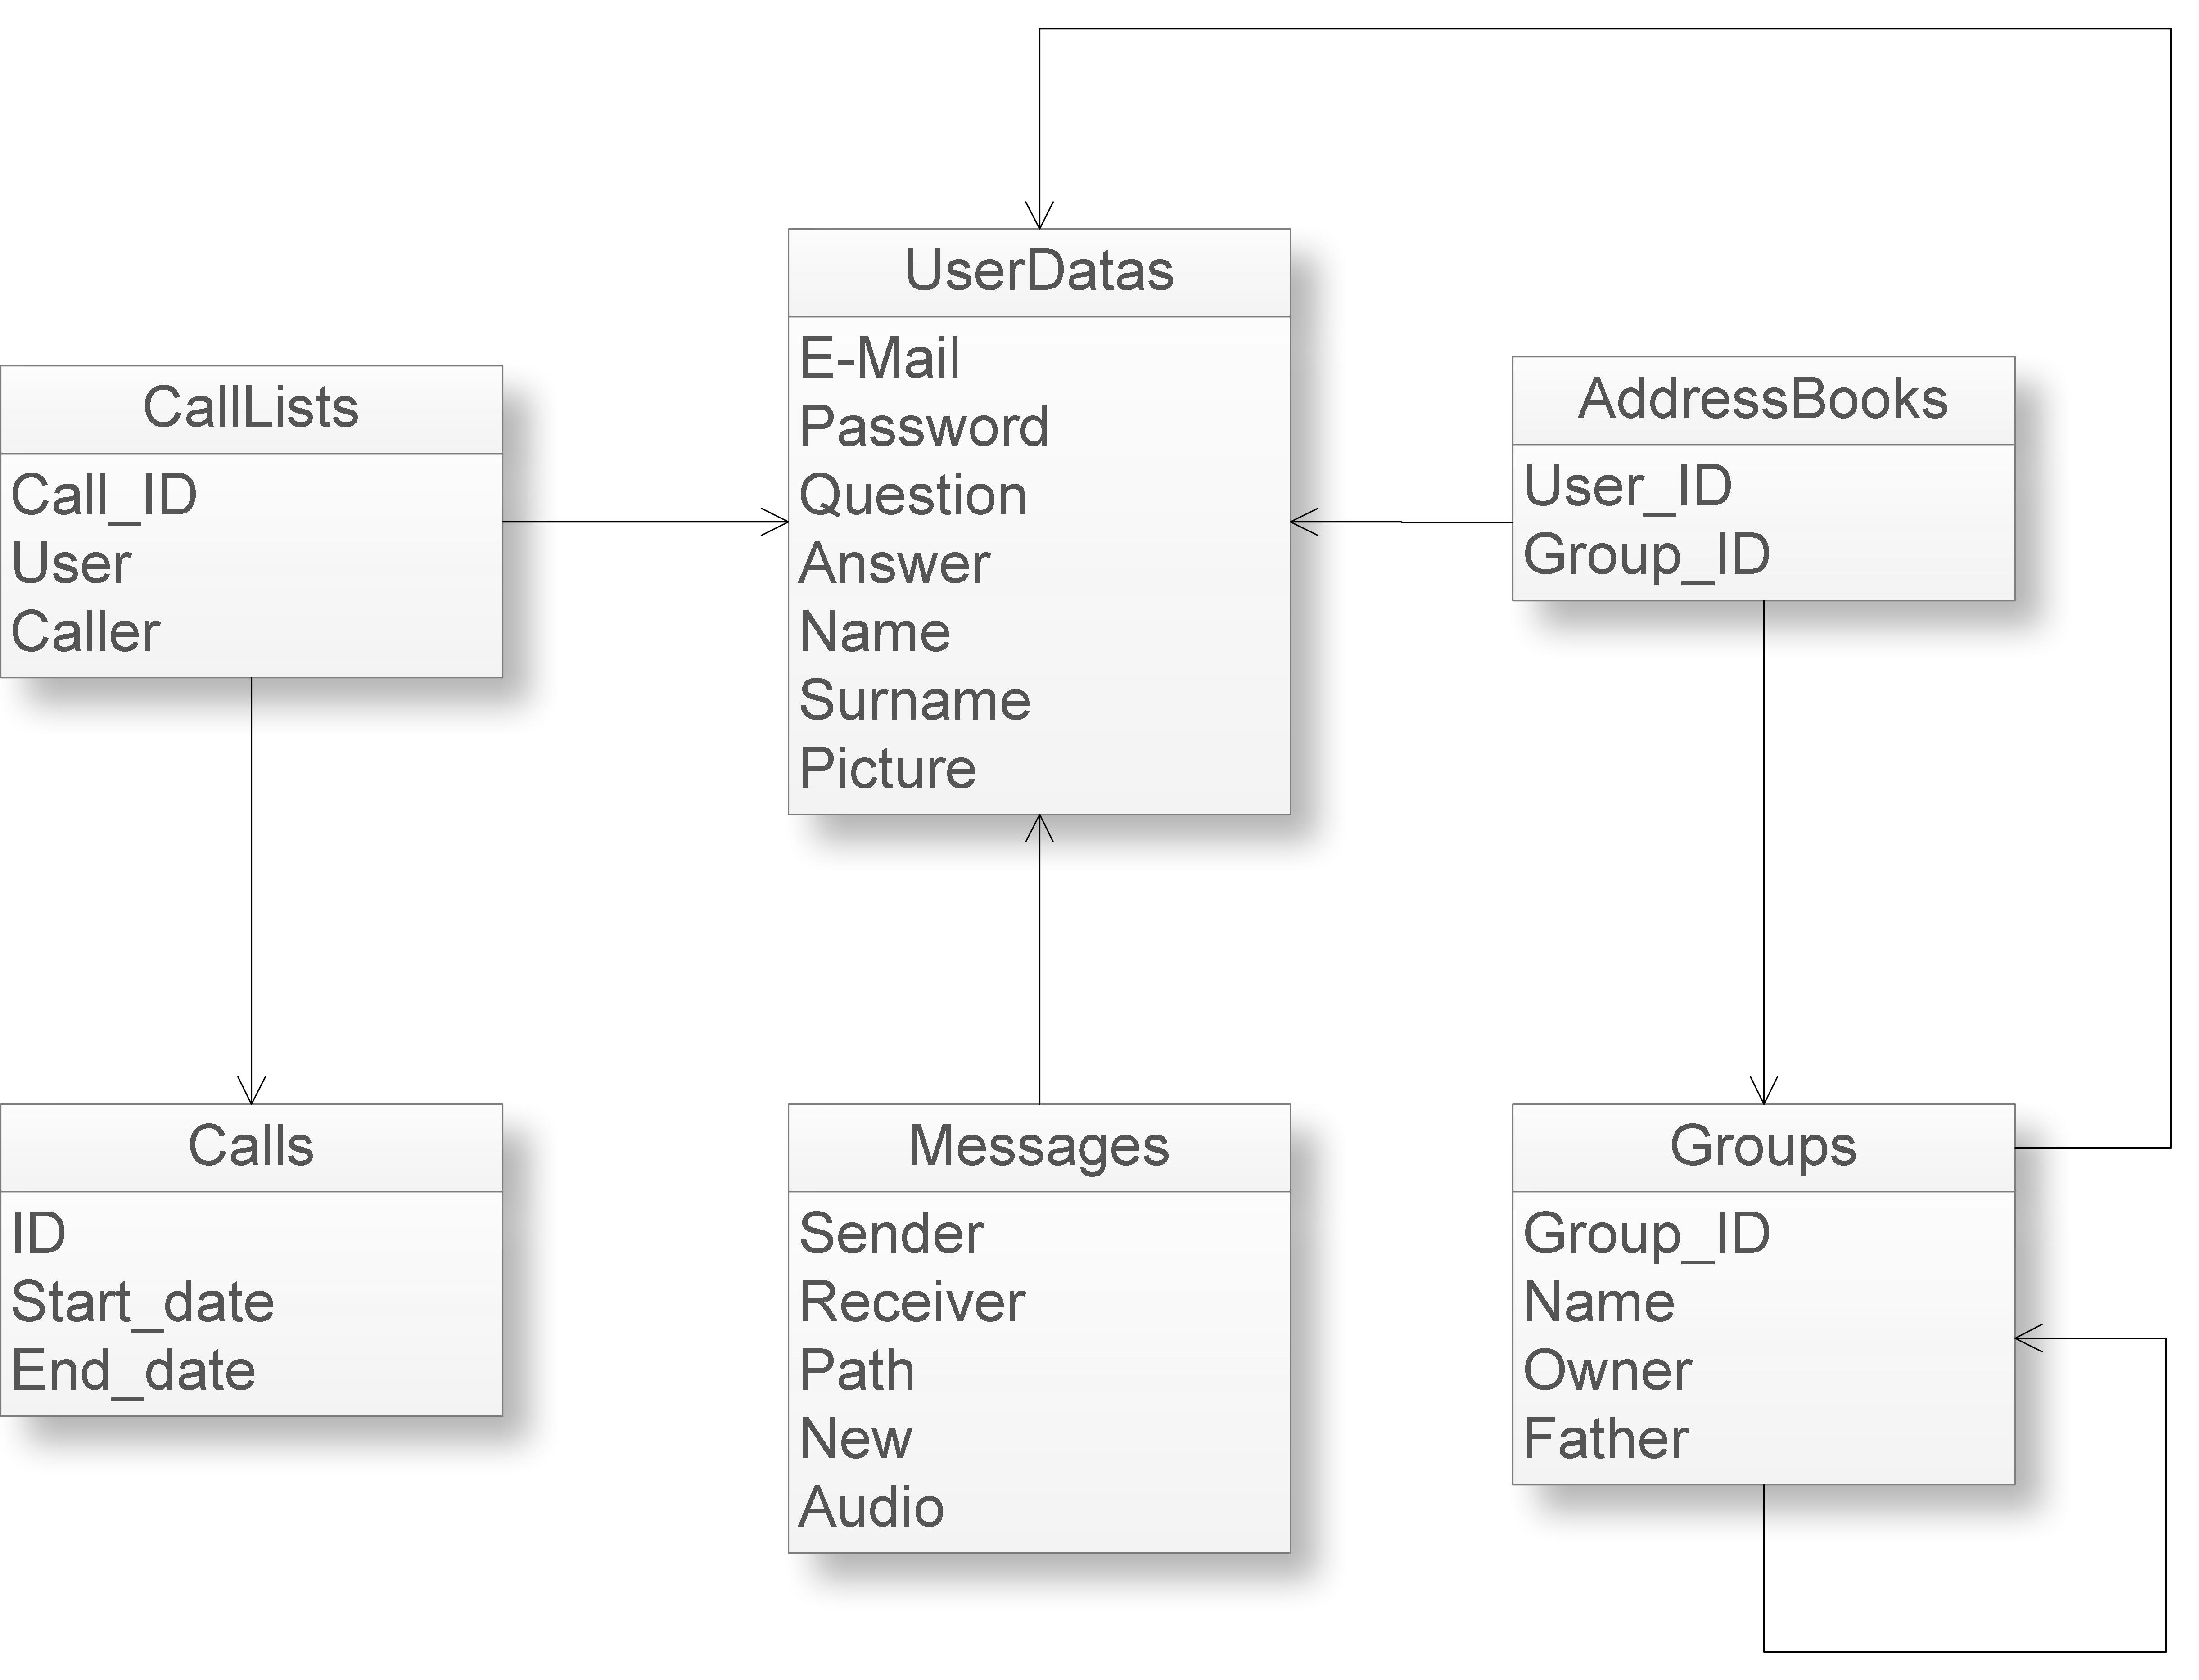
\includegraphics[width=.9\textwidth]{Database_logico}
\caption{Diagramma delle classi - Schema logico database}\label{fig:database_logico}
\end{center}
\end{figure}
\clearpage


\section{Architettura \texttt{mytalk.server}}\label{sec:server}
Tale sotto-architettura definisce le specifiche e le funzionalità dell'applicativo lato server. In esso saranno definiti i seguenti componenti:
\begin{itemize}[noitemsep,nolistsep]
	\item[-] \textsf{CS01 -- Gestione database};
	\item[-] \textsf{CS02 -- Gestione connessione};
	\item[-] \textsf{CS03 -- Gestione rubrica};
	\item[-] \textsf{CS04 -- Gestione autenticazione};
	\item[-] \textsf{CS05 -- Gestione segreteria};
	\item[-] \textsf{CS06 -- Gestione chiamate};
	\item[-] \textsf{CS07 -- Gestione controller}.
	\item[-] \textsf{CS08 -- Front controller}.
\end{itemize}

I componenti sopracitati verranno definiti rispettivamente nelle sottosezioni \ref{sec:cs01}, \ref{sec:cs02}, \ref{sec:cs03}, \ref{sec:cs04}, \ref{sec:cs05}, \ref{sec:cs06} e \ref{sec:cs07}. Si sottolinea sin da ora che il server è l'unico in grado di comunicare con il database su cui si poggia l'applicativo.

Infine si fa notare che i nomi di tutte le classi riportate nella presente sezione sono implicitamente parte del package \texttt{org.softwaresynthesis.mytalk.server}, pertanto tale prefisso sarà omesso nella loro denominazione.

%TODO Dio sia lodato, questa classe è stata salvata! SIA LODE E GLORIA AL SIGNORE!

\subsection{Componenti evidenziati}

\subsubsection{CS01 -- Gestione database}\label{sec:cs01}
\begin{description}
\item{\scshape\bfseries Descrizione:}\\
Tale componente si occupa di rappresentare la struttura del database relazionale su cui poggia l'applicativo, tramite esso il sistema potrà quindi effettuare operazione di lettura e scrittura di entità all'interno del database.

Nucleo logico del componente è la classe Singleton \texttt{SessionManager} (implementazione dell'interfaccia \texttt{ISession}), il cui compito è implementare una \inglese{factory} per le sessioni verso il database. Tali sessioni si basano sul file di configurazione di Hibernate, tra le cui informazioni compare anche la tipologia di DBMS utilizzata.

Hibernate necessita di definire una classe atta a rappresentare la struttura di un generico oggetto del database, essa è denominata \texttt{DataPersistanceManager}.
Per ogni oggetto del database così creato, sono predisposte delle operazioni per garantirne la modifica e permettere il ritorno dei dati in essi contenuti. Tali procedure sono descritte mediante  classi che implementano il \inglese{pattern} \inglese{template method}:

\begin{description}
\item[-] \texttt{GetUtil}: classe astratta che contiene i metodi per ottenere i valori dei campi dati intrinsechi dell'oggetto, essa viene quindi estesa da quattro sottoclassi: \texttt{GetCallUtil}, \texttt{GetGroupUtil}, \texttt{GetUserDataUtil} e \texttt{NotInitialize} ;
\item[-] \texttt{ModifyUtil}: una classe astratta che descrive una generica operazione di modifica ai campi dati dell'oggetto. Essa viene quindi estesa da tre sottoclassi: \texttt{DeleteUtil}, \texttt{UpdateUtil}, \texttt{InsertUtil}.
\end{description}

Il sistema definisce inoltre una classe \texttt{UtilFactory} usata per stabilire quale classe (tra quelle di \inglese{utility}) usare per l'esecuzione di un operazione su una tabella del database.

\texttt{DataPersistanceManager} ha la possibilità di creare (e usare) delle implementazioni dell'interfaccia \texttt{IMyTalkObject} che descrive il comportamento di un generico \textit{TrasferObject}.


Per chiarezza citiamo in tale sezione anche le classi che mappano le entità rappresentate nel database (implementazione di \texttt{IMyTalkObject}). Tali sono dotate di variabili di istanza che corrispondono ai campi dei \inglese{record}. Le operazioni disponibili su questo genere di oggetti comprendono i metodi \inglese{get}/\inglese{set} associati ai campi delle tabelle del database e sono rese disponibili dalle interfacce (una per ogni entità) implementate dalle classi.\footnote{%
	Per chiarezza, si precisa che tali classi corrispondono a quelle che nella logica di programmazione in Hibernate prendono il nome di \inglese{Transfer Object} (TO)\@.
	}
	\begin{itemize}
	  \item[-] \texttt{abook.IGroup}
	  \item[-] \texttt{abook.Group}
	  \item[-] \texttt{abook.IAddressBookEntry}
	  \item[-] \texttt{abook.AddressBookEntry}
	  \item[-] \texttt{abook.IUserData}
	  \item[-] \texttt{abook.UserData}
	  \item[-] \texttt{call.ICall}
	  \item[-] \texttt{call.Call}
	  \item[-] \texttt{call.ICallList}
	  \item[-] \texttt{call.CallList}
	  \item[-] \texttt{message.IMessage}
	  \item[-] \texttt{message.Message}
	\end{itemize}

Precisiamo che le classi rappresentanti i \inglese{transfer object} si trovano a essere collocate in package e componenti diversi da \texttt{server.dao}. Si è ritenuto infatti sensato inserire tali classi in contesti maggiormente specializzati, ad esempio la classe corrispondente ai messaggi in segreteria verrà ad essere collocata in \texttt{server.message}, mentre quella corrispondente alle chiamate in \texttt{server.call}.


\item{\scshape\bfseries Diagramma delle classi:}
\begin{figure}[H]
  \centering
  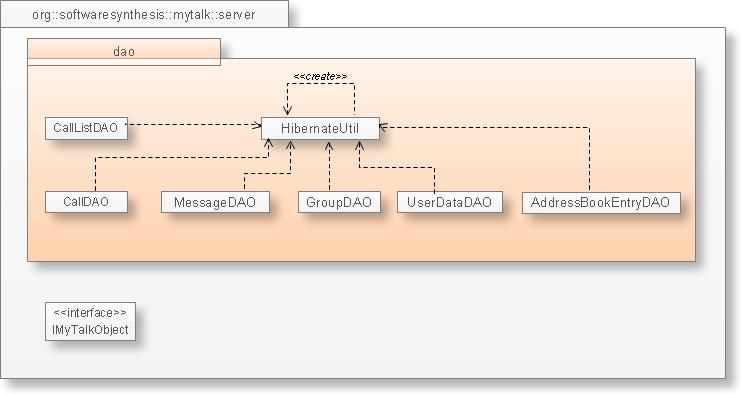
\includegraphics[width=.9\textwidth]{class_gestione_database}
  \caption{Diagramma delle classi - Gestione database}\label{fig:gestionedatabase}
\end{figure}

	\item{\scshape\bfseries Classi utilizzate:}
	\begin{itemize}[nolistsep, noitemsep]
	  \item[-] \texttt{server.dao.ISession}
	  \item[-] \texttt{server.dao.SessionManager}
	  \item[-] \texttt{server.dao.DataPersistanceManager}
	  \item[-] \texttt{server.dao.util.UtilFactory}
	  \item[-] \texttt{server.dao.util.GetUtil}
	  \item[-] \texttt{server.dao.util.GetCallUtil}
	  \item[-] \texttt{server.dao.util.GetGroupUtil}
	  \item[-] \texttt{server.dao.util.GetUserDataUtil}
	  \item[-] \texttt{server.dao.util.NotInitialize}
	  \item[-] \texttt{server.dao.util.ModifyUtil}
	  \item[-] \texttt{server.dao.util.DeleteUtil}
	  \item[-] \texttt{server.dao.util.UpdateUtil}
	  \item[-] \texttt{server.dao.util.InsertUtil}
	  \item[-] \texttt{server.IMyTalkObject}
	  
	\end{itemize}
\end{description}

\subsubsection{CS02 -- Gestione connessione}\label{sec:cs02}
\begin{description}
	\item{\scshape\bfseries Descrizione:}\\
Tale componente ingloba le classi destinate a stabilire le \inglese{routine} di connessione fra il server e i client del sistema, necessarie in un secondo momento a gestire le chiamate in ingresso e in uscita dai client.

La comunicazione bidirezionale fra il server e i client è ottenuta estendendo la classe fornita dalle librerie di \textit{TomCat} \texttt{org.apache.catalina.websocket.MessageInbound} mediante \texttt{connection.PushInbound}. In particolare sarà realizzato l'\inglese{overriding} del metodo \texttt{onTextMessage(CharBuffer)} in modo da permettere al componente \textsf{Gestione connessione} del server di reagire correttamente ai messaggi provenienti dal client in forma testuale.

Un ruolo essenziale è inoltre svolto dalla \inglese{servlet} \texttt{connection.ControllerManager}, realizzata estendendo mediante ereditarietà la classe fornita dalle librerie di \textit{Apache TomCat} \texttt{org.apache.catalina.websocket.WebSocketServlet}. Tale \inglese{servlet} non fa parte di questa componente, viene qui citata unicamente per chiarire l'interazione tra il client e il server in merito alla comunicazione. La \inglese{servlet} risiede, come si vedrà in seguito, nella componente \textsf{CS07 -- Gestione Controller}.

La caratteristica fondamentale della \inglese{servlet}, che rappresenta inoltre un punto di accesso centralizzato alle funzionalità del componente \textsf{Gestione connessione}, è quella di fare \inglese{overriding} del metodo \texttt{createWebSocketInbound(String, HttpServletRequest)} al fine di restituire un opportuno sottotipo di \texttt{org.apache.catalina.websocket.StreamInbound}. Il tipo dinamico dell'oggetto ritornato da \texttt{connection.ConnectionManager} corrisponde infatti proprio a \texttt{connection.PushInbound} in modo che lato client l'invocazione del costruttore di \texttt{WebSocket} (passando come parametro l'URL della \inglese{servlet}) crei una connessione del tipo voluto.

Ne consegue che, come sarà esposto con maggiori dettagli nella sezione \vref{sec:patternfactorymethod}, \texttt{createWebSocketInbound} è un'applicazione del \inglese{design pattern} Factory Method, in quanto la sottoclasse di \texttt{WebSocketServlet} restituisce un oggetto di tipo statico \texttt{StreamInbound} ma avente il tipo dinamico adatto agli scopi dell'applicazione.

	\item{\scshape\bfseries Diagramma delle classi:}
\begin{figure}[H]
  \centering
  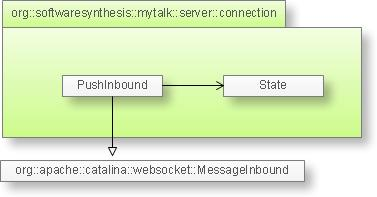
\includegraphics[width=.8\textwidth]{class_gestione_connessione}
  \caption{Diagramma delle classi - Gestione connessione}\label{fig:gestioneconnessione}
\end{figure}
	
	\item{\scshape\bfseries Classi utilizzate:}
	\begin{itemize}[nolistsep, noitemsep]
	  \item[-] \texttt{connection.PushInbound}
	  \item[-] \texttt{connection.State}
	  \item[-] \texttt{org.apache.catalina.websocket.MessageInbound}
	\end{itemize}
\end{description}

%TODO Dio sia lodato, questa classe è stata salvata! SIA LODE E GLORIA AL SIGNORE!

\subsubsection{CS03 -- Gestione rubrica}\label{sec:cs03}
\begin{description}
	\item{\scshape\bfseries Descrizione:}\\
A ogni utente del sistema, che corrisponde a un'istanza di \texttt{abook.UserData} (implementazione dell'interfaccia \texttt{abook.IUserData}), è associata una rubrica personale. 

La rubrica è rappresentata da una lista di \texttt{abook.IAddressBookEntry}, per la quale si fornisce un'implementazione nominata \texttt{abook.AddressBookEntry} che rappresenta un contatto della rubrica di un utente. Come si evince dal diagramma riportato in figura \ref{fig:gestionerubrica}, la struttura del componente rispecchia la logica di funzionamento del database.

Di conseguenza ogni istanza di tipo \texttt{abook.AddressBookEntry} apparterrà a un solo \texttt{abook.IUserData} e in essa è registrata un'istanza di \texttt{abook.UserData} che rappresenta il contatto facente parte della rubrica.

Gli utenti inoltre possono essere opzionalmente organizzati in gruppi: un contatto in rubrica può, in un dato momento, appartenere a uno o più gruppi oppure non appartenere a nessuno. Per tale motivo ogni istanza di \texttt{abook.AddressBookEntry} contiene anche un riferimento di tipo \texttt{IGroup}.

Tale interfaccia, congiuntamente alla sua implementazione \texttt{abook.Group}, permettono di rappresentare i gruppi della rubrica di un utente.

Infine sono stati predisposti 12 \inglese{controller} per interagire con le classi di questa componente:

\begin{itemize}
	  \item \texttt{abook.controller.AddContactController}
	  \item \texttt{abook.controller.DeleteContactController}
	  \item \texttt{abook.controller.AddGroupController}
	  \item \texttt{abook.controller.DeleteGroupController}
	  \item \texttt{abook.controller.AddInGroupController}
	  \item \texttt{abook.controller.RemoveFromGroupController}
	  \item \texttt{abook.controller.BlockContactController}
	  \item \texttt{abook.controller.UnblockContactController}
	  \item \texttt{abook.controller.GetContactsController}
	  \item \texttt{abook.controller.GetGroupsController}
	  \item \texttt{abook.controller.SearchController}
	  \item \texttt{abook.controller.AccountSettingsController}
\end{itemize}

Le loro funzionalità riguardano principalmente le possibilità di modificare, creare e cancellare istanze di oggetti del tipo \texttt{transfer object} e quindi riconducibili ad oggetti fisicamente presenti nel database. I \inglese{controller} saranno descritte con maggiori dettaglio nella sezione \vref{sec:cs07} (\textsf{CS07 -- Gestione controller}).

	\item{\scshape\bfseries Diagramma delle classi:}
\begin{figure}[H]
  \centering
  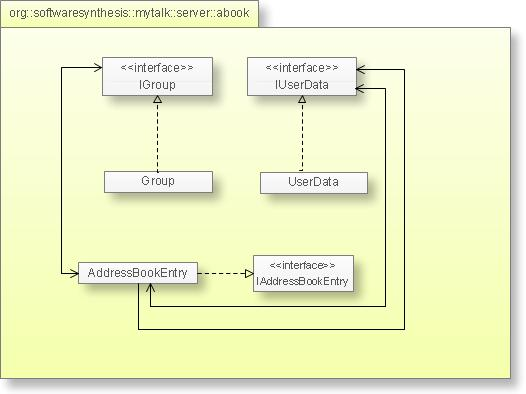
\includegraphics[width=.7\textwidth]{class_gestione_rubrica}
  \caption{Diagramma delle classi - Gestione rubrica}\label{fig:gestionerubrica}
\end{figure}
	
	\item{\scshape\bfseries Classi utilizzate:}\\
	\begin{itemize}[nolistsep, noitemsep]
	  \item[-] \texttt{abook.AddressBookEntry}
	  \item[-] \texttt{abook.IAddressBookEntry}
	  \item[-] \texttt{abook.IGroup}
	  \item[-] \texttt{abook.Group}
	  \item[-] \texttt{abook.IUserData}
	  \item[-] \texttt{abook.UserData}
	\end{itemize}
\end{description}

%TODO Dio sia lodato, questa classe è stata salvata! SIA LODE E GLORIA AL SIGNORE!

\subsubsection{CS04 -- Gestione autenticazione}\label{sec:cs04}
\begin{description}
  \item{\scshape\bfseries Descrizione:}\\
L'autenticazione passa attraverso due fasi: la richiesta di \inglese{login} e l'approvazione (\inglese{commit}). La richiesta di \inglese{login} verifica le credenziali di accesso con i dati memorizzati all'interno del database, mentre la richiesta di \inglese{commit} assegna al \inglese{subject} che ha attivato la procedura di autenticazione, dei valori identificativi che permettano di identificarlo finché esso utilizza il sistema software.

Quando un utente avvia la procedura di autenticazione il controller che espone le funzionalità di questo componente, \texttt{authentication.controller.LoginController} crea il contesto di autenticazione generando un istanza di \texttt{authentication.CredentialLoader} che ha il compito di caricare le credenziali di accesso (caricando i dati di autenticazione mediante \texttt{authentication.NameLoader} e \texttt{authentication.PasswordLoader}) e accede al file di configurazione per istanziare il giusto modulo per l'autenticazione, costituito dalla classe \texttt{authentication.AuthenticationModule}.

La componente predispone anche le funzionalità da usare per eseguire il \inglese{logout} di un utente registrato nel sistema, e la registrazione al sistema stesso. Tale funzionalità saranno richiamabili mediante 2 controller:
\begin{itemize}
	\item \texttt{authentication.controller.LogoutController}
	\item \texttt{authentication.controller.RegisterController}
\end{itemize}

Altri due controller sono predisposti per il recupero della password. Nello specifico: 

\begin{itemize}
	\item \texttt{authentication.controller.QuestionController}: per richiedere al server la domanda segreta a cui rispondere.
	\item \texttt{authentication.controller.AnswerController} per richiedere al server la validazione della risposta inserita dall'utente.
\end{itemize}

Per garantire un buon livello di sicurezza nell'invio dei dati l'applicativo si appoggia ad un sistema di criptazione basato su algoritmo AES. La classe che fornisce tali funzionalità è \texttt{authentication.security.AESAlgorithm}, implementazione di \texttt{authentication.security.ISecurityStrategy}. Tale classe fornisce due procedure, quella per criptare i dati e quella per decriptarli. Esse sono rappresentate dalle classi \texttt{authentication.security.AESEncode} e \texttt{authentication.security.AESDecode}. Entrambe estendono la classe astratta \texttt{authentication.security.AESTemplate} e basano la propria implementazione sul \inglese{pattern} \texttt{Template Method}.
  
  \item{\scshape\bfseries Diagramma delle classi:}
\begin{figure}[H]
  \centering
%TODO questo diagramma manca
 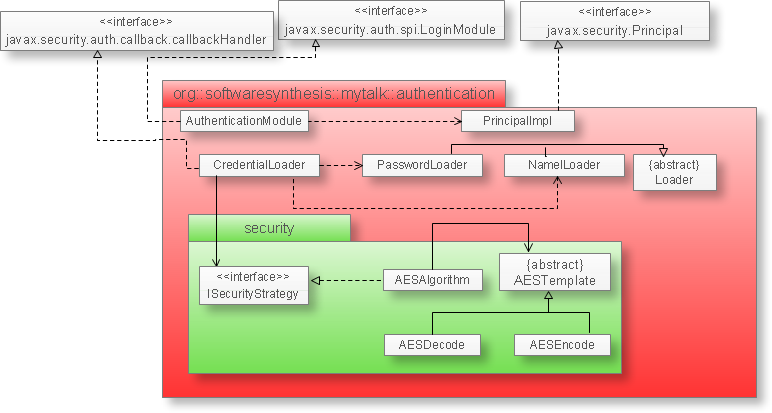
\includegraphics[width=.8\textwidth]{class_gestione_autenticazione}
  \caption{Diagramma delle classi - Gestione autenticazione}\label{fig:gestioneautenticazione}
\end{figure}	
  
  \item{\scshape\bfseries Classi utilizzate}
  \begin{itemize}
    \item[-] \texttt{authentication.AuthenticationModule}
	\item[-] \texttt{authentication.CredentialLoader}
	\item[-] \texttt{authentication.PrincipalImpl}
	\item[-] \texttt{authentication.Loader}
	\item[-] \texttt{authentication.NameLoader}
	\item[-] \texttt{authentication.PasswordLoader}
	\item[-] \texttt{authentication.security.ISecurityStrategy}
 	\item[-] \texttt{authentication.security.AESAlgorithm}
 	\item[-] \texttt{authentication.security.AESTemplate}
 	\item[-] \texttt{authentication.security.AESEncode}
 	\item[-] \texttt{authentication.security.AESDecode}	
 	\item[-] \texttt{javax.security.auth.spi.LoginModule}
 	\item[-] \texttt{javax.security.auth.callback.CallbackHandler}
 	\item[-] \texttt{javax.security.Principal}
  \end{itemize}

\end{description}

%TODO Dio sia lodato, questa classe è stata salvata! SIA LODE E GLORIA AL SIGNORE!

\subsubsection{CS05 -- Gestione segreteria}\label{sec:cs05}
\begin{description}
	\item{\scshape\bfseries Descrizione:}\\
I messaggi in segreteria, che possono essere di natura audio o audio/video, corrispondono alle istanze dalla classe \texttt{message.Message} (implementazione dell'interfaccia \texttt{message.IMessage}) e sono caratterizzati da un utente mittente, da un destinatario e dalla data di registrazione.

La collezione di messaggi aventi un determinato utente come destinatario può essere ottenuta tramite un'operazione dichiarata nell'interfaccia \texttt{abook.IUserData}.

Per consentire ai client di accedere alle funzionalità gestite da questo componente sono state predisposte dei \inglese{controller} e saranno descritti con maggiori dettagli nella sezione \vref{sec:cs07}. Al fine di comunicare le funzionalità proposte viene di seguito riportata la lista dei \inglese{controller} che comunicano con tale componente:

\begin{itemize}
	\item \texttt{message.controller.AddMessageController}: viene utilizzata da un client \textit{A} per lasciare un messaggio nella segreteria di un client \textit{B};
	\item \texttt{message.controller.DeleteMessageController}: viene utilizzata da un client per rimuovere un messaggio presente nella propria segreteria;
	\item \texttt{message.controller.UpdateMessageController}: viene utilizzata per modificare lo stato di un messaggio da ``da leggere'' a ``letto'';
	\item \texttt{message.controller.GetMessagesController}: viene utilizzata da un client per scaricare la lista dei messaggi presenti nella sua segreteria;
\end{itemize}

	\item{\scshape\bfseries Diagramma delle classi:}
\begin{figure}[H]
  \centering
  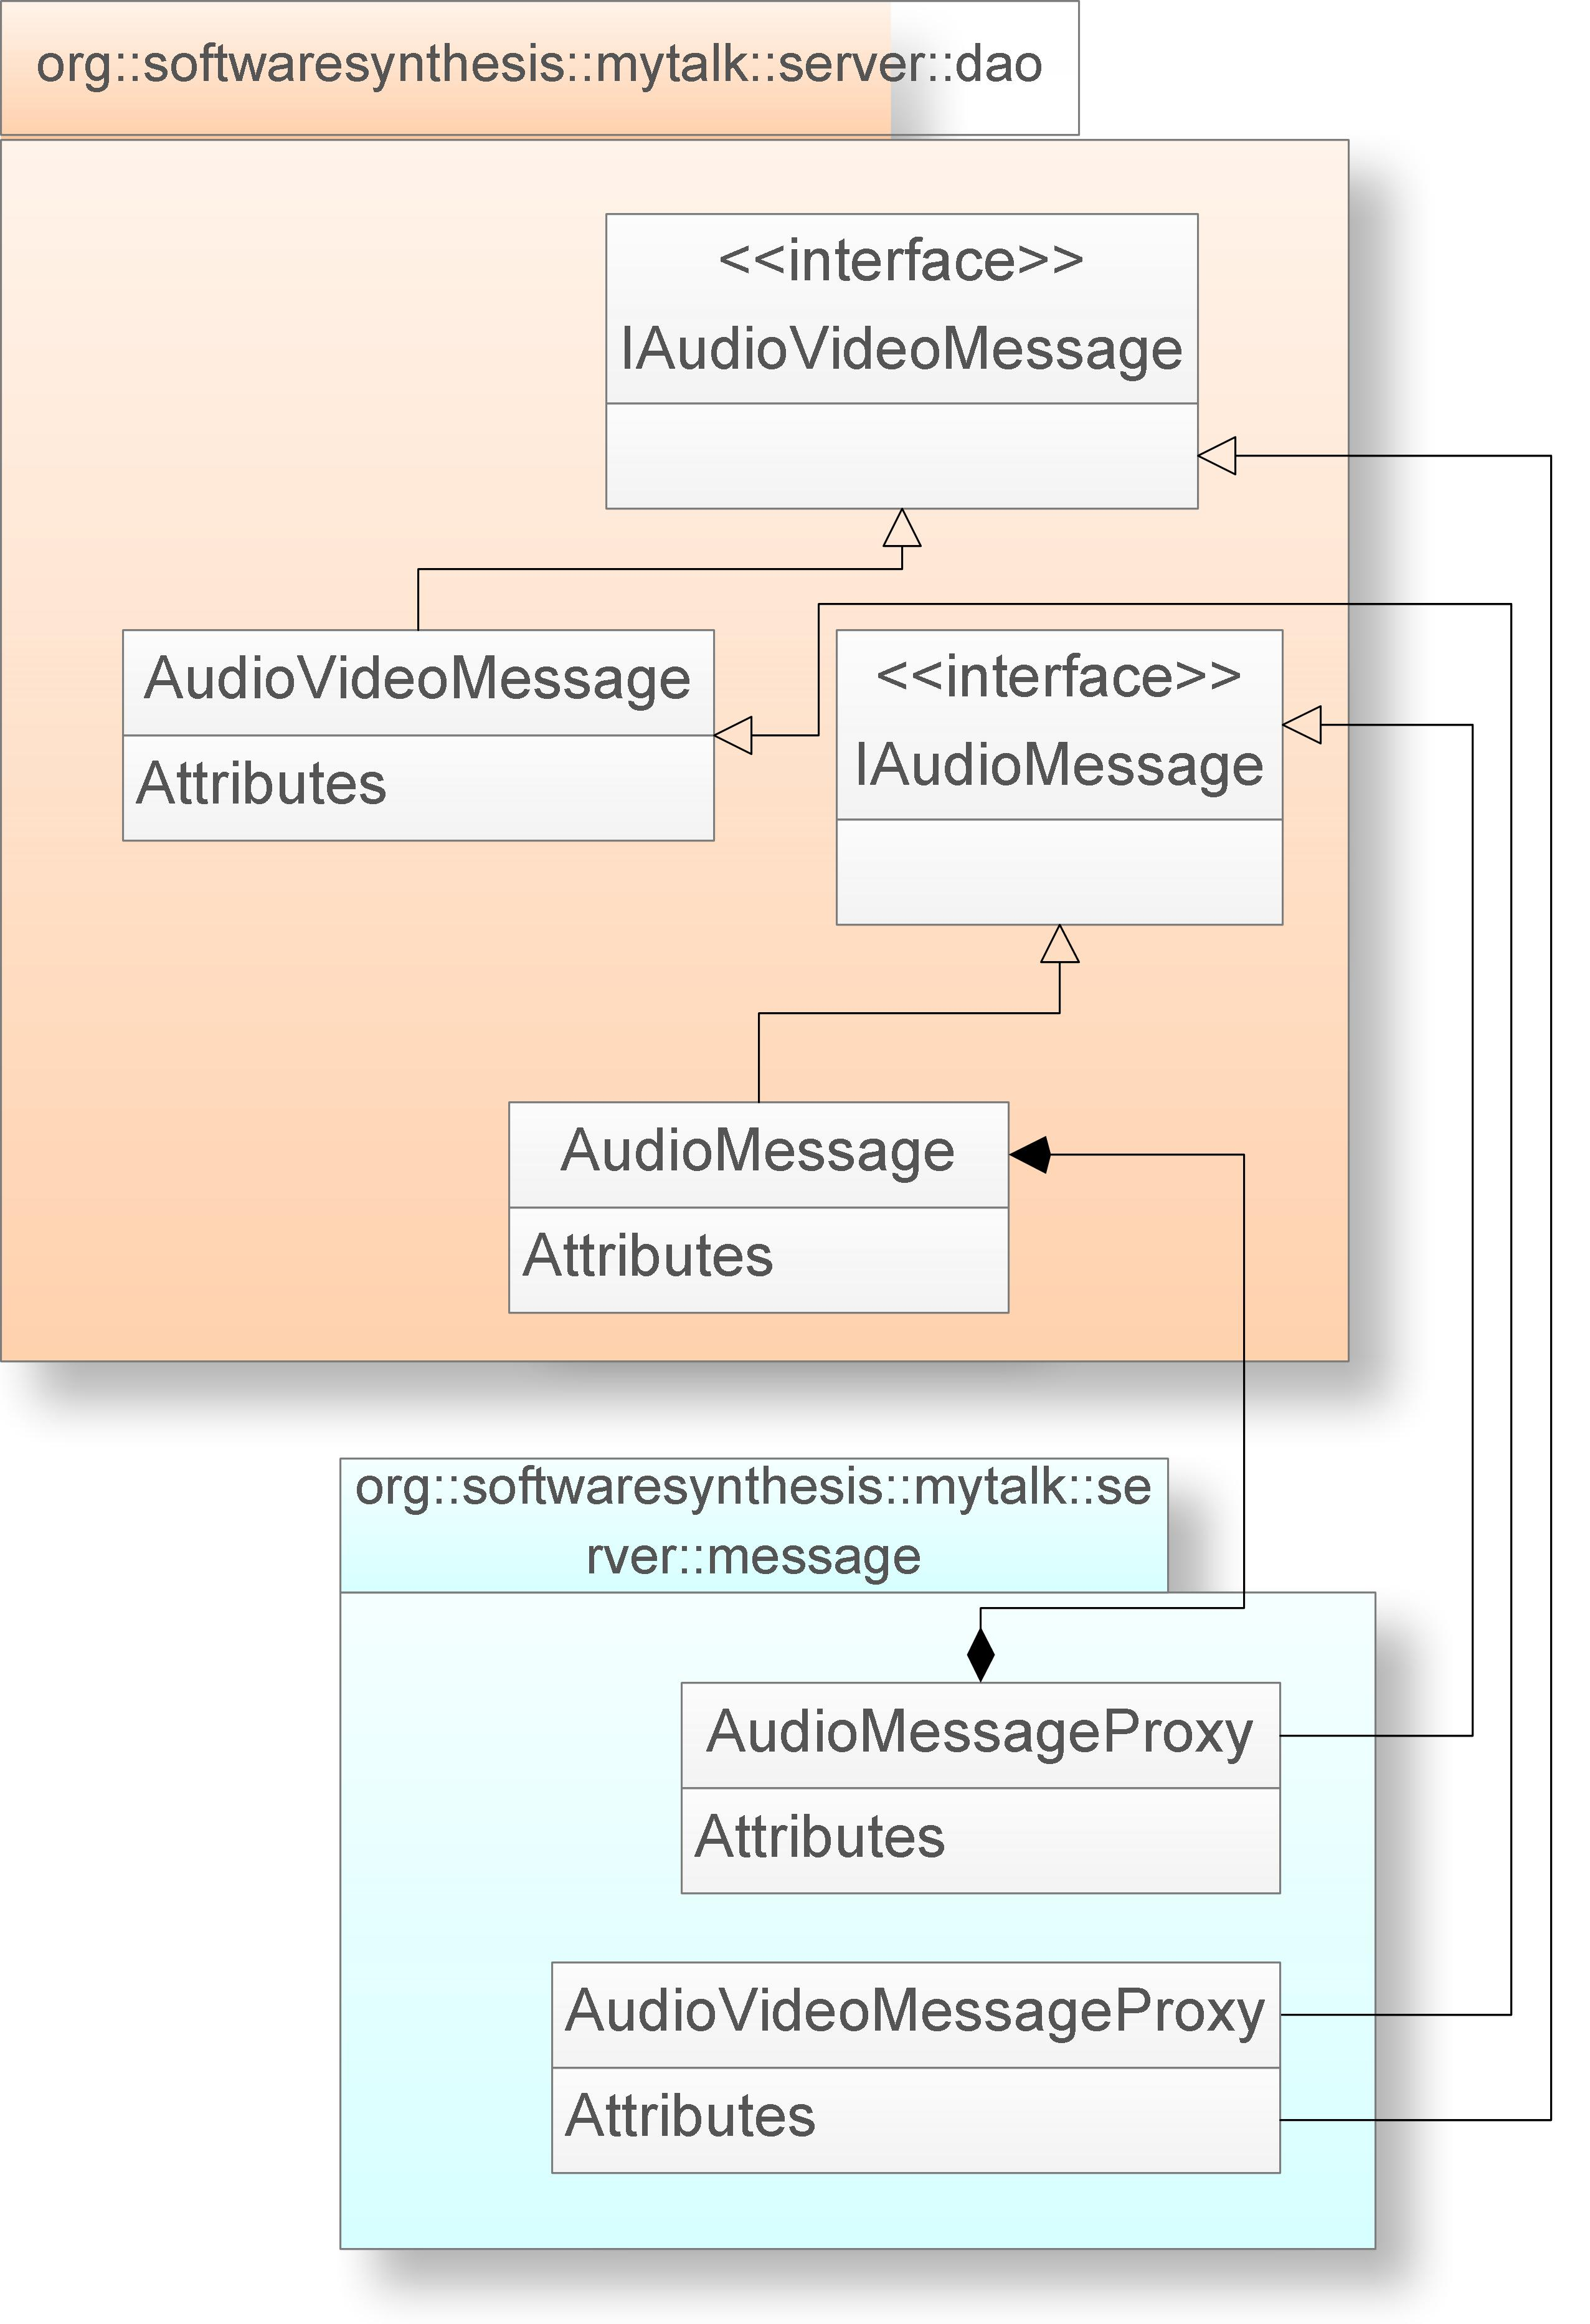
\includegraphics[width=.8\textwidth]{class_gestione_segreteria}
  \caption{Diagramma delle classi - Gestione segreteria}\label{fig:gestionesegreteria}
\end{figure}	
	
	\item{\scshape\bfseries Classi utilizzate:}
	\begin{itemize}[noitemsep,nolistsep]
		\item[-] \texttt{message.IMessage}
	  	\item[-] \texttt{message.Message}
	\end{itemize}
\end{description}

%TODO Dio sia lodato, questa classe è stata salvata! SIA LODE E GLORIA AL SIGNORE!

\subsubsection{CS06 -- Gestione chiamate}\label{sec:cs06}
\begin{description}
  \item{\scshape\bfseries Descrizione:}\\
Le classi di questo componente hanno il ruolo di definire una strutturata per definire lo storico delle chiamate di un utente e, conseguentemente, l'accesso ai dati relativi a una chiamata (data, mittente e $n\geq1$ destinatari della chiamata).

La componente contiene l'interfaccia \texttt{ICall} e la sua implementazione lato server \texttt{Call}, che rappresenta il \inglese{transfer object} per la rappresentazione della chiamata che deve essere mappata nel database. Ogni chiamata \texttt{ICall} è associata ad un istanza di un oggetto implementante \texttt{ICallList}. Nel nostro caso tale oggetto sarà un istanza di \texttt{CallList}.

Infine, allo scopo di consentire ai client l'accesso alle funzionalità di questo componente, è stata prevista un \inglese{controller} \texttt{call.controller.GetCallsController} il cui ruolo sarà descritto con maggiori dettagli nella sezione \vref{sec:cs07}.

  \item{\scshape\bfseries Diagramma delle classi:}
\begin{figure}[H]
  \centering
  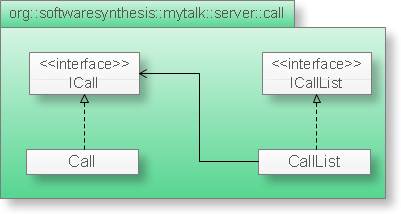
\includegraphics[width=.6\textwidth]{class_gestione_chiamate}
  \caption{Diagramma delle classi - Gestione chiamate}\label{fig:gestionechiamate}
\end{figure}

  \item{\scshape\bfseries Classi utilizzate:}\\
  \begin{itemize}[noitemsep,nolistsep]
    \item[-] \texttt{call.ICall}
    \item[-] \texttt{call.Call}
    \item[-] \texttt{call.ICallList}
    \item[-] \texttt{call.CallList}
  \end{itemize}
\end{description}

%TODO Dio sia lodato, questa classe è stata salvata! SIA LODE E GLORIA AL SIGNORE!

\subsubsection{CS07 -- Gestione Controller}\label{sec:cs07}
\begin{description}
	\item{\scshape\bfseries Descrizione:}\\
Il componente ha il ruolo di descrivere tutte le funzionalità che il sistema server è in grado di svolgere, ad esempio il blocco di un contatto, l'aggiunta dello stesso alla rubrica, ad un gruppo, o la ricerca di uno specifico nel database generale. A tali funzionalità si accede mediante un front controller (CS08, descritto nel paragrafo successivo) che implementa un sistema che permette di monitorare le richieste sulle stesse.

Per ogni operazione viene definito un controller (classe che estende \texttt{AbstracController}, un implementazione di \texttt{IController}). La mappatura fra componenti del server e i rispettivi \inglese{controller} è illustrata dalla seguente tabella:

\begin{center}
\rowcolors{2}{lightblue}{llightblue}
\begin{tabular}{>{\sffamily}l>{\ttfamily}p{.6\textwidth}}
\toprule
\textbf{\rmfamily Componente} & \textbf{\rmfamily Controller}\\
\midrule
CS03 -- Gestione rubrica 


& abook.controller.AddContactController\\
& abook.controller.DeleteContactController\\
& abook.controller.AddGroupController\\
& abook.controller.DeleteGroupController\\
& abook.controller.AddInGroupController\\
& abook.controller.DeleteFromGroupController\\
& abook.controller.BlockContactController\\
& abook.controller.UnblockContactController\\
& abook.controller.GetContactsController\\
& abook.controller.GetGroupsController\\
& abook.controller.SearchController\\
& abook.controller.AccountSettingsController\\


CS04 -- Gestione autenticazione 


& authentication.controller.LoginController\\
& authentication.controller.LogoutController\\
& authentication.controller.RegisterController\\
& authentication.controller.QuestionController\\
& authentication.controller.AnswerController\\



CS05 -- Gestione segreteria 

& message.controller.AddMessageController\\
& message.controller.DeleteMessageController\\
& message.controller.UpdateMessageController\\
& message.controller.GetMessagesController\\



CS06 -- Gestione chiamate 

& call.controller.GetCallsController\\
& call.controller.AddCallController\\

\bottomrule
\end{tabular}
\end{center}

Il compito di interfacciarsi con \textsf{Gestione rubrica} per recuperare la rubrica associata ad un utente e per riflettere sul server le operazioni di amministrazione della rubrica spetta invece al pacchetto di \inglese{controller} \texttt{abook.controller}. Tali \inglese{controller} rispondono anche alle richieste dei client per le azioni di aggiornamento e modifica dell'account personale dell'utente associato al client. Nello specifico si ha:

\begin{itemize}
	  \item[-] \texttt{abook.controller.AddContactController}: richiamata dal front controller per aggiungere un contatto alla propria rubrica utente;
	  \item[-] \texttt{abook.controller.DeleteContactController}: richiamata dal front controller per rimuovere un contatto dalla propria rubrica;
	  \item[-] \texttt{abook.controller.AddGroupController}: richiamata dal front controller per creare un nuovo gruppo contatti;
	  \item[-] \texttt{abook.controller.DeleteGroupController}: richiamata dal front controller per eliminare un gruppo;
	  \item[-] \texttt{abook.controller.AddInGroupController}: richiamata dal front controller, su richiesta di un client, per inserire un contatto in un gruppo;
	  \item[-] \texttt{abook.controller.DeleteInGroupController}: richiamata dal front controller, su richiesta di un client, per rimuovere un contatto da un gruppo della propria rubrica;
	  \item[-] \texttt{abook.controller.BlockContactController}: richiamata dal front controller, su richiesta di un client, per bloccare un contatto presente nella propria rubrica, indifferentemente dai gruppi (della rubrica del client) in cui esso si trova;
	  \item[-] \texttt{abook.controller.UnblockContactController}: richiamata dal front controller, su richiesta di un client, per sbloccare un contatto presente nella propria rubrica;
	  \item[-] \texttt{abook.controller.GetContactsController}: richiamata dal front controller, su richiesta di un client, per scaricare la lista dei contatti presenti nella propria rubrica;
	  \item[-] \texttt{abook.controller.GetGroupsController}: richiamata dal front controller (su richiesta di un client) per scaricare lista dei contatti e dei gruppi in cui in cui il richiedente è inserito;
	  \item[-] \texttt{abook.controller.SearchController}: utilizzata per ricercare gli utente contenenti nei parametri nome, cognome o mail, una parola chiave usata per fare la ricerca e passata al \inglese{controller};
	  \item[-] \texttt{abook.controller.AccountSettingsController}: richiamata dal front controller per modificare i dati del client nel server.
\end{itemize}

I cambiamenti di stato di un utente sono invece processati da \texttt{Controller Manager} che fornisce di conseguenza anch'esso un punto d'accesso al componente \textsf{Gestione rubrica}.

Ai fini del \inglese{login} è utilizzato invece il \inglese{controller} \texttt{authentication.controller.LoginController}, che ha il compito di interfacciarsi con il sistema di autenticazione e, in particolare, con l'istanza del sottotipo di \texttt{javax.security.auth.spi.LoginModule} in uso per verificare le credenziali. Inoltre come già accennato sono presenti il \inglese{controller} per il \inglese{logout} \texttt{authentication.controller.LogoutController}, quello per la registrazione al sistema \texttt{authentication.controller.RegisterController} e quelli per la domanda segreta e la risposta alla medesima, rispettivamente \texttt{authentication.controller.QuestionController} e \texttt{authentication.controller.AnswerController}.\\

Infine il download e la gestione della segreteria telefonica (di competenza di \textsf{Gestione segreteria}) e dello storico delle chiamate (per quanto riguarda il componente \textsf{Gestione chiamate}) avvengono in risposta alle richieste dei client pervenute al pacchetto di controller \texttt{message.controller} e \texttt{call.controller.GetCallsController} rispettivamente. 

	\item{\scshape\bfseries Diagramma delle classi:}
\begin{figure}[H]
  \centering
  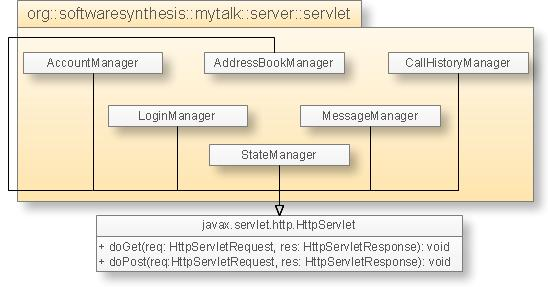
\includegraphics[width=.7\textwidth]{class_facade_server}
  \caption{Diagramma delle classi - Gestione controller}\label{fig:facadeserver}
\end{figure}

Il diagramma in figura \ref{fig:facadeserver} rappresenta la gerarchia dei \inglese{controller} del front controller ma non mostra in dettaglio le dipendenze fra ognuna di questi e i componenti interni ai sotto-package \texttt{abook}, \texttt{authentication}, \texttt{call}, \texttt{connection} e \texttt{message} per non appesantire troppo la notazione.

Tali dipendenze, di fondamentale importanza per l'architettura, sono però riportate nei diagrammi della sezione \vref{sec:patternfacade} in cui è descritta con maggiori dettagli l'applicazione del \inglese{design pattern} front controller.
	
	\item{\scshape\bfseries Classi utilizzate:}\\
	\begin{itemize}[noitemsep,nolistsep]
	  \item[-] \texttt{IController}
	  \item[-] \texttt{AbstractController}
	  \item[-] \texttt{connection.ChannelServlet}
	  \item[-] \texttt{abook.controller.AddContactController}
	  \item[-] \texttt{abook.controller.DeleteContactController}
	  \item[-] \texttt{abook.controller.AddGroupController}
	  \item[-] \texttt{abook.controller.DeleteGroupController}
	  \item[-] \texttt{abook.controller.AddInGroupController}
	  \item[-] \texttt{abook.controller.RemoveFromGroupController}
	  \item[-] \texttt{abook.controller.BlockContactController}
	  \item[-] \texttt{abook.controller.UnblockContactController}
	  \item[-] \texttt{abook.controller.GetContactsController}
	  \item[-] \texttt{abook.controller.GetGroupsController}
	  \item[-] \texttt{abook.controller.SearchController}
	  \item[-] \texttt{abook.controller.AccountSettingsController}	  
	  \item[-] \texttt{authentication.controller.LoginController}
	  \item[-] \texttt{authentication.controller.LogoutController}
	  \item[-] \texttt{authentication.controller.RegisterController}
	  \item[-] \texttt{authentication.controller.QuestionController}
	  \item[-] \texttt{authentication.controller.AnswerController}
	  \item[-] \texttt{message.controller.AddMessageController}
	  \item[-] \texttt{message.controller.DeleteMessageController}
	  \item[-] \texttt{message.controller.UpdateMessageController}
	  \item[-] \texttt{message.controller.GetMessagesController}
	  \item[-] \texttt{call.controller.GetCallsController}
	  \item[-] \texttt{call.controller.AddCallController}
	  \item[-] \texttt{javax.servlet.http.HttpServlet}
	  \item[-] \texttt{org.apache.catalina.websocket.WebSocketServlet}
	\end{itemize}
\end{description}

\subsubsection{CS08 -- Front controller}
\begin{description}
	\item{\scshape\bfseries Descrizione:}\\
Tale componente ha il ruolo di offrire ai client un punto di accesso alle funzionalità del sistema server descritte nel paragrafo precedente. Dal momento che tale interazione avviene in un contesto distribuito, il punto di accesso ai componenti del server è stato implementato come una \inglese{servlet} Java destinata ad essere eseguita nell'ambiente del \inglese{servlet container} fornito da \textit{Apache TomCat}.

La classe Java \texttt{HttpServlet} implementa un sistema di \inglese{listening} che permette di monitorare costantemente richieste in ingresso. Queste ultime possono essere di duplice natura e corrispondono ai metodi di invio dei dati previsti dal protocollo HTTP (\texttt{GET} e \texttt{POST}).

Per riconoscere il tipo di richiesta inoltrata il \inglese{front controller}, rappresentato dalla classe \texttt{ControllerManager}, si appoggia ad un \inglese{file .properties} contenente le associazioni tra i nomi dei controller e i percorsi delle classi corrispondenti.

	\item{\scshape\bfseries Diagramma delle classi:}\\
%TODO: INSERIRE DIAGRAMMA CLASSI FRONT CONTROLLER

Il diagramma in figura X rappresenta l'implementazione generica del \inglese{front controller} che, come anticipato, nasconde agli utilizzatori l'iter per la gestione dei specifici servizi (rubrica, segreteria, autenticazione, etc.). Per ogni servizio è descritta con maggiori dettagli e la relativa rappresentazione grafica, l'applicazione del \inglese{design pattern} nel paragrafo \vref{sec:patternfacade}.

\item{\scshape\bfseries Classi utilizzate:}\\
	\begin{itemize}[noitemsep,nolistsep]
	  \item[-] \texttt{ControllerManager}
	\end{itemize}

\end{description}
\subsection{Descrizione delle classi}

\subsubsection{Package \texttt{org.softwaresynthesis.mytalk.server}}

\begin{itemize}[leftmargin=0em]

\item \texttt{IController}
\begin{description}
  \item{\scshape\bfseries Descrizione:}\\
Interfaccia che definisce un generico controller.
  \item{\scshape\bfseries Componenti che ne fanno uso:}
  \begin{itemize}[noitemsep,nolistsep]
    \item[-] \textsf{CS07 -- Gestione controller}
    \item[-] \textsf{CS08 -- Front controller}
  \end{itemize}
\end{description}

\item \texttt{AbstractController}
\begin{description}
  \item{\scshape\bfseries Descrizione:}\\
Classe astratta che implementa \texttt{IController}. Fornisce un implementazione di base di un controller generico.
  \item{\scshape\bfseries Componenti che ne fanno uso:}
  \begin{itemize}[noitemsep,nolistsep]
    \item[-] \textsf{CS07 -- Gestione controller}
    \item[-] \textsf{CS08 -- Front controller}
  \end{itemize}
\end{description}

\item \texttt{ControllerManager}
\begin{description}
  \item{\scshape\bfseries Descrizione:}\\
Classe che costituisce il front controller del server. Ogni richiesta inoltrata al server dovrà passare per questa classe. Essa avrà quindi il compito di riconoscere il tipo di richiesta (tramite un associazione nomi richiesta - classe destinataria), e di creare quindi un istanza del controller associato.
  \item{\scshape\bfseries Componenti che ne fanno uso:}
  \begin{itemize}[noitemsep,nolistsep]
    \item[-] \textsf{CS08 -- Front controller}
  \end{itemize}
\end{description}

\end{itemize}

\subsubsection{Package \texttt{org.softwaresynthesis.mytalk.server.dao}}

\begin{itemize}[leftmargin=0em]

\item \texttt{ISession}
\begin{description}
  \item{\scshape\bfseries Descrizione:}\\
Interfaccia che definisce un generico componente che gestisce una sessione Hibernate.
  \item{\scshape\bfseries Componenti che ne fanno uso:}
  \begin{itemize}[noitemsep,nolistsep]
    \item[-] \textsf{CS01 -- Gestione database}
    \item[-] \textsf{CS07 -- Gestione controller}
  \end{itemize}
\end{description}

\item \texttt{DataPersistanceManager}
\begin{description}
  \item{\scshape\bfseries Descrizione:}\\
Classe che rappresenta una generica istanza di una tabella del database gestito mediante Hibernate, la classe contiene associazioni:
\begin{itemize}
\item alla sessione Hibernate in corso (riferimento ad un oggetto \texttt{ISession});
\item alla classe che definisce le operazioni di get (\texttt{GetUtil)};
\item alla classe che definisce le operazioni di modifica ai campi membro dell'oggetto rappresentato (\texttt{ModifyUtil)}.
\end{itemize}
Presenta inoltre una dipendenza di tipo \inglese{create} e \inglese{use} all'interfaccia \texttt{IMyTalkObject}.

  \item{\scshape\bfseries Componenti che ne fanno uso:}
  \begin{itemize}[noitemsep,nolistsep]
    \item[-] \textsf{CS01 -- Gestione database}
    \item[-] \textsf{CS07 -- Gestione Controller}
  \end{itemize}
\end{description}

\item \texttt{UtilFactory}
\begin{description}
  \item{\scshape\bfseries Descrizione:}\\
classe usata per delegare le operazioni di manipolazione del database (intese come operazioni CRUD), alle apposite classi del package \texttt{server.dao.util}.
  \item{\scshape\bfseries Componenti che ne fanno uso:}
  \begin{itemize}[noitemsep,nolistsep]
    \item[-] \textsf{CS01 -- Gestione database}
    \item[-] \textsf{CS07 -- Gestione controller}
  \end{itemize}
\end{description}

\item \texttt{GetUtil}
\begin{description}
  \item{\scshape\bfseries Descrizione:}\\
classe astratta che utilizza il \inglese{pattern} template method, ha il compito di estrarre i dati richiesti dal database e inizializzarli per renderli utilizzabili dalla componente che ne ha fatto richiesta.
  \item{\scshape\bfseries Componenti che ne fanno uso:}
  \begin{itemize}[noitemsep,nolistsep]
    \item[-] \textsf{CS01 -- Gestione database}
    \item[-] \textsf{CS07 -- Gestione controller}
  \end{itemize}
\end{description}

\item \texttt{GetCallUtil}
\begin{description}
  \item{\scshape\bfseries Descrizione:}\\
classe che estende \texttt{GetUtil}, ridefinisce l'algoritmo del metodo astratto per l'inizializzazione dei dati relativi alla chiamata.
  \item{\scshape\bfseries Componenti che ne fanno uso:}
  \begin{itemize}[noitemsep,nolistsep]
    \item[-] \textsf{CS01 -- Gestione database}
    \item[-] \textsf{CS07 -- Gestione controller}
  \end{itemize}
\end{description}

\item \texttt{GetGroupUtil}
\begin{description}
  \item{\scshape\bfseries Descrizione:}\\
classe che estende \texttt{GetUtil}, ridefinisce l'algoritmo del metodo astratto per l'inizializzazione dei dati relativi ai gruppi.
  \item{\scshape\bfseries Componenti che ne fanno uso:}
  \begin{itemize}[noitemsep,nolistsep]
    \item[-] \textsf{CS01 -- Gestione database}
    \item[-] \textsf{CS07 -- Gestione controller}
  \end{itemize}
\end{description}

\item \texttt{GetUserDataUtil}
\begin{description}
  \item{\scshape\bfseries Descrizione:}\\
classe che estende \texttt{GetUtil}, ridefinisce l'algoritmo del metodo astratto per l'inizializzazione dei dati relativi all'utente.
  \item{\scshape\bfseries Componenti che ne fanno uso:}
  \begin{itemize}[noitemsep,nolistsep]
    \item[-] \textsf{CS01 -- Gestione database}
    \item[-] \textsf{CS07 -- Gestione controller}
  \end{itemize}
\end{description}

\item \texttt{NotInitialize }
\begin{description}
  \item{\scshape\bfseries Descrizione:}\\
classe che estende \texttt{GetUtil}, ridefinisce l'algoritmo del metodo astratto per la gestione dei
transfer object che non hanno nulla da inizializzare (\texttt{AddressBookEntry}, \texttt{ICallList}, \texttt{IMessage}).
  \item{\scshape\bfseries Componenti che ne fanno uso:}
  \begin{itemize}[noitemsep,nolistsep]
    \item[-] \textsf{CS01 -- Gestione database}
    \item[-] \textsf{CS07 -- Gestione controller}
  \end{itemize}
\end{description}

\item \texttt{ModifyUtil}
\begin{description}
  \item{\scshape\bfseries Descrizione:}\\
classe astratta che utilizza il \inglese{pattern} template method, ha il compito di modificare i campi dati degli oggetti \textit{transfer object}.
  \item{\scshape\bfseries Componenti che ne fanno uso:}
  \begin{itemize}[noitemsep,nolistsep]
    \item[-] \textsf{CS01 -- Gestione database}
    \item[-] \textsf{CS07 -- Gestione controller}
  \end{itemize}
\end{description}

\item \texttt{DeleteUtil}
\begin{description}
  \item{\scshape\bfseries Descrizione:}\\
classe che estende \texttt{ModifyUtil}, ridefinisce l'algoritmo del metodo astratto per eliminare i dati.
  \item{\scshape\bfseries Componenti che ne fanno uso:}
  \begin{itemize}[noitemsep,nolistsep]
    \item[-] \textsf{CS01 -- Gestione database}
    \item[-] \textsf{CS07 -- Gestione controller}
  \end{itemize}
\end{description}

\item \texttt{UpdateUtil}
\begin{description}
  \item{\scshape\bfseries Descrizione:}\\
classe che estende \texttt{ModifyUtil}, ridefinisce l'algoritmo del metodo astratto per aggiornare i dati.
  \item{\scshape\bfseries Componenti che ne fanno uso:}
  \begin{itemize}[noitemsep,nolistsep]
    \item[-] \textsf{CS01 -- Gestione database}
    \item[-] \textsf{CS07 -- Gestione controller}
  \end{itemize}
\end{description}


\item \texttt{InsertUtil}
\begin{description}
  \item{\scshape\bfseries Descrizione:}\\
classe che estende \texttt{ModifyUtil}, ridefinisce l'algoritmo del metodo astratto per inserire dei dati.
  \item{\scshape\bfseries Componenti che ne fanno uso:}
  \begin{itemize}[noitemsep,nolistsep]
    \item[-] \textsf{CS01 -- Gestione database}
    \item[-] \textsf{CS07 -- Gestione controller}
  \end{itemize}
\end{description}

\item \texttt{SessionManager}
\begin{description}
  \item{\scshape\bfseries Descrizione:}\\
Classe che implementa il \inglese{pattern} Singleton e che viene utilizzata dalla classe \texttt{DataPersistanceManager} al fine di ottenere un riferimento alla sessione di connessione al DBMS tramite la quale effettuare le transazioni corrispondenti alle operazioni volte ad assicurare la persistenza dei dati. Tale classe implementa la classe \texttt{ISession}.

  \item{\scshape\bfseries Componenti che ne fanno uso:}
  \begin{itemize}[noitemsep,nolistsep]
    \item[-] \textsf{CS01 -- Gestione database}
    \item[-] \textsf{CS07 -- Gestione controller}
  \end{itemize}
\end{description}

\end{itemize}

\subsubsection{Package \texttt{org.softwaresynthesis.mytalk.server.connection}}

\begin{itemize}[leftmargin=0em]

\item \texttt{PushInbound}
\begin{description}
  \item{\scshape\bfseries Descrizione:}\\
Sottoclasse di \texttt{org.apache.catalina.websocket.MessageInbound} (e, di conseguenza sottotipo anche di \texttt{org.apache.catalina.websocket.StreamInbound}) che rappresenta il canale di comunicazione bidirezionale fra client e server realizzato mediante \textit{WebSocket}.

Il comportamento della sotto-architettura server in risposta ai messaggi ricevuti dal client è completamente determinato dall'implementazione (\inglese{overriding}) che tale classe fornisce del metodo \texttt{void onTextMessage(CharBuffer)}.

  \item{\scshape\bfseries Componenti che ne fanno uso:}
  \begin{itemize}[noitemsep,nolistsep]
    \item[-] \textsf{CS02 -- Gestione connessione}
    \item[-] \textsf{CS07 -- Gestione controller}
  \end{itemize}
  \end{description}
  
\item \texttt{State}
\begin{description}
  \item{\scshape\bfseries Descrizione:}\\
Classe che attraverso un tipo enumerativo rappresenta lo stato in cui si trova un utente. Si osservi che tale stato non è associato direttamente all'utente ma bensì al canale di comunicazione (univoco) di cui l'utente diventa proprietario al momento del \inglese{login}. Di conseguenza le istanze della classe \texttt{connection.PushInBound} sono composte con un'istanza di \texttt{abook.State} che rappresenta lo stato in cui si trova un determinato utente in un determinato momento.
  
  \item{\scshape\bfseries Componenti che ne fanno uso:}
  \begin{itemize}
    \item[-] \textsf{CS02 -- Gestione rubrica}
    \item[-] \textsf{CS07 -- Gestione controller}
   \end{itemize}
\end{description}

\end{itemize}

\subsubsection{Package \texttt{org.softwaresynthesis.mytalk.server.abook}}

\begin{itemize}[leftmargin=0em]

\item \texttt{IAddressBookEntry}
\begin{description}
	\item{\scshape\bfseries Descrizione:}\\
Interfaccia che raccoglie le operazioni per la gestione di un utente appartenente alla rubrica di un altro utente (metodi \inglese{get}/\inglese{set} per accedere ai dati del contatto).

	\item{\scshape\bfseries Componenti che ne fanno uso:}
	\begin{itemize}[noitemsep,nolistsep]
	  \item[-] \textsf{CS03 -- Gestione rubrica}
      \item[-] \textsf{CS07 -- Gestione controller}
	\end{itemize}
\end{description}

\item \texttt{AddressBookEntry}
\begin{description}
	\item{\scshape\bfseries Descrizione:}\\
Classe che implementa l'interfaccia \texttt{IAddressBookEntry} e rappresenta quindi un contatto della rubrica associata a un determinato utente.

Permette di accedere al contatto, al suo gruppo e di determinare se tale utente risulta essere bloccato dall'utente possessore del contatto.

	\item{\scshape\bfseries Componenti che ne fanno uso:}
	\begin{itemize}[noitemsep,nolistsep]
	  \item[-] \textsf{CS03 -- Gestione rubrica}
	  \item[-] \textsf{CS07 -- Gestione controller}
	\end{itemize}
\end{description}

\item \texttt{IUserData}
\begin{description}
	\item{\scshape\bfseries Descrizione:}\\
Interfaccia per le classi che rappresentano gli utenti, è dotata di operazioni \inglese{get}/\inglese{set} per accedere ai dati degli utenti registrati sul sistema.

	\item{\scshape\bfseries Componenti che ne fanno uso:}
	\begin{itemize}[noitemsep,nolistsep]
	  \item[-] \textsf{CS03 -- Gestione rubrica}
	  \item[-] \textsf{CS07 -- Gestione controller}
	\end{itemize}
\end{description}

\item \texttt{UserData}
\begin{description}
	\item{\scshape\bfseries Descrizione:}\\
Classe \inglese{transfer object} che implementa l'interfaccia \texttt{IUserData} le cui istanze corrispondono ai \textit{record} della tabella degli utenti nel database.

È caratterizzata dai campi dati che corrispondono alle proprietà degli utenti (email, password, domanda segreta e relativa risposta, nome, cognome e immagine personale).

	\item{\scshape\bfseries Componenti che ne fanno uso:}
	\begin{itemize}[noitemsep,nolistsep]
	  \item[-] \textsf{CS03 -- Gestione rubrica}
	  \item[-] \textsf{CS04 -- Gestione autenticazione}
	  \item[-] \textsf{CS07 -- Gestione controller}
	\end{itemize}
\end{description}

\item \texttt{IGroup}
\begin{description}
	\item{\scshape\bfseries Descrizione:}\\
Interfaccia per i gruppi interni alla rubrica di un utente, prevede un'operazione astratta \texttt{add(IUserData)} per l'aggiunta di un nuovo contatto al gruppo e \texttt{remove(IUserData)} per la sua rimozione di un contatto dal gruppo. Contiene anche i metodi \inglese{get}/\inglese{set} per impostare o recuperare il nome di un gruppo.

	\item{\scshape\bfseries Componenti che ne fanno uso:} 
	  \begin{itemize}[noitemsep,nolistsep]
	    \item[-] \textsf{CS03 -- Gestione rubrica}
	    \item[-] \textsf{CS07 -- Gestione controller}
	  \end{itemize}
\end{description}

\item \texttt{Group}
\begin{description}
	\item{\scshape\bfseries Descrizione:}\\
Implementazione dell'interfaccia \texttt{IGroup} che costituisce anche il \inglese{transfer object} per i gruppi di una rubrica utente. Ogni gruppo è dotato di un nome e raccoglie in sé uno o più istanze di classi sottotipo di \texttt{abook.IUserData}.

	\item{\scshape\bfseries Componenti che ne fanno uso:}
	  \begin{itemize}[noitemsep,nolistsep]
	    \item[-] \textsf{CS03 -- Gestione rubrica}
	    \item[-] \textsf{CS07 -- Gestione controller}
	  \end{itemize}
\end{description}

\end{itemize}


\subsubsection{Package \texttt{org.softwaresynthesis.mytalk.server.abook.controller}}

\begin{itemize}[leftmargin=0em]

\item \texttt{AddContactController}
\begin{description}
	\item{\scshape\bfseries Descrizione:}\\
\textit{Controller} il cui compito consiste nell'aggiungere alla rubrica personale dell'utente un nuovo contatto tra quelli registrati al sistema \caName.

	\item{\scshape\bfseries Componenti che ne fanno uso:}
	\begin{itemize}[noitemsep,nolistsep]
	  \item[-] \textsf{CS03 -- Gestione rubrica}
	  \item[-] \textsf{CS07 -- Gestione controller}
	\end{itemize}
\end{description}

\item \texttt{RemoveContactController}
\begin{description}
	\item{\scshape\bfseries Descrizione:}\\
\textit{Controller} il cui compito consiste nel rimuovere dalla rubrica personale dell'utente un contatto tra quelli presenti nella rubrica stessa.

	\item{\scshape\bfseries Componenti che ne fanno uso:}
	\begin{itemize}[noitemsep,nolistsep]
	  \item[-] \textsf{CS03 -- Gestione rubrica }
	  \item[-] \textsf{CS07 -- Gestione controller}
	\end{itemize}
\end{description}

\item \texttt{BlockContactController}
\begin{description}
	\item{\scshape\bfseries Descrizione:}\\
\textit{Controller} il cui compito consiste nel bloccare un contatto presente nella rubrica dell'utente, in questo modo lo stesso non può essere più contattato dal contatto.
	\item{\scshape\bfseries Componenti che ne fanno uso:}
	\begin{itemize}[noitemsep,nolistsep]
	  \item[-] \textsf{CS03 -- Gestione rubrica }
	  \item[-] \textsf{CS07 -- Gestione controller}
	\end{itemize}
\end{description}

\item \texttt{UnblockContactController}
\begin{description}
	\item{\scshape\bfseries Descrizione:}\\
\textit{Controller} il cui compito consiste nello sbloccare un contatto presente nella rubrica dell'utente, in questo modo lo stesso può essere contattato dal contatto che era stato in precedenza bloccato.
	\item{\scshape\bfseries Componenti che ne fanno uso:}
	\begin{itemize}[noitemsep,nolistsep]
	  \item[-] \textsf{CS03 -- Gestione rubrica }
	  \item[-] \textsf{CS07 -- Gestione controller}
	\end{itemize}
\end{description}

\item \texttt{CreateGroupController}
\begin{description}
	\item{\scshape\bfseries Descrizione:}\\
\textit{Controller} il cui compito consiste inserire un nuovo gruppo in cui inserire gli utenti presenti nella rubrica personale dell'utente.

	\item{\scshape\bfseries Componenti che ne fanno uso:}
	\begin{itemize}[noitemsep,nolistsep]
	  \item[-] \textsf{CS03 -- Gestione rubrica }
	  \item[-] \textsf{CS07 -- Gestione controller}
	\end{itemize}
\end{description}

\item \texttt{DeleteGroupController}
\begin{description}
	\item{\scshape\bfseries Descrizione:}\\
\textit{Controller} il cui compito consiste eliminare un gruppo creato in precedenza e quindi presente nella rubrica personale dell'utente.

	\item{\scshape\bfseries Componenti che ne fanno uso:}
	\begin{itemize}[noitemsep,nolistsep]
	  \item[-] \textsf{CS03 -- Gestione rubrica }
	  \item[-] \textsf{CS07 -- Gestione controller}
	\end{itemize}
\end{description}

\item \texttt{AddInGroupController}
\begin{description}
	\item{\scshape\bfseries Descrizione:}\\
\textit{Controller} il cui compito consiste nell'inserire un contatto presente nella rubrica dell'utente ad un gruppo esistente nella rubrica personale.

	\item{\scshape\bfseries Componenti che ne fanno uso:}
	\begin{itemize}[noitemsep,nolistsep]
	  \item[-] \textsf{CS03 -- Gestione rubrica }
	  \item[-] \textsf{CS07 -- Gestione controller}
	\end{itemize}
\end{description}

\item \texttt{DeleteFromGroupController}
\begin{description}
	\item{\scshape\bfseries Descrizione:}\\
\textit{Controller} il cui compito consiste rimuovere un contatto presente nella rubrica dell'utente da un gruppo esistente nella rubrica personale.

	\item{\scshape\bfseries Componenti che ne fanno uso:}
	\begin{itemize}[noitemsep,nolistsep]
	  \item[-] \textsf{CS03 -- Gestione rubrica }
	  \item[-] \textsf{CS07 -- Gestione controller}
	\end{itemize}
\end{description}

\item \texttt{GetContactsController}
\begin{description}
	\item{\scshape\bfseries Descrizione:}\\
\textit{Controller} il cui compito consiste nel fornire la rubrica di un utente iscritto al sistema \caName.

	\item{\scshape\bfseries Componenti che ne fanno uso:}
	\begin{itemize}[noitemsep,nolistsep]
	  \item[-] \textsf{CS03 -- Gestione rubrica }
	  \item[-] \textsf{CS07 -- Gestione controller}
	\end{itemize}
\end{description}

\item \texttt{AccountSettingsController}
\begin{description}
  \item{\scshape\bfseries Descrizione:}
\textit{Controller} che ha il compito di permettere la modifica dei dati personali di un utente iscritto al sistema \caName.
  
  \item{\scshape\bfseries Componenti che ne fanno uso:}
  	\begin{itemize}[noitemsep,nolistsep]
	  \item[-] \textsf{CS03 -- Gestione rubrica }
	  \item[-] \textsf{CS07 -- Gestione controller}
	\end{itemize}
\end{description}

\end{itemize}

\subsubsection{Package \texttt{org.softwaresynthesis.mytalk.server.message}}

\begin{itemize}[leftmargin=0pt]

\item \texttt{IMessage}
\begin{description}
  \item{\scshape\bfseries Descrizione:}\\
Interfaccia che dichiara le operazioni astratte (\inglese{get}/\inglese{set}) necessarie ad accedere alle proprietà di un messaggio in segreteria (in particolare: mittente, destinatario, stato del messaggio e data di registrazione).

  \item{\scshape\bfseries Componenti che ne fanno uso:}
  \begin{itemize}[noitemsep,nolistsep]
    \item[-] \textsf{CS05 -- Gestione segreteria}
	\item[-] \textsf{CS07 -- Gestione controller}
  \end{itemize}
\end{description}

\item \texttt{Message}
\begin{description}
	\item{\scshape\bfseries Descrizione:}\\
Classe \inglese{transfer object} che rappresenta un messaggio di natura audio o audio/video nella segreteria telefonica di un utente e implementa l'interfaccia \texttt{IMessage}.

	\item{\scshape\bfseries Componenti che ne fanno uso:}
	  \begin{itemize}[noitemsep,nolistsep]
	    \item[-] \textsf{CS05 -- Gestione segreteria}
	    \item[-] \textsf{CS07 -- Gestione controller}
	  \end{itemize}
\end{description}

\end{itemize}

\subsubsection{Package \texttt{org.softwaresynthesis.mytalk.server.message.controller}}

\begin{itemize}[noitemsep,nolistsep]

\item \texttt{AddMessageController}
\begin{description}
	\item{\scshape\bfseries Descrizione:}\\
\inglese{Controller} che consente di inserire un nuovo messaggio nella segreteria di un utente del sistema.

	\item{\scshape\bfseries Componenti che ne fanno uso:}
	\begin{itemize}[noitemsep,nolistsep]
	  \item[-] \textsf{CS07 -- Gestione controller}
	  \item[-] \textsf{CP03 -- Gestione GUI}
	\end{itemize}
\end{description}

\item \texttt{UpdateMessageController}
\begin{description}
	\item{\scshape\bfseries Descrizione:}\\
\inglese{Controller} che consente di modificare lo stato di un messaggio presente nella segreteria utente.

	\item{\scshape\bfseries Componenti che ne fanno uso:}
	\begin{itemize}[noitemsep,nolistsep]
	  \item[-] \textsf{CS07 -- Gestione controller}
	  \item[-] \textsf{CP03 -- Gestione GUI}
	\end{itemize}
\end{description}

\item \texttt{DeleteMessageController}
\begin{description}
	\item{\scshape\bfseries Descrizione:}\\
\inglese{Controller} che consente l'eliminazione di un messaggio presente nella segreteria del client che richiede l'operazione di cancellazione.

	\item{\scshape\bfseries Componenti che ne fanno uso:}
	\begin{itemize}[noitemsep,nolistsep]
	  \item[-] \textsf{CS07 -- Gestione controller}
	  \item[-] \textsf{CP03 -- Gestione GUI}
	\end{itemize}
\end{description}

\item \texttt{GetMessageController}
\begin{description}
	\item{\scshape\bfseries Descrizione:}\\
\inglese{Controller} che permette di scaricare la lista dei messaggi di un determinato utente.

	\item{\scshape\bfseries Componenti che ne fanno uso:}
	\begin{itemize}[noitemsep,nolistsep]
	  \item[-] \textsf{CS07 -- Gestione controller}
	  \item[-] \textsf{CP03 -- Gestione GUI}
	\end{itemize}
\end{description}

\end{itemize}

\subsubsection{Package \texttt{org.softwaresynthesis.mytalk.server.call}}

\begin{itemize}[noitemsep,nolistsep]

\item \texttt{ICall}
\begin{description}
  \item{\scshape\bfseries Descrizione:}\\
Interfaccia che contiene le operazioni astratte di accesso ai dati (metodi \inglese{get}/\inglese{set}) che caratterizzano le chiamate, vale a dire il chiamante, l'insieme degli utenti chiamati nonché la data e l'ora di avvio e di terminazione della chiamata.
  \item{\scshape\bfseries Componenti che ne fanno uso:}
  \begin{itemize}[noitemsep,nolistsep]
    \item[-] \textsf{CS06 -- Gestione chiamate}
	\item[-] \textsf{CS07 -- Gestione controller}
  \end{itemize}
\end{description}

\item \texttt{Call}
\begin{description}
  \item{\scshape\bfseries Descrizione:}\\
Classe \inglese{transfer object} che rappresenta le chiamate realizzate attraverso il sistema e implementa l'interfaccia \texttt{ICall}.
  \item{\scshape\bfseries Componenti che ne fanno uso:}
  \begin{itemize}[noitemsep,nolistsep]
    \item[-] \textsf{CS06 -- Gestione chiamate}
  \end{itemize}
\end{description}

\item \texttt{ICallList}
\begin{description}
  \item{\scshape\bfseries Descrizione:}\\
Interfaccia che contiene le operazioni astratte di accesso ai dati (metodi \inglese{get}/\inglese{set}) che caratterizzano una voce nella lista delle chiamate. 

  \item{\scshape\bfseries Componenti che ne fanno uso:}
  \begin{itemize}[noitemsep,nolistsep]
    \item[-] \textsf{CS06 -- Gestione chiamate}
  \end{itemize}
\end{description}

\item \texttt{CallList}
\begin{description}
  \item {\scshape\bfseries Descrizione:}\\
Classe \inglese{transfer object} che rappresenta una voce nella lista delle chiamate realizzate attraverso il sistema e implementa l'interfaccia \texttt{ICallList}.
  \item {\scshape\bfseries Componenti che ne fanno uso:}
  \begin{itemize}[noitemsep,nolistsep]
    \item[-] \textsf{CS06 -- Gestione chiamate}
  \end{itemize}
\end{description}


\end{itemize}

\subsubsection{Package \texttt{org.softwaresynthesis.mytalk.server.call.controller}}

\begin{itemize}[noitemsep,nolistsep]

\item \texttt{GetCallController}
\begin{description}
	\item{\scshape\bfseries Descrizione:}\\
\inglese{Controller} la cui responsabilità è intercettare le richieste aventi come oggetto lo storico delle chiamate utente, che deve essere restituito dal server al client in forma opportunamente serializzata per l'interscambio di dati. Non è previsto invece alcun tipo di operazione ``attiva'' sui dati memorizzati nel server.

	\item{\scshape\bfseries Componenti che ne fanno uso:}
	\begin{itemize}[noitemsep,nolistsep]
	  \item[-] \textsf{CS07 -- Gestione controller}
	  \item[-] \textsf{CP03 -- Gestione GUI}
	\end{itemize}
\end{description}

\item \texttt{AddCallController}
\begin{description}
	\item{\scshape\bfseries Descrizione:}\\
\inglese{Controller} avente il compito di aggiungere alla lista delle chiamate di un utente, una nuova chiamata effettuata da quest'ultimo.

	\item{\scshape\bfseries Componenti che ne fanno uso:}
	\begin{itemize}[noitemsep,nolistsep]
	  \item[-] \textsf{CS07 -- Gestione controller}
	  \item[-] \textsf{CP03 -- Gestione GUI}
	\end{itemize}
\end{description}

\end{itemize}

\subsubsection{Package \texttt{org.softwaresynthesis.mytalk.server.authentication}}

\begin{itemize}[noitemsep,nolistsep]

\item \texttt{AuthenticationModule}
\begin{description}
  \item{\scshape\bfseries Descrizione}\\
  	Implementazione dell'interfaccia \texttt{javax.security.auth.spi.LoginModule} definisce la logica di autenticazione attuata dal sistema \caName. Se si avesse bisogno di una maggiore sicurezza per questa procedura è sufficiente fornire una nuova implementazione di questa interfaccia.
  \item{\scshape\bfseries Componenti che ne fanno uso}
  \begin{itemize}[noitemsep,nolistsep]
    \item[-] \textsf{CS04 -- Gestione autenticazione}
    \item[-] \textsf{CS07 -- Gestione controller}
  \end{itemize}
\end{description}

\item \texttt{CredentialLoader}
\begin{description}
  \item{\scshape\bfseries Descrizione}\\
  	La classe ha compito di caricare le credenziali di accesso, fornite dall'utente, con lo scopo di metterle a disposizione del modulo di autenticazione \texttt{AuthenticationModule}.
  \item{\scshape\bfseries Componenti che ne fanno uso}
  \begin{itemize}[noitemsep,nolistsep]
    \item[-] \textsf{CS04 -- Gestione autenticazione}
    \item[-] \textsf{CS07 -- Gestione controller}
  \end{itemize}
\end{description}

\item \texttt{PrincipalImpl}
\begin{description}
  \item{\scshape\bfseries Descrizione}\\
  	La classe serve per contenere un elemento identificativo dell'utente che ha effettuato l'autenticazione, in modo che possa essere facilmente identificato nelle altre componenti del software.  
  \item{\scshape\bfseries Componenti che ne fanno uso}
  \begin{itemize}[noitemsep,nolistsep]
    \item[-] \textsf{CS04 -- Gestione autenticazione}
    \item[-] \textsf{CS07 -- Gestione controller}
  \end{itemize}
\end{description}

\item \texttt{Loader}
\begin{description}
  \item{\scshape\bfseries Descrizione}\\
  	Classe astratta usata per definire l'operazione di caricamento di un generico dato di autenticazione utente.
  \item{\scshape\bfseries Componenti che ne fanno uso}
  \begin{itemize}[noitemsep,nolistsep]
    \item[-] \textsf{CS04 -- Gestione autenticazione}
    \item[-] \textsf{CS07 -- Gestione controller}
  \end{itemize}
\end{description}

\item \texttt{NameLoader}
\begin{description}
  \item{\scshape\bfseries Descrizione}\\
  	Classe che estende \texttt{Loader} ridefinendo la procedura di caricamento dei dati, al fine di caricare il nome dell'utente da autenticare.
  \item{\scshape\bfseries Componenti che ne fanno uso}
  \begin{itemize}[noitemsep,nolistsep]
    \item[-] \textsf{CS04 -- Gestione autenticazione}
    \item[-] \textsf{CS07 -- Gestione controller}
  \end{itemize}
\end{description}

\item \texttt{PasswordLoader}
\begin{description}
  \item{\scshape\bfseries Descrizione}\\
  	Classe che estende \texttt{Loader} ridefinendo la procedura di caricamento dei dati, al fine di caricare la password dell'utente da autenticare.
  \item{\scshape\bfseries Componenti che ne fanno uso}
  \begin{itemize}[noitemsep,nolistsep]
    \item[-] \textsf{CS04 -- Gestione autenticazione}
    \item[-] \textsf{CS07 -- Gestione controller}
  \end{itemize}
\end{description}

\subsubsection{Package \texttt{org.softwaresynthesis.mytalk.server.authentication.security}}

\item \texttt{ISecurityStrategy}
\begin{description}
	\item{\scshape\bfseries Descrizione}\\
		Interfaccia che contiene la strategia di crittografia adottata dal sistema \caName per garantire la sicurezza dei dati dell'utente registrato al sistema stesso.
	\item{\scshape\bfseries Componenti che ne fanno uso}
		\begin{itemize}[noitemsep,nolistsep]
			\item[-] \textsf{CS04 -- Gestione autenticazione}
    			\item[-] \textsf{CS07 -- Gestione controller}
		\end{itemize}
\end{description}

\item \texttt{AESAlgorithm}
\begin{description}
	\item{\scshape\bfseries Descrizione}\\
		Implementa l'interfaccia \texttt{ISecurityStrategy} implementando la strategia di cripting, ovvero adottando l'algoritmo AES a 128 bit scelto dal team.
	\item{\scshape\bfseries Componenti che ne fanno uso}
		\begin{itemize}[noitemsep,nolistsep]
			\item[-] \textsf{CS04 -- Gestione autenticazione}
    			\item[-] \textsf{CS07 -- Gestione controller}
		\end{itemize}
\end{description}

\item \texttt{AESTemplate}
\begin{description}
	\item{\scshape\bfseries Descrizione}\\
		Classe astratta che utilizza il template method per definire  una procedura inerente all'uso di AES, lasciando alle classi che la estendono il compito di definire l'implementazione dell'algoritmo procedurale.
	\item{\scshape\bfseries Componenti che ne fanno uso}
		\begin{itemize}[noitemsep,nolistsep]
			\item[-] \textsf{CS04 -- Gestione autenticazione}
    			\item[-] \textsf{CS07 -- Gestione controller}
		\end{itemize}
\end{description}

\item \texttt{AESEncode}
\begin{description}
	\item{\scshape\bfseries Descrizione}\\
		Classe che estende \texttt{AESTemplate} definendo l'algoritmo di criptazione dei dati.
	\item{\scshape\bfseries Componenti che ne fanno uso}
		\begin{itemize}[noitemsep,nolistsep]
			\item[-] \textsf{CS04 -- Gestione autenticazione}
    			\item[-] \textsf{CS07 -- Gestione controller}
		\end{itemize}
\end{description}

\item \texttt{AESDecode}
\begin{description}
	\item{\scshape\bfseries Descrizione}\\
		Classe che estende \texttt{AESTemplate} definendo l'algoritmo di decodifica dei dati.
	\item{\scshape\bfseries Componenti che ne fanno uso}
		\begin{itemize}[noitemsep,nolistsep]
			\item[-] \textsf{CS04 -- Gestione autenticazione}
    			\item[-] \textsf{CS07 -- Gestione controller}
		\end{itemize}
\end{description}

\end{itemize}

\subsubsection{Package \texttt{org.softwaresynthesis.mytalk.server.authentication.controller}}

\begin{itemize}[noitemsep,nolistsep]

\item \texttt{LoginController}
\begin{description}
  \item{\scshape\bfseries Descrizione}\\
\textit{Controller} che ha il compito di autorizzare l'accesso al sistema \caName di un determinato utente precedentemente iscritto. 
  \item{\scshape\bfseries Componenti che ne fanno uso}
  \begin{itemize}[noitemsep,nolistsep]
    \item[-] \textsf{CS04 -- Gestione autenticazione}
    \item[-] \textsf{CS07 -- Gestione controller}
     %TODO  INSERIRE/VERIFICARE COMPONENTI CHE NE FANNO USO
  \end{itemize}
\end{description}

\item \texttt{LogoutController}
\begin{description}
  \item{\scshape\bfseries Descrizione}\\
\textit{Controller} che ha il compito di terminare l'accesso al sistema \caName da parte di un determinato utente precedentemente autenticato. 
  \item{\scshape\bfseries Componenti che ne fanno uso}
  \begin{itemize}[noitemsep,nolistsep]
    \item[-] \textsf{CS04 -- Gestione autenticazione}
    \item[-] \textsf{CS07 -- Gestione controller} %TODO INSERIRE/VERIFICARE COMPONENTI CHE NE FANNO USO
  \end{itemize}
\end{description}

\item \texttt{RegisterController}
\begin{description}
  \item{\scshape\bfseries Descrizione}\\
\textit{Controller} usato per garantire la registrazione di un utente al sistema \caName.
  \item{\scshape\bfseries Componenti che ne fanno uso}
  \begin{itemize}[noitemsep,nolistsep]
    \item[-] \textsf{CS04 -- Gestione autenticazione}
    \item[-] \textsf{CS07 -- Gestione controller}
  \end{itemize}
\end{description}

\item \texttt{QuestionController}
\begin{description}
  \item{\scshape\bfseries Descrizione}\\
\textit{Controller} usato per per richiedere al server la domanda segreta per il recupero della password.
  \item{\scshape\bfseries Componenti che ne fanno uso}
  \begin{itemize}[noitemsep,nolistsep]
    \item[-] \textsf{CS04 -- Gestione autenticazione}
    \item[-] \textsf{CS07 -- Gestione controller}
  \end{itemize}
\end{description}

\item \texttt{AnswerController}
\begin{description}
  \item{\scshape\bfseries Descrizione}\\
\textit{Controller} usato per richiedere al server di convalidare la risposta alla domanda segreta.
  \item{\scshape\bfseries Componenti che ne fanno uso}
  \begin{itemize}[noitemsep,nolistsep]
    \item[-] \textsf{CS04 -- Gestione autenticazione}
    \item[-] \textsf{CS07 -- Gestione controller}
  \end{itemize}
\end{description}

\end {itemize}

\begin{figure}[H]
  \centering
  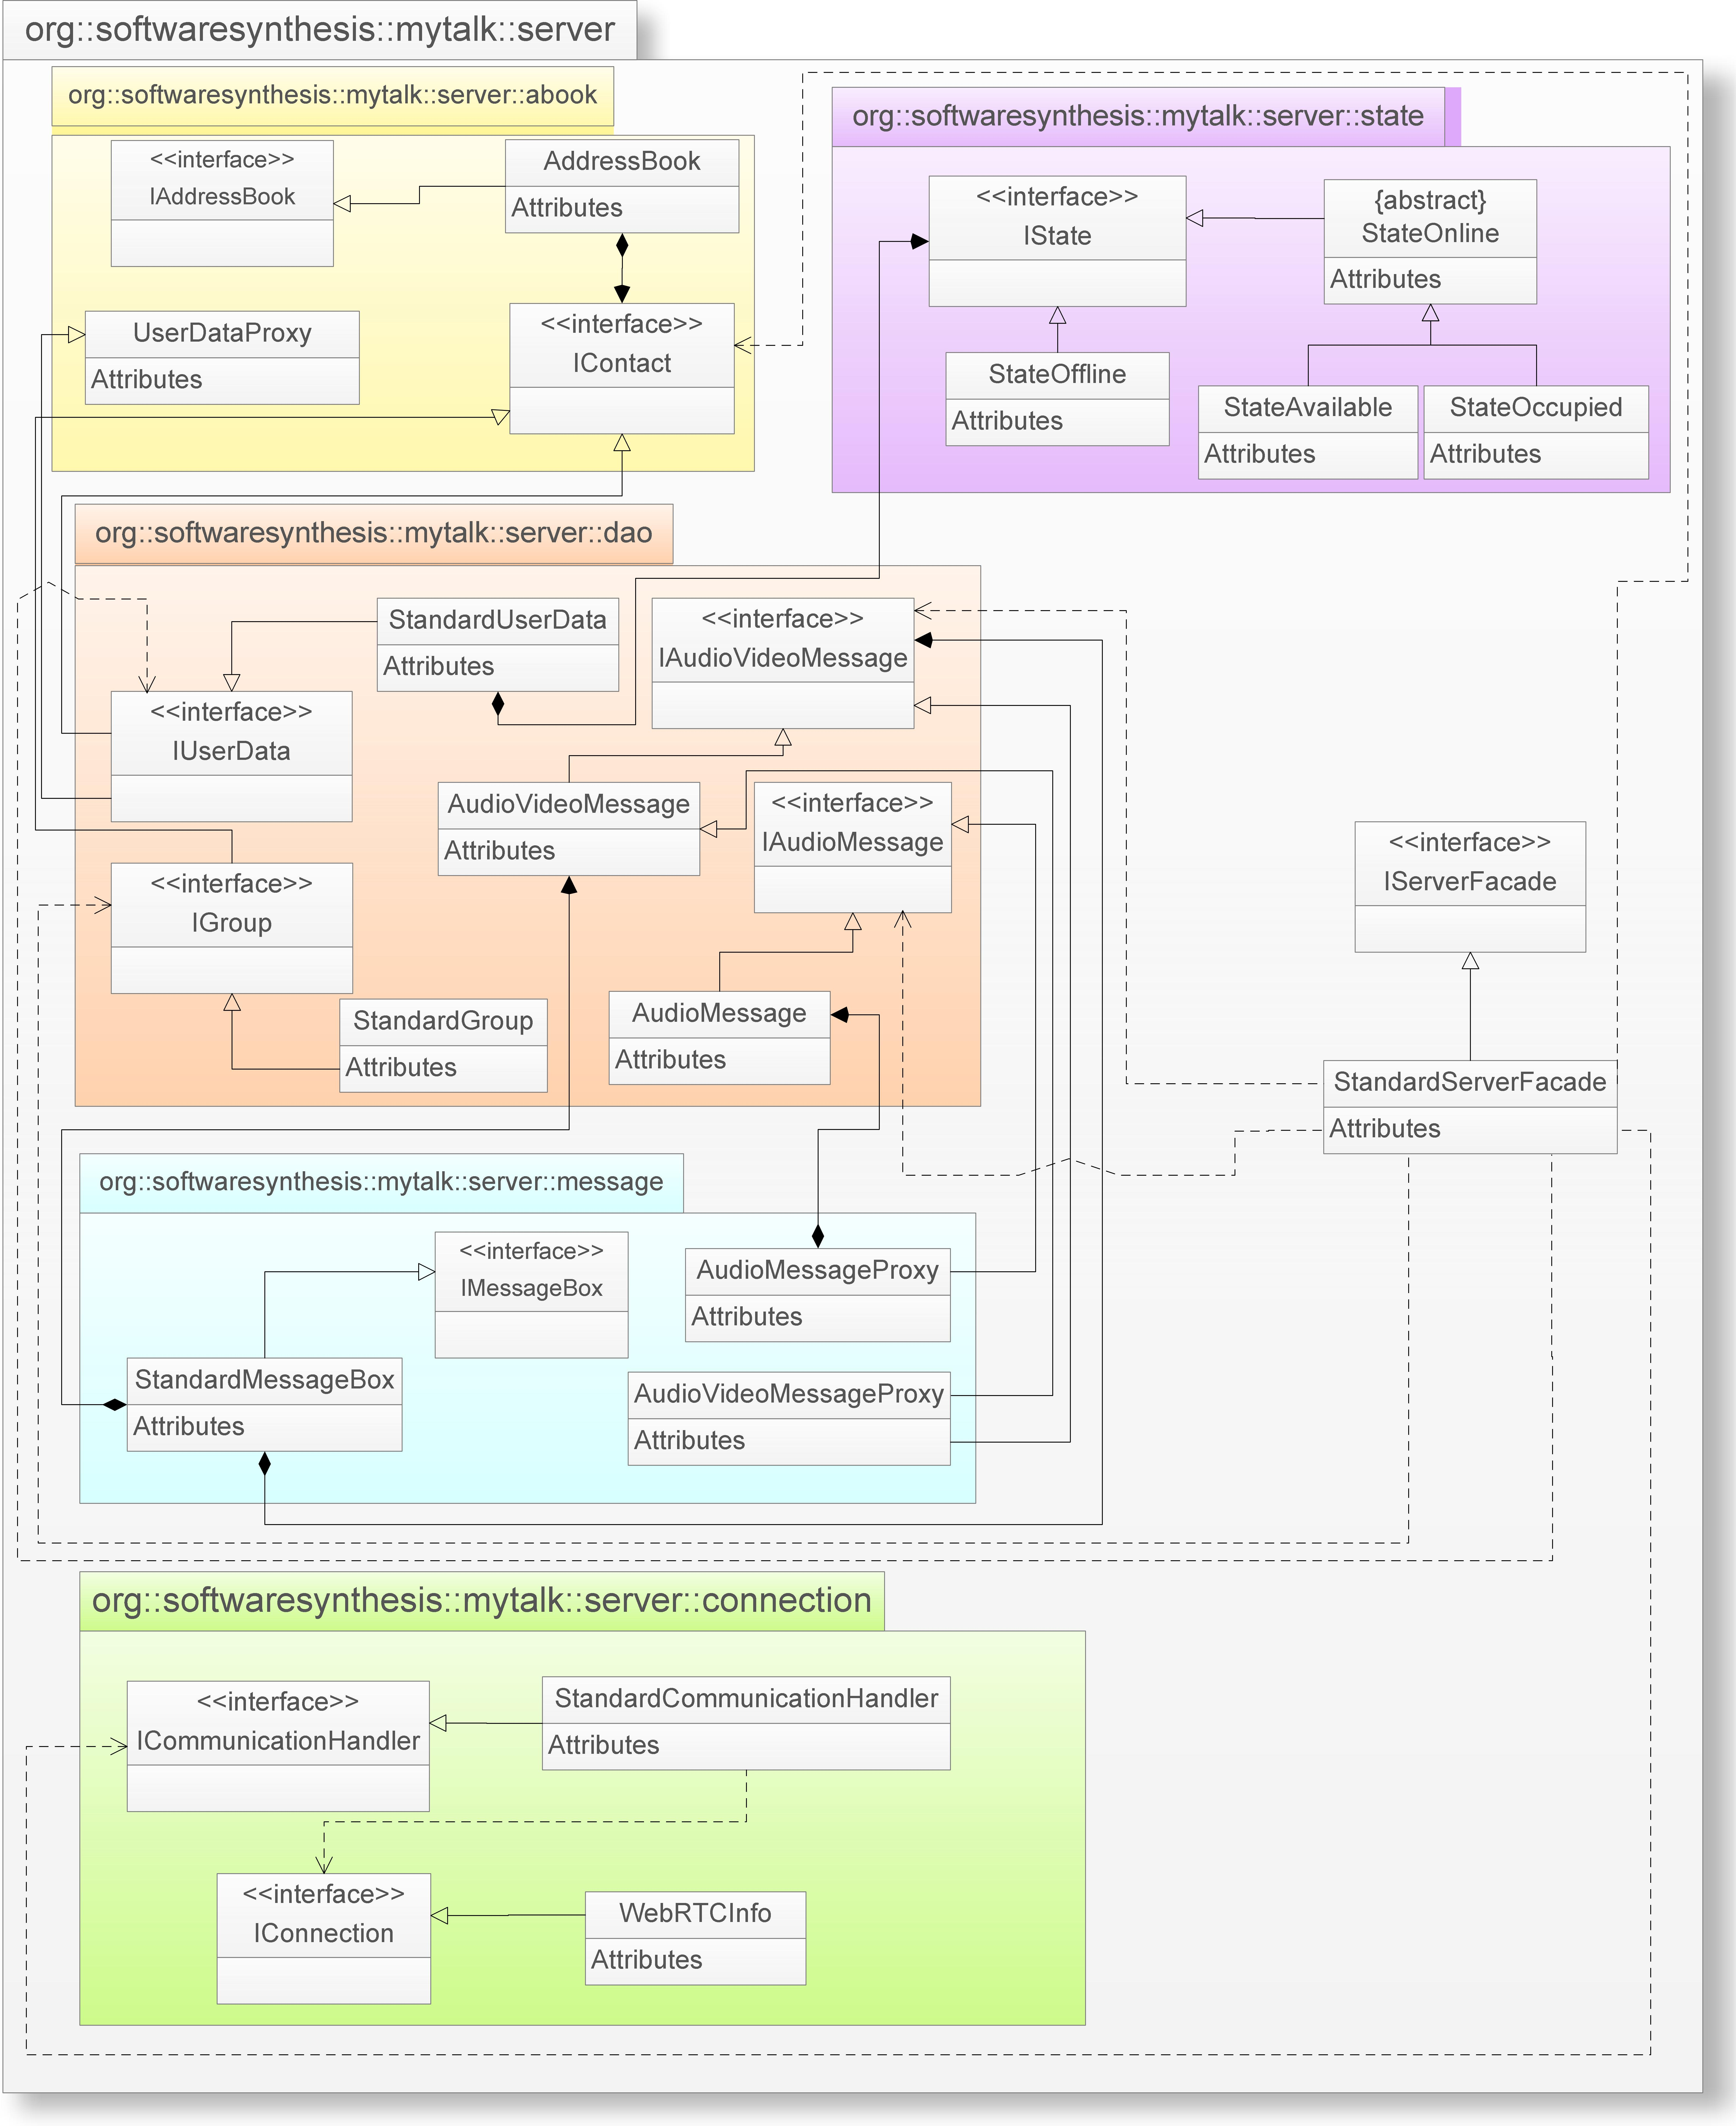
\includegraphics[width=1\textwidth]{server_generale}
  \caption{Diagramma delle classi - Architettura \texttt{mytalk.server}}\label{fig:sottoarchserver}
\end{figure}

Il diagramma in figura \ref{fig:sottoarchserver} rappresenta solo ed esclusivamente le classi definite in sede di progettazione architetturale e non riporta invece tutte le interfacce/classi appartenenti a librerie esterne (ad es. \texttt{javax.servlet.http.HttpServlet}) che sono state estese o implementate nella sotto-architettura server. Tali informazioni, che avrebbero appesantito ulteriormente un diagramma già di grandi dimensioni sono invece riportate nei diagrammi dei singoli componenti.
Inoltre il diagramma non riporta le dipendenze.
\clearpage

\section{Architettura \texttt{mytalk.clientpresenter}}\label{sec:clientpresenter}
La sotto-architettura \texttt{clientpresenter}, nasce con lo scopo di imporre una separazione tra la logica di gestione di un client e l'interfaccia grafica visualizzata all'utente finale.

Dal momento che il \inglese{presenter} ha la responsabilità di ricevere i comandi utente dalla vista e di sovrintendere all'aggiornamento della stessa, è prevista anche la presenza di una serie di oggetti necessari a gestire l'interazione con la vista, corrispondenti al componente \textsf{Gestione GUI}\@.

Dal momento che per l'interazione con l'utente sono previste molteplici viste, è stato predisposto un \inglese{presenter} per ognuna di queste. Ogni vista detiene un riferimento al proprio \inglese{presenter} al quale vengono inviate le richieste su risposta dell'interazione con l'utente, in quanto le operazioni del \inglese{presenter} sono impostate come funzioni di \inglese{callback} nell'interfaccia grafica.

I vari \inglese{presenter} interagiscono con le viste grazie alla conoscenza di una ``interfaccia'' per la loro manipolazione, in quanto tramite \textit{JavaScript} è possibile intervenire sul \underline{DOM}\@. Tali considerazioni sono conformi all'utilizzo del \inglese{design pattern} MVP.\footnote{%
  Per una descrizione più dettagliata del \inglese{pattern} MVP si rimanda alla sezione \ref{sec:MVP}\@.
}

Questo componente ha inoltre il compito di recuperare i dati presenti sul server relativi alla rubrica di un utente, la segreteria telefonica e lo storico delle chiamate che lo interessano. I diversi \inglese{presenter} del componente \textsf{Gestione GUI} hanno dunque anche il compito di interrogare il server al fine di procurarsi le informazioni con cui popolare l'interfaccia grafica utente.

Le informazioni sono rappresentate dalle strutture del componente \textsf{Rappresentazione dati} e permangono internamente al \inglese{presenter} per essere disponibili a successive interrogazioni da parte della GUI senza coinvolgere nuovamente il server.

La logica di comunicazione fra client, e fra client e server, è incapsulata all'interno delle classi facenti parte del componente \textsf{Gestione comunicazione}. Queste ultime sfruttano un canale di comunicazione bidirezionale client-server per interagire con il server in merito alle richieste di comunicazione con altri client, andando a creare appositi canali di comunicazione che si avvalgono della tecnologia WebRTC\@.

In sintesi, la sotto-architettura \texttt{clientpresenter} dispone dei seguenti componenti:
\begin{itemize}[noitemsep,nolistsep]
	\item[-] \textsf{CP01 -- Gestione comunicazione};
	\item[-] \textsf{CP02 -- Rappresentazione dati};
	\item[-] \textsf{CP03 -- Gestione GUI};
\end{itemize}
che saranno descritte con maggiori dettagli nella sezione successiva.

Si ricorda sin da ora che i nomi di tutte le interfacce e tutte le classi riportate nella sezione sono implicitamente parte del package \texttt{org.softwaresynthesis.mytalk.clientpresenter} pertanto tale prefisso sarà omesso nella loro denominazione.

Nella progettazione ad alto livello è stato scelto di non tenere in considerazione il dominio tecnologico dell'applicativo, che non prevede la presenza di classi e interfacce. La progettazione sarà pertanto influenzata unicamente dalle specifiche e dai principi della programmazione orientata agli oggetti.

Tale scelta è motivata dalle seguenti considerazioni:
\begin{itemize}
   \item l'utilizzo dei \inglese{pattern} architetturali necessita a monte di uno stile di progettazione ad oggetti;
   \item così facendo è garantita la possibilità di riuso del risultato progettazione architetturale sotto altri domini tecnologici.
\end{itemize}

La presenza delle interfacce, delle relazioni di implementazione e l'estensione fra classi saranno pertanto mantenute.

\subsection{Componenti evidenziati}

%TODO da rivedere con Tres e Schivo!
\subsubsection{CP01 -- Gestione comunicazione}
\begin{description}
	\item{\scshape\bfseries Descrizione:}\\
È il componente che rappresenta il nucleo logico fondamentale della comunicazione. In esso è presente la classe \texttt{kernel.CommunicationCenter} che ha la responsabilità di tener traccia delle comunicazioni aperte con i client usando la tecnologia WebRTC\@. Per compiere il proprio lavoro, tale classe si avvale delle funzionalità fornite dal webRTC per creare e gestire la comunicazione. Nello specifico vengono usate le classi:

\begin{itemize}
	\item PeerICECandidate;
	\item WebKitRTCPeerConnection;
	\item PeerSessionDescription;
\end{itemize}

	\item{\scshape\bfseries Diagramma delle classi:}
  \begin{figure}[H]
    \centering
    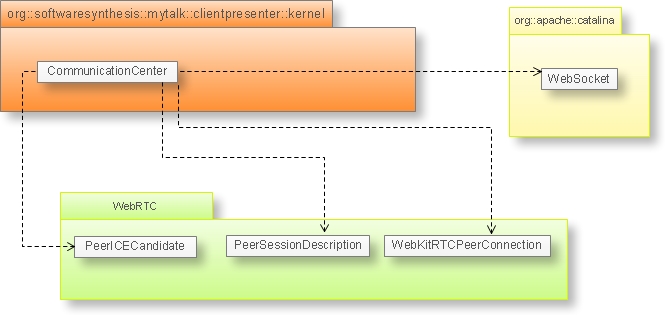
\includegraphics[width=.7\textwidth]{class_gestione_comunicazione_pres}
    \caption{Diagramma delle classi - Gestione comunicazione}\label{fig:gestionecomunicazione}
  \end{figure}

	\item{\scshape\bfseries Classi utilizzate:} 
	\begin{itemize}[noitemsep,nolistsep]
		\item[-] \texttt{kernel.CommunicationCenter}
		\item[-] \texttt{PeerICECandidate}
		\item[-] \texttt{WebKitRTCPeerConnection}
		\item[-] \texttt{PeerSessionDescription}
	\end{itemize}  
\end{description}

\subsubsection{CP02 -- Rappresentazione dati}
\begin{description}
  \item{\scshape\bfseries Descrizione:}\\
Le classi di questo componente hanno il compito di rappresentare sotto forma di apposite strutture dati le informazioni ottenute dall'interrogazione del modello dei dati e ricevute in forma serializzata a seguito delle richieste al server.

La disponibilità di queste informazioni sul client permette una più agevole rappresentazione dell'interfaccia grafica per gli oggetti del componente \textsf{Gestione GUI} ed evita nuove interrogazioni al server qualora i dati in possesso da parte del \inglese{presenter} siano ancora validi.

I dati rappresentati in forma di oggetti sono necessari, in particolare, per la gestione della segreteria, dello storico delle chiamate e della rubrica lato client.

  \item{\scshape\bfseries Diagramma delle classi:}\\
  \begin{figure}[H]
    \centering
    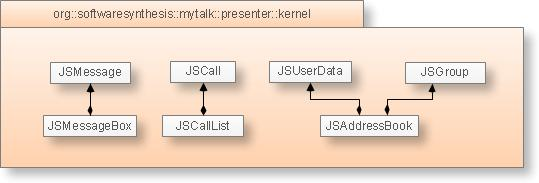
\includegraphics[width=.8\textwidth]{class_rappresentazione_dati}
    \caption{Diagramma delle classi - Rappresentazione dati}\label{fig:rappresentazionedati}
  \end{figure}

	\item{\scshape\bfseries Classi utilizzate:} 
	\begin{itemize}[noitemsep,nolistsep]
		\item[-] \texttt{data.JSCall}
		\item[-] \texttt{data.JSGroup}
		\item[-] \texttt{data.JSMessage}
		\item[-] \texttt{data.JSUserData}
	\end{itemize}  
\end{description}

\subsubsection{CP03 -- Gestione GUI}
\begin{description}
	\item{\scshape\bfseries Descrizione:}\\
Il componente ha il duplice ruolo di intercettare gli eventi che scaturiscono dall'interazione dell'utente con la GUI e di controllare l'aggiornamento della stessa a seguito dei cambiamenti che intervengono sul modello dei dati.

Per quanto riguarda l'autenticazione, è prevista la presenza di un \inglese{presenter} per l'interfaccia di \inglese{login}, corrispondente all'oggetto \texttt{guicontrol.LoginPresenter}. Anche per la registrazione vale la stessa considerazione e tale funzionalità è destinata alla classe \texttt{guicontrol.RegisterPresenter}

Per quanto riguarda invece la pagina principale dell'applicativo, alla quale si accede dopo aver effettuato l'autenticazione, è prevista la presenza di tre tipi principali di \inglese{presenter}:
\begin{itemize}[noitemsep,nolistsep]
  \item[-] \texttt{guicontrol.AddressBookPresenter}, che gestisce il pannello della rubrica presente nell'interfaccia grafica;
  \item[-] \texttt{guicontrol.MainPresenter}, alla radice di una gerarchia di \inglese{presenter} destinati a gestire gli elementi che compaiono nella parte centrale dell'interfaccia grafica, comprende alcune operazioni comuni a questi elementi grafici (ad es. per l'inizializzazione o per la comparsa/scomparsa dell'elemento grafico associato);
  \item[-] \texttt{guicontrol.ToolsPresenter}, che ha il compito di gestire il pannello degli strumenti nell'interfaccia grafica.
\end{itemize}

La struttura delle classi che lo compongono mostra una corrispondenza biunivoca con gli elementi grafici presentati nella sezione~\ref{sec:clientview} con un \inglese{presenter} per ognuno dei pannelli cui si aggiunge un oggetto istanza di \texttt{guicontrol.PresenterMediator}.

Ogni \inglese{presenter} facente parte di questo componente contiene al suo interno le funzioni di \inglese{callback} che vengono richiamate dall'elemento dell'interfaccia grafica corrispondente.

Dal momento che il componente \textsf{Gestione GUI} è anche responsabile anche delle modifiche alle viste, le sottoclassi di \texttt{guicontrol.MainPresenter} contengono anche le operazioni richiamate dall'esterno per l'aggiornamento dinamico della GUI\@.

L'oggetto \texttt{PresenterMediator} invece incapsula la collaborazione fra i vari \inglese{presenter} associati alla grafica e permette di gestire gli eventi generati da un elemento della GUI inviando a uno (o più) \inglese{presenter} i messaggi corrispondenti alle azioni da compiere.

	\item{\scshape\bfseries Diagramma delle classi:}\\
  \begin{figure}[H]
    \centering
    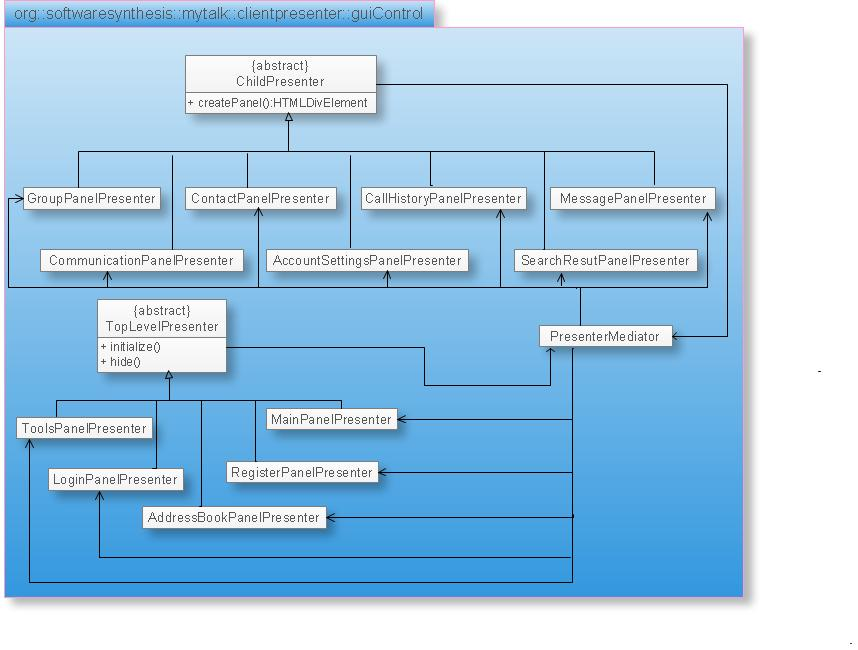
\includegraphics[width=.9\textwidth]{class_gestione_gui}
    \caption{Diagramma delle classi - Gestione GUI}\label{fig:gestionegui}
  \end{figure}

	\item{\scshape\bfseries Classi utilizzate:}\\
	\begin{itemize}[noitemsep,nolistsep]
	  \item[-] \texttt{guicontrol.AccountSettingsPresenter}
	  \item[-] \texttt{guicontrol.AddressBookPresenter}
	  \item[-] \texttt{guicontrol.CallHistoryPresenter}
	  \item[-] \texttt{guicontrol.CommunicationPresenter}
	  \item[-] \texttt{guicontrol.GroupPresenter}	 
	  \item[-] \texttt{guicontrol.SearchResultPresenter}	   
	  \item[-] \texttt{guicontrol.ContactPresenter}
	  \item[-] \texttt{guicontrol.LoginPresenter}
	  \item[-] \texttt{guicontrol.RegisterPresenter}	 
	  \item[-] \texttt{guicontrol.TopLevelPresenter}	  
	  \item[-] \texttt{guicontrol.ChildPrenter}	  
	  \item[-] \texttt{guicontrol.MainPresenter}
		\item[-] \texttt{guicontrol.MessagePresenter}
		\item[-] \texttt{guicontrol.PresenterMediator}
	  \item[-] \texttt{guicontrol.ToolsPresenter}
	\end{itemize}
\end{description}

\subsection{Descrizione delle classi}

\subsubsection{Package \texttt{org.softwaresynthesis.mytalk.clientpresenter.kernel}}

\begin{itemize}[leftmargin=0em]

%TODO da rivedere con Tres e Schivo!
\item \texttt{CommunicationCenter}
\begin{description}
	\item{\scshape\bfseries Descrizione:}\\
È la classe che ha il compito di gestire la comunicazione con il server reagendo agli eventi che si verificano alla ricezione di un messaggio tramite il canale \texttt{server.connection.PushInBound} (nel caso di una comunicazione entrante) oppure inviando tali messaggi al server (nel caso di una comunicazione uscente), al fine di stabilire una comunicazione client-client di tipo WebRTC\@.

Tale classe è inoltre stata implementata come Singleton, al fine di porre un limite superiore pari a uno al numero di istanze che sono presenti in ciascun client.

	\item{\scshape\bfseries Componenti che ne fanno uso:}
	\begin{itemize}[noitemsep,nolistsep]
	  \item[-] \textsf{CP01 -- Gestione comunicazione}
	\end{itemize}
\end{description}

\end{itemize}

\subsubsection{Package \texttt{org.softwaresynthesis.mytalk.clientpresenter.data}}

\begin{itemize}[leftmargin=0em]

\item \texttt{JSCall}
\begin{description}
  \item{\scshape\bfseries Descrizione:}\\
Tale classe modella una chiamata appartenente allo storico dell'utente corrente (dove risiede il \inglese{presenter}), e permette di accedere alle informazioni caratteristiche quali il mittente, l'insieme dei destinatari, la durata e la data di inizio della chiamata, sia essa di natura audio oppure audio/video.

Qualora lo storico delle chiamate non fosse disponibile sul client in cui è ospitato il \inglese{presenter}, gli oggetti di tipo \texttt{JSCall} sono creati a seguito di una richiesta da parte di \texttt{guicontrol.CallHistoryPresenter} al fine di ottenere i dati che devono essere visualizzati nell'interfaccia grafica.

  \item{\scshape\bfseries Componenti che ne fanno uso:}
	\begin{itemize}[noitemsep,nolistsep]
	  \item[-] \textsf{CP02 -- Rappresentazione dati}
	  \item[-] \textsf{CP03 -- Gestione GUI}
	\end{itemize}
\end{description}

\item \texttt{JSMessage}
\begin{description}
  \item{\scshape\bfseries Descrizione:}\\
Classe che rappresenta un messaggio presente nella segreteria dell'utente corrente.

I diversi \inglese{presenter} del componente \textsf{Gestione GUI} possono accedere al mittente del messaggio, allo stato del messaggio (ascoltato o non ascoltato), alla natura del messaggio (audio o audio/video), alla durata e, in ultima istanza, al contenuto del messaggio.

I messaggi della segreteria telefonica di un determinato utente vengono scaricati dal \inglese{presenter} \texttt{guicontrol.MessagePresenter} qualora non fossero presenti sul client che ospita il \inglese{presenter} e sono in seguito utilizzati per popolare l'interfaccia grafica.

  \item{\scshape\bfseries Componenti che ne fanno uso:}
	\begin{itemize}[noitemsep,nolistsep]
	  \item[-] \textsf{CP02 -- Rappresentazione dati}
	  \item[-] \textsf{CP03 -- Gestione GUI}
	\end{itemize}
\end{description}

\item \texttt{JSUserData}
\begin{description}
  \item{\scshape\bfseries Descrizione:}\\
Tale classe ha il compito di rappresentare i contatti della rubrica lato \inglese{presenter}, generata serializzando esclusivamente la parte che si vuole trasmettere ai client delle istanze del \inglese{transfer object} descritto sopra (\texttt{org.softwaresynthesis.mytalk.server.abook.UserData}).

In particolare, di un utente-contatto è possibile ottenere lo \inglese{username}, i dati anagrafici (nome e cognome) nonché l'immagine associata al profilo personale, laddove queste ultime tre informazioni sono da considerarsi facoltative e potrebbero non essere disponibili per un determinato utente.

Gli oggetti \texttt{JSUserData} vengono creati a seguito di una richiesta proveniente dal \inglese{presenter} \texttt{guicontrol.AddressBookPresenter} e sono successivamente impiegati  al fine di popolare l'interfaccia grafica con i dati corrispondenti alla rubrica utente.

  \item{\scshape\bfseries Componenti che ne fanno uso:}
	\begin{itemize}[noitemsep,nolistsep]
	  \item[-] \textsf{CP02 -- Rappresentazione dati}
	  \item[-] \textsf{CP03 -- Gestione GUI}
	\end{itemize}
\end{description}

\item \texttt{JSGroup}
\begin{description}
  \item{\scshape\bfseries Descrizione:}\\
Classe avente il compito di rappresentare i gruppi della rubrica lato \inglese{presenter}, generata serializzando esclusivamente la parte che si vuole trasmettere ai client delle istanze del \inglese{transfer object} descritto sopra (\texttt{org.softwaresynthesis.mytalk.server.abook.Group}).

In particolare di un gruppo è possibile ottenere il nome e l'elenco dei contatti appartenenti al gruppo.

Gli oggetti \texttt{JSGroup} vengono creati a seguito di una richiesta proveniente dal \inglese{presenter} \texttt{guicontrol.GroupPresenter} e sono successivamente impiegati  al fine di popolare l'interfaccia grafica con la lista dei gruppi utente.

  \item{\scshape\bfseries Componenti che ne fanno uso:}
	\begin{itemize}[noitemsep,nolistsep]
	  \item[-] \textsf{CP02 -- Rappresentazione dati}
	  \item[-] \textsf{CP03 -- Gestione GUI}
	\end{itemize}
\end{description}

\end{itemize}

\subsubsection{Package \texttt{org.softwaresynthesis.mytalk.clientpresenter.guicontrol}}
\begin{itemize}[noitemsep,nolistsep]

\item \texttt{guicontrol.AccountSettingsPresenter}
\begin{description}
	\item{\scshape\bfseries Descrizione:}\\
Si tratta del \inglese{presenter} richiamato dall'elemento grafico corrispondente al pannello \texttt{org.softwaresynthesis.mytalk.clientview.AccountSettingsPresenter} per la gestione dei dati relativi all'utente associato al client.

Per questo motivo, l'oggetto \texttt{AccountSettingsPresenter} ha il compito di mettere a disposizione per la vista le funzioni di \inglese{callback} che comportano la modifica di questi stessi dati. 

	\item{\scshape\bfseries Componenti che ne fanno uso:}
	\begin{itemize}[noitemsep,nolistsep]
	  \item[-] \textsf{CP03 -- Gestione GUI}
	  \item[-] \textsf{CV01 -- GUI}
	\end{itemize}
\end{description}

\item \texttt{guicontrol.AddressBookPresenter}
\begin{description}
	\item{\scshape\bfseries Descrizione:}\\
Tale \inglese{presenter} viene richiamato dall'elemento grafico corrispondente al pannello della rubrica (\texttt{org.softwaresynthesis.mytalk.clientview.AddressBookPresenter}) e contiene la risposta a eventi quali la selezione di un contatto dalla rubrica da parte dell'utente. Contiene inoltre un'operazione di \inglese{refresh} che visualizza una lista di contatti ricevuta in input in forma grafica sulla UI\@.

Il \inglese{presenter} in questione rende inoltre possibile avviare una ricerca fra gli utenti registrati nel sistema nonché rilevare che l'operazione di ricerca è conclusa (e conseguentemente visualizzare nuovamente la rubrica). 


I dati corrispondenti alla rubrica, ovvero le corrispondenti istanze di classi definite in \textsf{Rappresentazione dati}, se non sono presenti sul client devono essere recuperati dal server ed è responsabilità di questa classe contattare la \textsf{Gestione controller} al fine di ottenere le informazioni necessarie.

Infine in modo simile sono comunicati al server gli esiti delle operazioni di amministrazione sulla rubrica che hanno un effetto sulle informazioni di modello.

	\item{\scshape\bfseries Componenti che ne fanno uso:}
	\begin{itemize}[noitemsep,nolistsep]
	  \item[-] \textsf{CP03 -- Gestione GUI}
	  \item[-] \textsf{CV01 -- GUI}
	\end{itemize}
\end{description}

\item \texttt{guicontrol.CallHistoryPresenter}
\begin{description}
	\item{\scshape\bfseries Descrizione:}\\
Questo \inglese{presenter} gestisce l'elemento corrispondente al pannello dello storico delle chiamate presente nell'interfaccia grafica, permettendo la visualizzazione di un \textit{array} di chiamate corrispondenti alle comunicazioni di un determinato utente.

Poiché il componente grafico supervisionato è totalmente passivo, non sono presenti operazioni di \inglese{callback} da associare alle componenti grafiche vere e proprie.

Qualora i dati corrispondenti allo storico delle chiamate non fossero disponibili sul client che ospita questo \inglese{presenter} è responsabilità di quest'ultimo interrogare il server (attraverso il componente \textsf{Gestione controller}) al fine di ottenere le informazioni necessarie.

	\item{\scshape\bfseries Componenti che ne fanno uso:}
	\begin{itemize}[noitemsep,nolistsep]
	  \item[-] \textsf{CP03 -- Gestione GUI}
	  \item[-] \textsf{CV01 -- GUI}
	\end{itemize}
\end{description}

\item \texttt{guicontrol.CommunicationPresenter}
\begin{description}
	\item{\scshape\bfseries Descrizione:}\\
Tale \inglese{presenter} si occupa della gestione del componente grafico corrispondente al pannello di comunicazione fra utenti. In particolare, comprende le operazioni necessarie all'aggiornamento della grafica corrispondente alle chat testuali e alle condivisioni, nonché alla visualizzazione dello \inglese{stream} video nel corso di una comunicazione audio/video o dell'immagine associata al profilo utente nel caso di una sola comunicazione audio.

Le principali funzioni di \inglese{callback} utilizzate dall'interfaccia grafica presenti in questa classe corrispondono alla possibilità di interrompere una chiamata in corso, avviare/interrompere una condivisone di risorse, avviare/interrompere una registrazione, visualizzare/nascondere le aree di chat (che sono indipendenti dalla comunicazione corrente).

	\item{\scshape\bfseries Componenti che ne fanno uso:}
	\begin{itemize}[noitemsep,nolistsep]
	  \item[-] \textsf{CP03 -- Gestione GUI}
	  \item[-] \textsf{CV01 -- GUI}
	\end{itemize}
\end{description}

\item \texttt{guicontrol.ContactPresenter}
\begin{description}
	\item{\scshape\bfseries Descrizione:}\\
Tale \inglese{presenter} ha la responsabilità di controllare l'aggiornamento della sezione dell'interfaccia grafica incaricata di visualizzare il profilo di un utente in risposta alla selezione dalla rubrica o dall'esito di una ricerca.

Poiché inoltre, a partire da tale componente grafico è possibile avviare una comunicazione, tale classe comprende al proprio interno anche le funzioni che devono essere richiamate in risposta all'azione da parte dell'utente di dare avvio a una comunicazione.

Poiché da \texttt{org.softwaresynthesis.mytalk.clientview.ContactPresenter} è possibile anche svolgere alcune attività di amministrazione della rubrica utente, in questo \inglese{presenter} sono presenti anche le funzioni di \inglese{callback} necessarie per l'aggiunta e la rimozione di un contatto particolare ad un gruppo, bloccare o sbloccare tale contatto, nonché per l'aggiunta dello stesso alla rubrica se il suo profilo è stato aperto a seguito di una ricerca fra gli utenti registrati nel sistema.

Dal momento che, infine, tali operazioni di amministrazione hanno un effetto sulle entità del modello dei dati che risiedono sul server, tale classe ha la responsabilità di notificare gli aggiornamenti sul server al fine di mantenere la consistenza delle informazioni.

	\item{\scshape\bfseries Componenti che ne fanno uso:}
	\begin{itemize}[noitemsep,nolistsep]
	  \item[-] \textsf{CP03 -- Gestione GUI}
	  \item[-] \textsf{CV01 -- GUI}
	\end{itemize}
\end{description}

\item \texttt{guicontrol.GroupPresenter}
\begin{description}
	\item{\scshape\bfseries Descrizione:}\\
Tale \inglese{presenter} ha la responsabilità di controllare l'aggiornamento della sezione dell'interfaccia grafica incaricata all'amministrazione dei gruppi creati dall'utente in risposta alla modifica (intesa come aggiunta o rimozione) di tali gruppi tramite le funzioni di \inglese{callback} associate.
%TODO DA FUFFARE, NON SONO COSì ABILE PURTROPPO -.-'

	\item{\scshape\bfseries Componenti che ne fanno uso:}
	\begin{itemize}[noitemsep,nolistsep]
	  \item[-] \textsf{CP03 -- Gestione GUI} %TODO AGGIORNARE COMPONENTI CHE LA USANO
	  \item[-] \textsf{CV01 -- GUI}
	\end{itemize}
\end{description}


%CLASSE MORTA (SELETTORE LINGUA DELLA GUI)
%\item \texttt{guicontrol.LanguagePresenter}
%\begin{description}
%	\item{\scshape\bfseries Descrizione:}\\
%Il \inglese{presenter} in questione ha il compito di popolare il contenuto dell'elemento grafico corrispondente al pannello di configurazione della UI e, in particolare, della lingua in cui questa viene visualizzata.

%Contiene un'unica operazione di \inglese{callback} per la grafica, che riceve la selezione dell'utente %e propaga le modifiche a tutti i \inglese{presenter} associati alle componenti grafiche. Non %ammette invece alcuna operazione di aggiornamento della GUI in quanto gli elementi da %visualizzare sono noti al momento dell'inizializzazione e non subiscono modifiche ulteriori a %tempo di esecuzione.

%	\item{\scshape\bfseries Componenti che ne fanno uso:}
%	\begin{itemize}[noitemsep,nolistsep]
%	  \item[-] \textsf{CP03 -- Gestione GUI}
%	  \item[-] \textsf{CV01 -- GUI}
%	\end{itemize}
%\end{description}

\item \texttt{guicontrol.LoginPresenter}
\begin{description}
  \item{\scshape\bfseries Descrizione:}\\
Tale \inglese{presenter} ha il compito di ricevere dall'interfaccia grafica i dati di autenticazione, associando un suo metodo all'evento \texttt{onSubmit} del \inglese{form} di \inglese{login}, e in seguito inoltrarli alla sotto-architettura server tramite una \inglese{servlet} del componente \textsf{Gestione controller}.

L'oggetto \texttt{LoginPresenter} permette semplicemente di comunicare al server i dati di \inglese{login} inseriti dall'utente.
  
  \item{\scshape\bfseries Componenti che ne fanno uso:}
  \begin{itemize}[noitemsep,nolistsep]
    \item[-] \textsf{CP03 -- Gestione GUI}
	  \item[-] \textsf{CV02 -- Login}
  \end{itemize}
\end{description}

\item \texttt{guicontrol.MainPresenter}
\begin{description}
	\item{\scshape\bfseries Descrizione:}\\
Classe base per i \inglese{presenter} associati ai diversi componenti dell'interfaccia grafica che contiene i metodi necessari all'inizializzazione di questi ultimi nonché i controlli che ne attivano la comparsa o scomparsa in risposta alle preferenze di visualizzazione dell'utente.

	\item{\scshape\bfseries Componenti che ne fanno uso:}
	\begin{itemize}[noitemsep,nolistsep]
	  \item[-] \textsf{CP03 -- Gestione GUI}
	  \item[-] \textsf{CV01 -- GUI}
	\end{itemize}
\end{description}

\item \texttt{guicontrol.MessagePresenter}
\begin{description}
	\item{\scshape\bfseries Descrizione:}\\
Tale \inglese{presenter} contiene le operazioni necessarie a visualizzare l'elenco dei messaggi presenti nella segreteria telefonica di un determinato utente.

Poiché a partire dalla vista associata è possibile avviare/arrestare la riproduzione di un messaggio, questo oggetto deve contenere opportune funzioni di \inglese{callback} per rispondere alle richieste dell'utente in tal senso. La cancellazione di un messaggio, corrispondente al requisito RUFF15.4.0, è anch'essa possibile attraverso un'operazione di questo \inglese{presenter}, così come il cambiamento di stato del messaggio una volta che viene ascoltato.

È prevista inoltre la possibilità di aggiornamento del componente grafico, in quanto la ricezione di nuovi messaggi può avvenire anche se l'utente è in linea (ad esempio se questi è impegnato in un'altra conversazione).

Qualora i dati corrispondenti alla segreteria telefonica di un utente non fossero disponibili sul client, è responsabilità di questa classe interrogare il server al fine di ottenere le informazioni necessarie nonché istanziare le opportune classi di \textsf{Rappresentazione dati}.

Infine, per le operazioni che hanno effetto sulla rappresentazione del modello dei dati sul server, quali la cancellazione di un messaggio o il cambiamento di stato di un messaggio, devono essere notificati al server attraverso il componente \textsf{Gestione controller}.

	\item{\scshape\bfseries Componenti che ne fanno uso:}
	\begin{itemize}[noitemsep,nolistsep]
	  \item[-] \textsf{CP03 -- Gestione GUI}
	  \item[-] \textsf{CV01 -- GUI}
	\end{itemize}
\end{description}

\item \texttt{guicontrol.PresenterMediator}
\begin{description}
	\item{\scshape\bfseries Descrizione:}\\
L'istanza di tale classe ha il compito di gestire le collaborazioni fra i diversi \inglese{presenter} associati alle viste dell'interfaccia grafica e smistare i messaggi che questi si devono scambiare.

A tale scopo, è necessario che tutti i \inglese{presenter} si registrino su di essa in modo da poter ricevere le successive richieste tramite chiamata di metodo. Inoltre, questi ultimi sono in grado di notificare gli eventi di interesse al \texttt{PresenterMediator} che resta costantemente in ascolto su di essi.

	\item{\scshape\bfseries Componenti che ne fanno uso:}
	\begin{itemize}[noitemsep,nolistsep]
	  \item[-] \textsf{CP03 -- Gestione GUI}
	  \item[-] \textsf{CP04 -- Gestione remota}
	\end{itemize}
\end{description}


\item \texttt{guicontrol.RegisterPresenter}
\begin{description}
	\item{\scshape\bfseries Descrizione:}\\
Tale \inglese{presenter} ha il compito di ricevere dall'interfaccia grafica i dati con cui desidera registrarsi un utente, associando un suo metodo all'evento \texttt{onSubmit} del \inglese{form} di registrazione, e in seguito inoltrarli alla sotto-architettura server tramite una \inglese{servlet} del componente \textsf{Gestione controller}.

	\item{\scshape\bfseries Componenti che ne fanno uso:}
	\begin{itemize}[noitemsep,nolistsep]
	  \item[-] \textsf{CP03 -- Gestione GUI}
	  \item[-] \textsf{CV01 -- Login}
	\end{itemize}
\end{description}

\item \texttt{guicontrol.SearchResultPresenter}
\begin{description}
	\item{\scshape\bfseries Descrizione:}\\
Tale \inglese{presenter} ha la responsabilità di controllare l'aggiornamento della sezione dell'interfaccia grafica incaricata della ricerca di un contatto tra quelli iscritti al sistema dopo la richiesta specifica dell'utente.

Per questo motivo, l'oggetto \texttt{SearchResultPresenter} ha il compito di mettere a disposizione per la vista le funzioni di \inglese{callback} che comportano la modifica della stringa di ricerca di uno specifico contatto nella lista.

%TODO CONTROLLARE E INTEGRARE

	\item{\scshape\bfseries Componenti che ne fanno uso:}
	\begin{itemize}[noitemsep,nolistsep]
	  \item[-] \textsf{CP03 -- Gestione GUI} 
	  \item[-] \textsf{CV01 -- GUI}
	\end{itemize}
\end{description}


\item \texttt{guicontrol.ToolsPresenter}
\begin{description}
	\item{\scshape\bfseries Descrizione:}\\
Tramite tale \inglese{presenter} è possibile inizializzare la barra laterale degli strumenti rappresentata da \texttt{org.softwaresynthesis.mytalk.clientview.ToolsPresenter}. Gli aggiornamenti cui tale porzione della vista è soggetta consistono nella visualizzazione/scomparsa di uno o più strumenti su richiesta dell'utente e per ognuno di questi è prevista la presenza di un'operazione.

D'altra parte, gli eventi scatenati dall'interazione dell'utente con il pannello degli strumenti che comportano la modifica dell'elemento mostrato nella regione centrale al posto del pannello principale, sono raccolti da questo \inglese{presenter} e inoltrati al \texttt{PresenterMediator} per la gestione.

In tal modo è possibile far comparire o scomparire il pannello di gestione dei dati personali corrispondenti al proprio account, della segreteria, la gestione dei gruppi e lo storico delle chiamate.

Poiché inoltre da \texttt{org.softwaresynthesis.mytalk.clienview.ToolsPresenter} è possibile impostare il proprio stato, il \inglese{presenter} ad esso associato contiene le funzioni che notificano l'avvenuto cambiamento di stato al componente \textsf{Gestione controller}.

	\item{\scshape\bfseries Componenti che ne fanno uso:}
	\begin{itemize}[noitemsep,nolistsep]
	  \item[-] \textsf{CP03 -- Gestione GUI}
	  \item[-] \textsf{CV01 -- GUI}
	\end{itemize}
\end{description}

\end{itemize}

\begin{figure}[H]
  \centering
  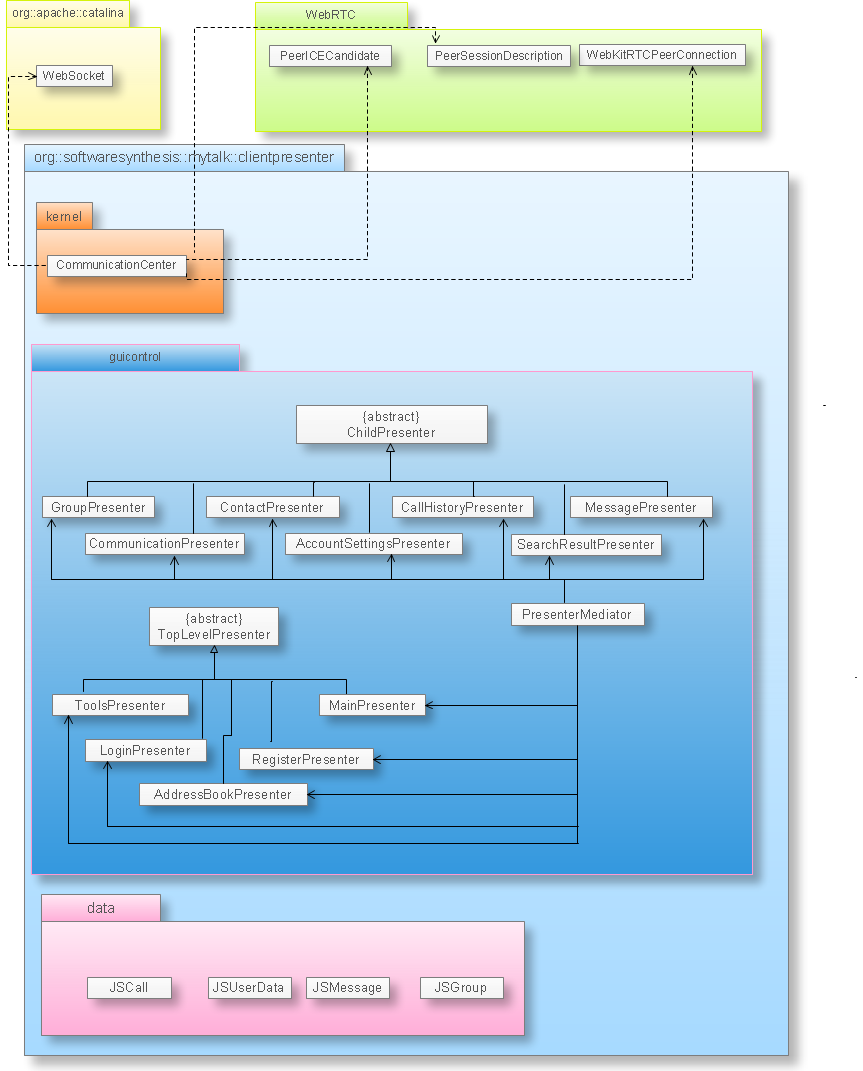
\includegraphics[width=.8\textwidth]{presenter_generale}
  \caption{Diagramma delle classi - Architettura \texttt{mytalk.clientpresenter}}\label{fig:sottoarchpresenter}
  \end{figure}
\clearpage

\section{Architettura \texttt{mytalk.clientview}}\label{sec:clientview}
Come accennato in precedenza, nella sezione \ref{sec:introdesign} e \ref{sec:clientpresenter}, \texttt{clientview} ha il compito di definire la struttura di visualizzazione dei dati costituendo la GUI del sistema lato client.

Le motivazioni che hanno portato a separare tale sotto-architettura dalla parte logica sono da ricercare nei vantaggi di riutilizzo del codice e semplificazione della manutenzione:
\begin{itemize}
 	\item \textbf{future espansioni}: innanzitutto tale scelta permetterà ai progettisti di sviluppare (in futuro) molteplici tipologie di ``viste'', implementabili liberamente svincolando i programmatori dal conoscere al dettaglio la logica sottostante per la gestione delle comunicazioni.
 	\item \textbf{semplificare la manutenzione}: così come scrivere da zero una nuova vista, anche modificare quelle già presenti risulta essere più facile, per gli stessi motivi descritti al punto precedente.
\end{itemize}

La sotto-architettura \texttt{clientview} rappresenta quindi una vista di \inglese{default} fornita dal team, con lo scopo di rappresentare in modo chiaro ed organizzato le possibilità di interazione da parte dell'utente finale con l'applicativo \caName.

Nell'utilizzare tale vista l'utente non avrà alcuna percezione di come sia stata progettata l'architettura totale del sistema, svincolandolo cosi dal dover conoscere le procedure necessarie all'esecuzione di una determinata operazione.

In figura \ref{fig: gui_alto} si riporta un abbozzo dell'interfaccia grafica utente realizzata mediante le classi di questa sotto-architettura. In conformità con quanto stabilito dai requisiti (RSDO10.0.0) l'interfaccia si sviluppa in un'unica pagina.

\begin{figure}[h]
  \centering
  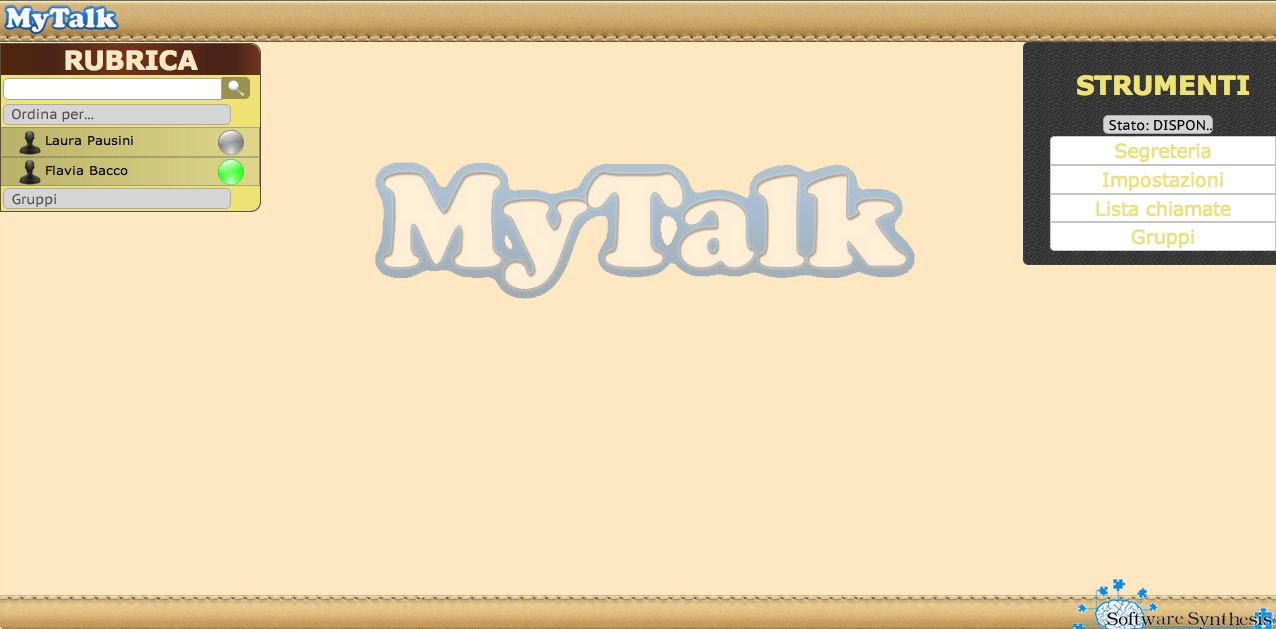
\includegraphics[width=.9\textwidth]{manual_main}
  \caption{Rappresentazione ad alto livello della GUI}\label{fig: gui_alto}
\end{figure}

Per quanto riguarda la componentistica, la sotto-architettura \texttt{clientview} è costituita dai seguenti componenti:
\begin{itemize}[noitemsep,nolistsep]
  \item[-] \textsf{CV01 -- GUI};
  \item[-] \textsf{CV02 -- Login};
\end{itemize}
per le specifiche del quale si rimanda, rispettivamente, alle sezioni \ref{sec:cv01} e \ref{sec:cv02}.

I nomi di tutte le classi riportate nella presente sezione sono inoltre implicitamente parte del package \texttt{org.softwaresynthesis.mytalk.clientview}, pertanto tale prefisso sarà omesso nella loro denominazione.

Analogamente a quanto osservato per la sotto-architettura \texttt{clientpresenter}, la rappresentazione tramite classi e oggetti è utilizzata a livello prettamente logico indipendentemente dal dominio applicativo concreto di implementazione.

In riferimento alla bozza di interfaccia utente presentata in figura \vref{fig: gui_alto}, la parte denominata \texttt{AddressBookView} conterrà la lista degli utenti nella rubrica, mentre \texttt{ToolsPresenteriew} conterrà i componenti grafici che rappresentano tutte le funzionalità offerte dal sistema. 

Il contenuto del \texttt{MainView}, invece, è destinato in relazione alla funzionalità scelta dall'utente in quel momento. Ad esempio, qualora l'utente selezioni un contatto presente nella rubrica, verrà visualizzato il profilo corrispondente al contatto scelto in \texttt{ContactView}, mentre nel caso in cui si attiva una forma di comunicazione, sarà visibile la parte grafica di un'istanza di \texttt{CommunicationView}.

\subsection{Componenti evidenziati}

\subsubsection{CV01 -- GUI}\label{sec:cv01}
\begin{description}
	\item{\scshape\bfseries Descrizione:}\\
Questo componente si occupa della presentazione dell'interfaccia grafica presentata all'utente finale. Le classi in esso contenute servono pertanto per la visualizzazione dei punti di accesso alle funzionalità offerte dal sistema all'utente.

Si noti che tale componente demanda tutta la logica di applicazione al \inglese{presenter} ed è quindi relativo solo ed esclusivamente alla grafica. Tutti i pannelli, che corrispondono ad altrettante viste, hanno pertanto un canale di comunicazione aperto con il \inglese{presenter} loro associato, e gli eventi generati dall'utente devono essere gestiti collegando l'evento alle opportune funzioni di \inglese{callback} offerte dai \inglese{presenter}.

	\item{\scshape\bfseries Diagramma delle classi:}
  \begin{figure}[H]
    \centering
    
   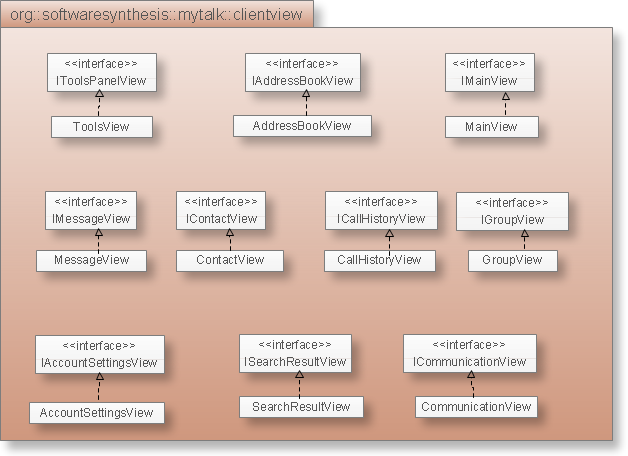
\includegraphics[width=.8\textwidth]{class_gui_panel}
    \caption{Diagramma delle classi - GUI}\label{fig:gui}
  \end{figure}

	\item{\scshape\bfseries Classi utilizzate:} 
	\begin{itemize}[noitemsep,nolistsep]
		\item[-] \texttt{IMainView}
		\item[-] \texttt{IToolsView}
		\item[-] \texttt{IAddressBookView}
		\item[-] \texttt{IContactView}
		\item[-] \texttt{IMessageView}
		\item[-] \texttt{IGroupView}
		\item[-] \texttt{ISearchResultView}
		\item[-] \texttt{IAccountSettingsView}
		\item[-] \texttt{ICallHistoryView}
		\item[-] \texttt{ICommunicationView}
		\item[-] \texttt{MainView}
		\item[-] \texttt{ToolsView}
		\item[-] \texttt{AddressBookView}
		\item[-] \texttt{ContactView}
		\item[-] \texttt{MessageView}
		\item[-] \texttt{GroupView}
		\item[-] \texttt{SearchResultView}
		\item[-] \texttt{AccountSettingsView}
		\item[-] \texttt{CallHistoryView}
		\item[-] \texttt{CommunicationView}
	\end{itemize}  
\end{description}

\subsubsection{CV02 -- Login}\label{sec:cv02}
\begin{description}
  \item{\scshape\bfseries Descrizione:}\\
Il componente \textsf{Login} ha la responsabilità di ricevere in ingresso le credenziali di autenticazione immesse dall'utente del sistema e di trasmetterle al \inglese{presenter} ad esso associato \texttt{org.softwaresynthesis.mytalk.clientpresenter.guicontrol.LoginPresenter}.

	\item{\scshape\bfseries Diagramma delle classi:}
  \begin{figure}[H]
    \centering
    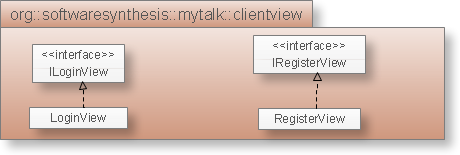
\includegraphics[width=.8\textwidth]{class_gui_login}
    \caption{Diagramma delle classi - Login}\label{fig:login}
  \end{figure}

  \item{\scshape\bfseries Classi utilizzate}
  \begin{itemize}[noitemsep,nolistsep]
  	\item \texttt{ILoginView}
    \item \texttt{IRegisterView}
    \item \texttt{LoginView}
    \item \texttt{RegisterView}
  \end{itemize}

\end{description}

\subsection{Descrizione delle classi}

\subsubsection{Package \texttt{org.softwaresynthesis.clientview}}

\begin{itemize}[leftmargin=0em]

\item \texttt{IAddressBookView}
\begin{description}
  \item{\scshape\bfseries Descrizione}\\
Pannello che permette la visualizzazione della rubrica dell'utente connesso al sistema e di accedere ad alcune delle funzionalità di amministrazione della rubrica stessa (ad esempio l'aggiunta o la rimozione di gruppi).

In questo pannello sono anche presenti le funzionalità di ricerca fra gli utenti presenti nella rubrica, con la visualizzazione dei risultati della ricerca sostituita alla lista dei contatti presenti in rubrica.

  \item{\scshape\bfseries Componenti che ne fanno uso:}
  \begin{itemize}[noitemsep,nolistsep]
    \item[-] \textsf{CV01 -- GUI}
    \item[-] \textsf{CP03 -- Gestione GUI}
  \end{itemize}
\end{description}

\item \texttt{AddressBookView}
\begin{description}
  \item{\scshape\bfseries Descrizione}\\
Implementazione di \texttt{IAddressBookView}.

  \item{\scshape\bfseries Componenti che ne fanno uso:}
  \begin{itemize}[noitemsep,nolistsep]
    \item[-] \textsf{CV01 -- GUI}
    \item[-] \textsf{CP03 -- Gestione GUI}
  \end{itemize}
\end{description}

\item \texttt{IMainView}
\begin{description}
  \item{\scshape\bfseries Descrizione}\\
Classe padre della gerarchia di oggetti grafici che possono comparire nella sezione principale dell'interfaccia utente. Ogni sua specializzazione definisce un nuovo tipo di pannello che costituisce l'elemento in primo piano dell'applicazione.

  \item{\scshape\bfseries Componenti che ne fanno uso:}
  \begin{itemize}[noitemsep,nolistsep]
    \item[-] \textsf{CV01 -- GUI}
    \item[-] \textsf{CP03 -- Gestione GUI}
  \end{itemize}
\end{description}

\item \texttt{MainView}
\begin{description}
  \item{\scshape\bfseries Descrizione}\\
Implementazione di \texttt{IMainView}

  \item{\scshape\bfseries Componenti che ne fanno uso:}
  \begin{itemize}[noitemsep,nolistsep]
    \item[-] \textsf{CV01 -- GUI}
    \item[-] \textsf{CP03 -- Gestione GUI}
  \end{itemize}
\end{description}

\item \texttt{IToolsView}
\begin{description}
  \item{\scshape\bfseries Descrizione}\\
Pannello che rappresenta il pannello degli strumenti della \inglese{home screen} dell'applicativo  mediante il quale è possibile accedere alle funzionalità di ricerca, di segreteria telefonica, selezione della lingua, modifica dei dati dell'utente e storico delle chiamate.

All'occorrenza il pannello può essere messo in secondo piano e non essere più visibile per intero nella finestra principale. In questo pannello inoltre è visualizzato lo stato corrente dell'utente ed è possibile modificarlo per passare da ``occupato'' a ``disponibile'' o per disconnettersi e passare a \inglese{offline}.

  \item{\scshape\bfseries Componenti che ne fanno uso:}
  \begin{itemize}[noitemsep,nolistsep]
    \item[-] \textsf{CV01 -- GUI}
    \item[-] \textsf{CP03 -- Gestione GUI}
  \end{itemize}
\end{description}

\item \texttt{ToolsView}
\begin{description}
  \item{\scshape\bfseries Descrizione}\\
Implementazione di \texttt{IToolsView}.

  \item{\scshape\bfseries Componenti che ne fanno uso:}
  \begin{itemize}[noitemsep,nolistsep]
    \item[-] \textsf{CV01 -- GUI}
    \item[-] \textsf{CP03 -- Gestione GUI}
  \end{itemize}
\end{description}

\item \texttt{IContactView}
\begin{description}
  \item{\scshape\bfseries Descrizione}\\
Pannello che estende \texttt{IMainView} utilizzato per rappresentare il profilo di un utente. Solo accedendo quest'ultimo sarà possibile avviare una comunicazione con l'utente. Il contatto viene visualizzato selezionando l'utente dalla rubrica oppure tra i risultati di una ricerca.

Attraverso questo pannello è inoltre possibile effettuare alcune operazioni di amministrazione sulla rubrica: aggiungere o rimuovere un utente ad uno dei gruppi della propria rubrica, bloccare un contatto o, se il profilo visualizzato corrisponde a un utente che non appartiene alla rubrica personale, aggiungerlo ad essa.

  \item{\scshape\bfseries Componenti che ne fanno uso:}
  \begin{itemize}[noitemsep,nolistsep]
    \item[-] \textsf{CV01 -- GUI}
    \item[-] \textsf{CP03 -- Gestione GUI}
  \end{itemize}
\end{description}

\item \texttt{ContactView}
\begin{description}
  \item{\scshape\bfseries Descrizione}\\
Implementazione di \texttt{IContactView}.

  \item{\scshape\bfseries Componenti che ne fanno uso:}
  \begin{itemize}[noitemsep,nolistsep]
    \item[-] \textsf{CV01 -- GUI}
    \item[-] \textsf{CP03 -- Gestione GUI}
  \end{itemize}
\end{description}

\item \texttt{IMessageView}
\begin{description}
  \item{\scshape\bfseries Descrizione}\\
Questa Interfaccia, che estende \texttt{IMainView}, permette di accedere all'elenco dei messaggi in segreteria di un determinato utente e ne permette la gestione. La visualizzazione si attiva quando viene premuto il relativo pulsante mostrato dall'istanza di \texttt{ToolsView}.

Tramite questo elemento grafico è possibile anche riprodurre il contenuto di un messaggio, dopo che quest'ultimo è stato scaricato dal server (se non era già presente in memoria), arrestarne la riproduzione oppure cancellarlo se non si desidera che venga conservato.

  \item{\scshape\bfseries Componenti che ne fanno uso:}
  \begin{itemize}[noitemsep,nolistsep]
    \item[-] \textsf{CV01 -- GUI}
    \item[-] \textsf{CP03 -- Gestione GUI}
  \end{itemize}
\end{description}

\item \texttt{MessageView}
\begin{description}
  \item{\scshape\bfseries Descrizione}\\
Implementazione di \texttt{IMessageView}.

  \item{\scshape\bfseries Componenti che ne fanno uso:}
  \begin{itemize}[noitemsep,nolistsep]
    \item[-] \textsf{CV01 -- GUI}
    \item[-] \textsf{CP03 -- Gestione GUI}
  \end{itemize}
\end{description}

\item \texttt{IGroupView}
\begin{description}
  \item{\scshape\bfseries Descrizione}\\
Tramite questo pannello è possibile visionare i gruppi che compongono la rubrica dell'utente. I gruppi vengono rappresentanti mediante il loro nome all'interno di una lista e affianco ad ogni nome comparirà un icona atta ad indicare la possibilità di eliminare il gruppo selezionato.

  \item{\scshape\bfseries Componenti che ne fanno uso:}
  \begin{itemize}[noitemsep,nolistsep]
    \item[-] \textsf{CV01 -- GUI}
    \item[-] \textsf{CP03 -- Gestione GUI}
  \end{itemize}
\end{description}

\item \texttt{GroupView}
\begin{description}
  \item{\scshape\bfseries Descrizione}\\
Implementazione di \texttt{IGroupView}.

  \item{\scshape\bfseries Componenti che ne fanno uso:}
  \begin{itemize}[noitemsep,nolistsep]
    \item[-] \textsf{CV01 -- GUI}
    \item[-] \textsf{CP03 -- Gestione GUI}
  \end{itemize}
\end{description}

\item \texttt{ISearchResultView}
\begin{description}
  \item{\scshape\bfseries Descrizione}\\
Tramite questo pannello grafico, dotato di un <input> per l'inserimento di una parola chiave, è possibile ricercare nella propria rubrica tutti i contatti contenenti nel nome, cognome o indirizzo mail, la parola da ricercare. Una ricerca tramite questo pannello aggiorna il MainView con la lista dei contatti corretti secondo la ricerca.

  \item{\scshape\bfseries Componenti che ne fanno uso:}
  \begin{itemize}[noitemsep,nolistsep]
    \item[-] \textsf{CV01 -- GUI}
    \item[-] \textsf{CP03 -- Gestione GUI}
  \end{itemize}
\end{description}

\item \texttt{SearchResultView}
\begin{description}
  \item{\scshape\bfseries Descrizione}\\
Implementazione di \texttt{ISearchResultView}.

  \item{\scshape\bfseries Componenti che ne fanno uso:}
  \begin{itemize}[noitemsep,nolistsep]
    \item[-] \textsf{CV01 -- GUI}
    \item[-] \textsf{CP03 -- Gestione GUI}
  \end{itemize}
\end{description}

\item \texttt{IAccountSettingsView}
\begin{description}
  \item{\scshape\bfseries Descrizione}\\
Questa classe è utilizzata per rappresentare il \underline{\inglese{form}} che si presenta all'utente per la modifica dei propri dati, costituisce inoltre una sottoclasse di \texttt{MainView} e viene visualizzata quando l'utente preme il relativo pulsante nel pannello degli strumenti.

  \item{\scshape\bfseries Componenti che ne fanno uso:}
  \begin{itemize}[noitemsep,nolistsep]
    \item[-] \textsf{CV01 -- GUI}
    \item[-] \textsf{CP03 -- Gestione GUI}
  \end{itemize}
\end{description}

\item \texttt{AccountSettingsView}
\begin{description}
  \item{\scshape\bfseries Descrizione}\\
Implementazione di \texttt{IAccountSettingView}.

  \item{\scshape\bfseries Componenti che ne fanno uso:}
  \begin{itemize}[noitemsep,nolistsep]
    \item[-] \textsf{CV01 -- GUI}
    \item[-] \textsf{CP03 -- Gestione GUI}
  \end{itemize}
\end{description}

\item \texttt{ICallHistoryView}
\begin{description}
  \item{\scshape\bfseries Descrizione}\\
Questa classe estende \texttt{MainView} e viene impiegata per rappresentare lo storico delle chiamate visualizzato quando l'utente attiva il pulsante corrispondente presente nel \texttt{ToolsView}. Oltre alla visualizzazione dello storico delle chiamate non è prevista alcuna forma di interazione attiva con l'utente.

  \item{\scshape\bfseries Componenti che ne fanno uso:}
  \begin{itemize}[noitemsep,nolistsep]
    \item[-] \textsf{CV01 -- GUI}
    \item[-] \textsf{CP03 -- Gestione GUI}
  \end{itemize}
\end{description}

\item \texttt{CallHistoryView}
\begin{description}
  \item{\scshape\bfseries Descrizione}\\
Implementazione di \texttt{ICallHistoryView}.

  \item{\scshape\bfseries Componenti che ne fanno uso:}
  \begin{itemize}[noitemsep,nolistsep]
    \item[-] \textsf{CV01 -- GUI}
    \item[-] \textsf{CP03 -- Gestione GUI}
  \end{itemize}
\end{description}

\item \texttt{ICommunicationView}
\begin{description}
  \item{\scshape\bfseries Descrizione}\\
Tale componente grafico si attiva nel momento in cui è stata avviata una forma di comunicazione, sia essa audio, audio/video oppure testuale. Per le comunicazioni audio e audio/video consente la visualizzazione dell'immagine associata al profilo dei destinatari oppure dei relativi \inglese{stream} video e permette di visualizzare le risorse condivise.

Inoltre tale entità grafica prevede anche la presenza di una o più aree di chat che non corrispondono necessariamente alla comunicazione in corso (perché è possibile avere più comunicazioni testuali in parallelo fra loro e con una comunicazione multimediale).

  \item{\scshape\bfseries Componenti che ne fanno uso:}
  \begin{itemize}[noitemsep,nolistsep]
    \item[-] \textsf{CV01 -- GUI}
    \item[-] \textsf{CP03 -- Gestione GUI}
  \end{itemize}
\end{description}

\item \texttt{CommunicationView}
\begin{description}
  \item{\scshape\bfseries Descrizione}\\
Implementazione di \texttt{CommunicationView}.

  \item{\scshape\bfseries Componenti che ne fanno uso:}
  \begin{itemize}[noitemsep,nolistsep]
    \item[-] \textsf{CV01 -- GUI}
    \item[-] \textsf{CP03 -- Gestione GUI}
  \end{itemize}
\end{description}

\item \texttt{ILoginView}
\begin{description}
  \item{\scshape\bfseries Descrizione}\\
Per la descrizione di questo elemento grafico si rimanda alla sezione \vref{sec:cv02}.

  \item{\scshape\bfseries Componenti che ne fanno uso}
  \begin{itemize}[noitemsep,nolistsep]
    \item[-] \textsf{CV02 -- Login}
  \end{itemize}
\end{description}

\item \texttt{LoginView}
\begin{description}
  \item{\scshape\bfseries Descrizione}\\
Implementazione di \texttt{ILoginView}.

  \item{\scshape\bfseries Componenti che ne fanno uso}
  \begin{itemize}[noitemsep,nolistsep]
    \item[-] \textsf{CV02 -- Login}
  \end{itemize}
\end{description}

\item \texttt{IRegisterView}
\begin{description}
  \item{\scshape\bfseries Descrizione}\\
Pannello contenente la form per la registrazione utente.

  \item{\scshape\bfseries Componenti che ne fanno uso}
  \begin{itemize}[noitemsep,nolistsep]
    \item[-] \textsf{CV02 -- Login}
  \end{itemize}
\end{description}

\item \texttt{RegisterView}
\begin{description}
  \item{\scshape\bfseries Descrizione}\\
Implementazione di \texttt{IRegisterView}.

  \item{\scshape\bfseries Componenti che ne fanno uso}
  \begin{itemize}[noitemsep,nolistsep]
    \item[-] \textsf{CV02 -- Login}
  \end{itemize}
\end{description}

\end{itemize}

\begin{figure}[H]
  \centering
  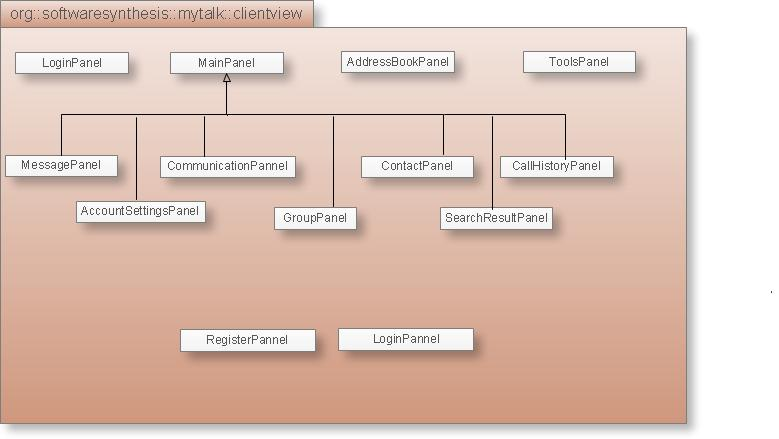
\includegraphics[width=1\textwidth]{class_gui}
  \caption{Diagramma delle classi - Architettura \texttt{mytalk.clientview}}\label{fig:sottoarchview}
\end{figure}
\clearpage

\section{Design pattern utilizzati}
In conformità con quanto stabilito nella sezione 7.2 del documento \textit{norme\_di\_progetto.3.0.pdf}, per ognuno dei \inglese{design pattern} sono riportati lo scopo e una descrizione del contesto di applicazione del \inglese{pattern} all'interno di un componente, evidenziando in particolar modo i vantaggi derivati e riportando un diagramma esemplificativo.

Per una visione d'insieme dei componenti utilizzati da un \inglese{pattern}, e dei \inglese{pattern} utilizzati da un componente, si rimanda alle sottosezioni ``Tracciamenti Componenti-Design Pattern'' e ``Tracciamenti Design Pattern-Componenti'' della sezione \vref{sec:tracciamenti}.

\subsection{Data Access Object (DAO)}\label{sec:patterndao}

\subsubsection{Scopo}
Il \inglese{pattern} DAO ha lo scopo di disaccoppiare la logica di \inglese{business} dalla logica di accesso ai dati, questo si ottiene spostando la logica di accesso ai dati dai componenti di \inglese{business} stessi ad una classe DAO ad hoc per il DBMS scelto, rendendo i componenti che implementano la \inglese{business logic} indipendenti dalla natura del dispositivo di persistenza.

Un simile approccio garantisce che un eventuale cambiamento del dispositivo di persistenza non comporti modifiche sui componenti di \inglese{business}.

\subsubsection{Componenti che lo implementano}
\begin{description}
\item{\scshape\bfseries CS01 -- Gestione database}\\
La classe DAO Data Persistance Manager, consente di isolare l'accesso alle tabelle del database dalla parte di \inglese{business logic} corrispondente alle entità TO (\textit{transfer object}), incapsulando in metodi di alto livello le operazioni sui record del database sottostante.

\begin{figure}[H]
  \centering
  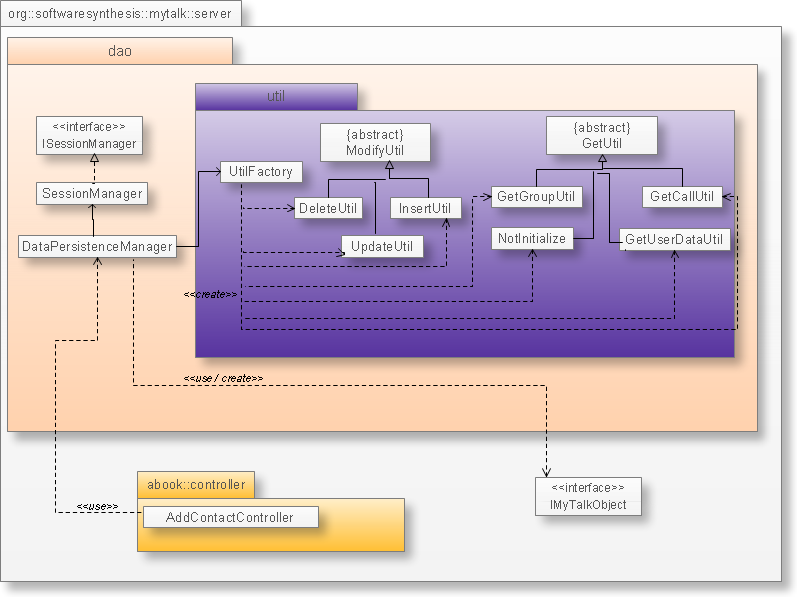
\includegraphics[width=.95\textwidth]{pattern_dao}
  \caption{Applicazione del \inglese{pattern} Data Access Object}\label{fig:dao}
\end{figure}

Operando una distinzione di questo tipo gli utenti esterni possono considerare gli oggetti che richiedono la mappatura nel database alla stregua di normali oggetti Java (POJO) senza preoccuparsi del meccanismo di persistenza dei dati.
\end{description}

\subsection{Front Controller}\label{sec:patternfacade}

\subsubsection{Scopo}
Fornire un punto d'ingresso centralizzato per la gestione delle richieste, definisce inoltre un'interfaccia di livello più alto che rende la sotto-architettura più semplice da utilizzare e riduce il numero di dipendenze funzionali fra i componenti appartenenti a sotto-architetture esterne e le classi del server.

\subsubsection{Componenti che lo implementano}
\begin{description}
  \item{\scshape\bfseries CS08 -- Front controller}\\
Questa componente della sotto-architettura server fornisce un unico punto d'accesso al sistema, andando a delegare le operazioni richieste al corrispondente controller presente in \texttt{CS07 -- Gestione controller}. La classe cosi definita è \texttt{ControllerManager}. Le componenti su cui possono interagire direttamente i controller sono: \textsf{Gestione rubrica}, \textsf{Gestione connessione}, \textsf{Gestione segreteria}, \textsf{Gestione chiamate} e \textsf{Gestione autenticazione}, come riportato nella tabella della sezione \vref{sec:cs07}.
\end{description}

\subsection{Factory Method}\label{sec:patternfactorymethod}

\subsubsection{Scopo}
Definisce un'interfaccia per la creazione di un oggetto, lasciando alle sottoclassi la decisione sulla classe concreta che deve essere istanziata e consente di deferire l'istanziazione di una classe alle sottoclassi.

\subsubsection{Componenti che lo implementano}
\begin{description}

	\item{\scshape\bfseries CS01 -- Gestione database}\\
In tale componente è la classe \texttt{dao.DataPersistanceManager} a definire dei metodi per la creazione di istanze di classi figlie di \texttt{dao.util.GetUtil} e \texttt{dao.util.ModifyUtil}.

  \item{\scshape\bfseries CS02 -- Gestione connessione}\\
Gli oggetti che intendono rappresentare connessioni sono sottotipi della classe di libreria \texttt{org.apache.catalina.websocket.StreamInbound} e vengono instanziati mediante un Factory Method nelle sottoclassi di \texttt{org.apache.catalina.websocket.WebSocketServlet}.

\begin{figure}[H]
  \centering
  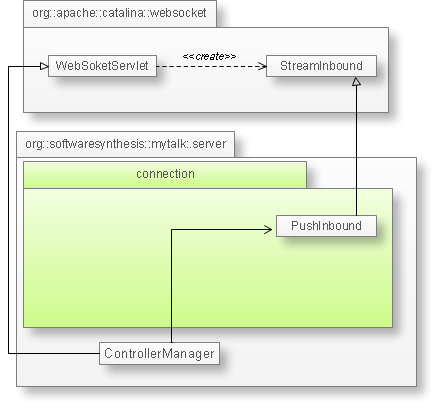
\includegraphics[width=.8\textwidth]{pattern_factorymethod}
  \caption{Applicazione del \inglese{pattern} Factory Method}\label{fig:factory_method}
\end{figure}

In particolare, la classe \texttt{ControllerManager} restituisce un oggetto che rappresenta la connessione di tipo dinamico \texttt{connection.PushInbound} che implementa il comportamento come reazione ai messaggi in ingresso facendo a sua volta \inglese{overriding} del metodo \texttt{onTextMessage(CharBuffer)}.

\end{description}

\subsection{Strategy}\label{sec:patternstrategy}

\subsubsection{Scopo}
Definisce un'interfaccia per il comportamento di un algoritmo generico, lasciando alle classi implementanti il compito di definirne la strategia d'implementazione.

\subsubsection{Componenti che lo implementano}
\begin{description}

  \item{\scshape\bfseries CS04 -- Gestione autenticazione}\\
All'interno di tale classe l'utilizzo del pattern si ha nel momento in cui è necessario definire una strategia di criptazione e decriptazione dei dati, passati dall'utente per eseguire l'autenticazione. L'interfaccia atta a definire l'algoritmo generico è \texttt{authentication.security.ISecurityStrategy} mentre una prima implementazione proposta dal team è \texttt{authentication.security.AESAlgorithm}, che definisce un algoritmo di criptazione basato su AES.

\begin{figure}[H]
  \centering
  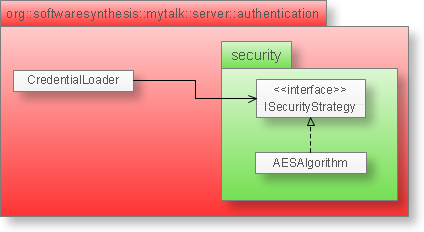
\includegraphics[width=.8\textwidth]{pattern_strategy}
  \caption{Applicazione del \inglese{pattern} Strategy}\label{fig:strategy}
\end{figure}

\end{description}

\subsection{Template Method}
\subsubsection{Scopo}
Permette di definire la struttura di un algoritmo lasciando alle sottoclassi il compito di implementarne alcuni passi specifici in modo da personalizzare il comportamento delle sottoclassi senza dover necessariamente riscrivere il codice comune a tali algoritmi.

\subsubsection{Componenti che lo implementano}

\begin{description}

  \item{\scshape\bfseries CS01 -- Gestione database}\\
In tale componente la classe \texttt{dao.uti.ModifyUtil} implementa il pattern \texttt{template method} definendo un metodo per l'esecuzione di un'operazione su \texttt{dao.DataPersistenceManager}, e lasciando l'implementazione dell'algoritmo alle classi figlie. Tali sono: \texttt{dao.uti.InsertUtil}, \texttt{dao.uti.UpdateUtil} e \texttt{dao.uti.DeleteUtil}.

Anche la classe \texttt{dao.uti.GetUtil} implementa lo stesso comportamento, lasciando alle classi figlie (\texttt{dao.uti.GetCallUtil}, \texttt{dao.uti.GetGroupUtil}, \texttt{dao.uti.GetUserUtil}, \texttt{dao.uti.NotInitialize}) il compito di definire l'algoritmo d'implementazione.

	\item{\scshape\bfseries CS04 -- Gestione autenticazione}\\
In tale componente la classe \texttt{authentication.security.AESTemplate} implementa il pattern \texttt{template method} definendo un metodo per l'esecuzione di un operazione AES. Nello specifico le operazioni possibili sono: criptazione e decriptazione. Tali sono rappresentate dalle classi figlie \texttt{authentication.security.AESEncode} e \texttt{authentication.security.AESDecode}.

	\item{\scshape\bfseries CS07 -- Gestione controller}\\
In tale componente la classe \texttt{server.AbstractController} definisce una procedura per l'esecuzione di una richiesta inoltrata da un client alg server. Tale procedura prevede di richiamare un metodo atto all'esecuzione della richiesta specifica. La procedura definita da tale metodo, secondo l'implementazione del \texttt{template method}, viene ridefinita all'interno delle classi figlie di \texttt{server.AbstractController}. Tali classi sono tutte e sole quelle contenute nella componente CS07, ossia tutti i controller del sistema.

\end{description}

\subsection{Model-View-Presenter}\label{sec:MVP}

\subsubsection{Scopo}
Il pattern architetturale \inglese{Model-View-Presenter} similmente a quanto accade per \inglese{Model-View-Controller} (MVC), ha lo scopo di mantenere separata la \inglese{business logic}, cioè la gestione dei dati secondo le regole di un determinato dominio e la loro memorizzazione in forma persistente, dalla presentazione e manipolazione mediante interfaccia utente.


\begin{figure}[H]
  \centering
  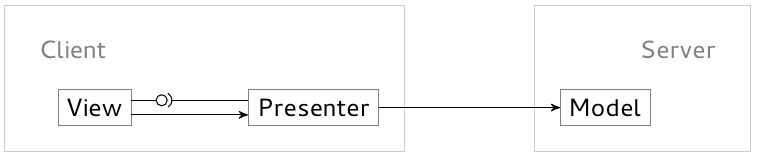
\includegraphics[width=.8\textwidth]{mvpHLdiagram}
  \caption{Diagramma ad alto livello del \inglese{pattern} MVP}\label{fig:mvpHL}
\end{figure}

\begin{figure}[H]
  \centering
  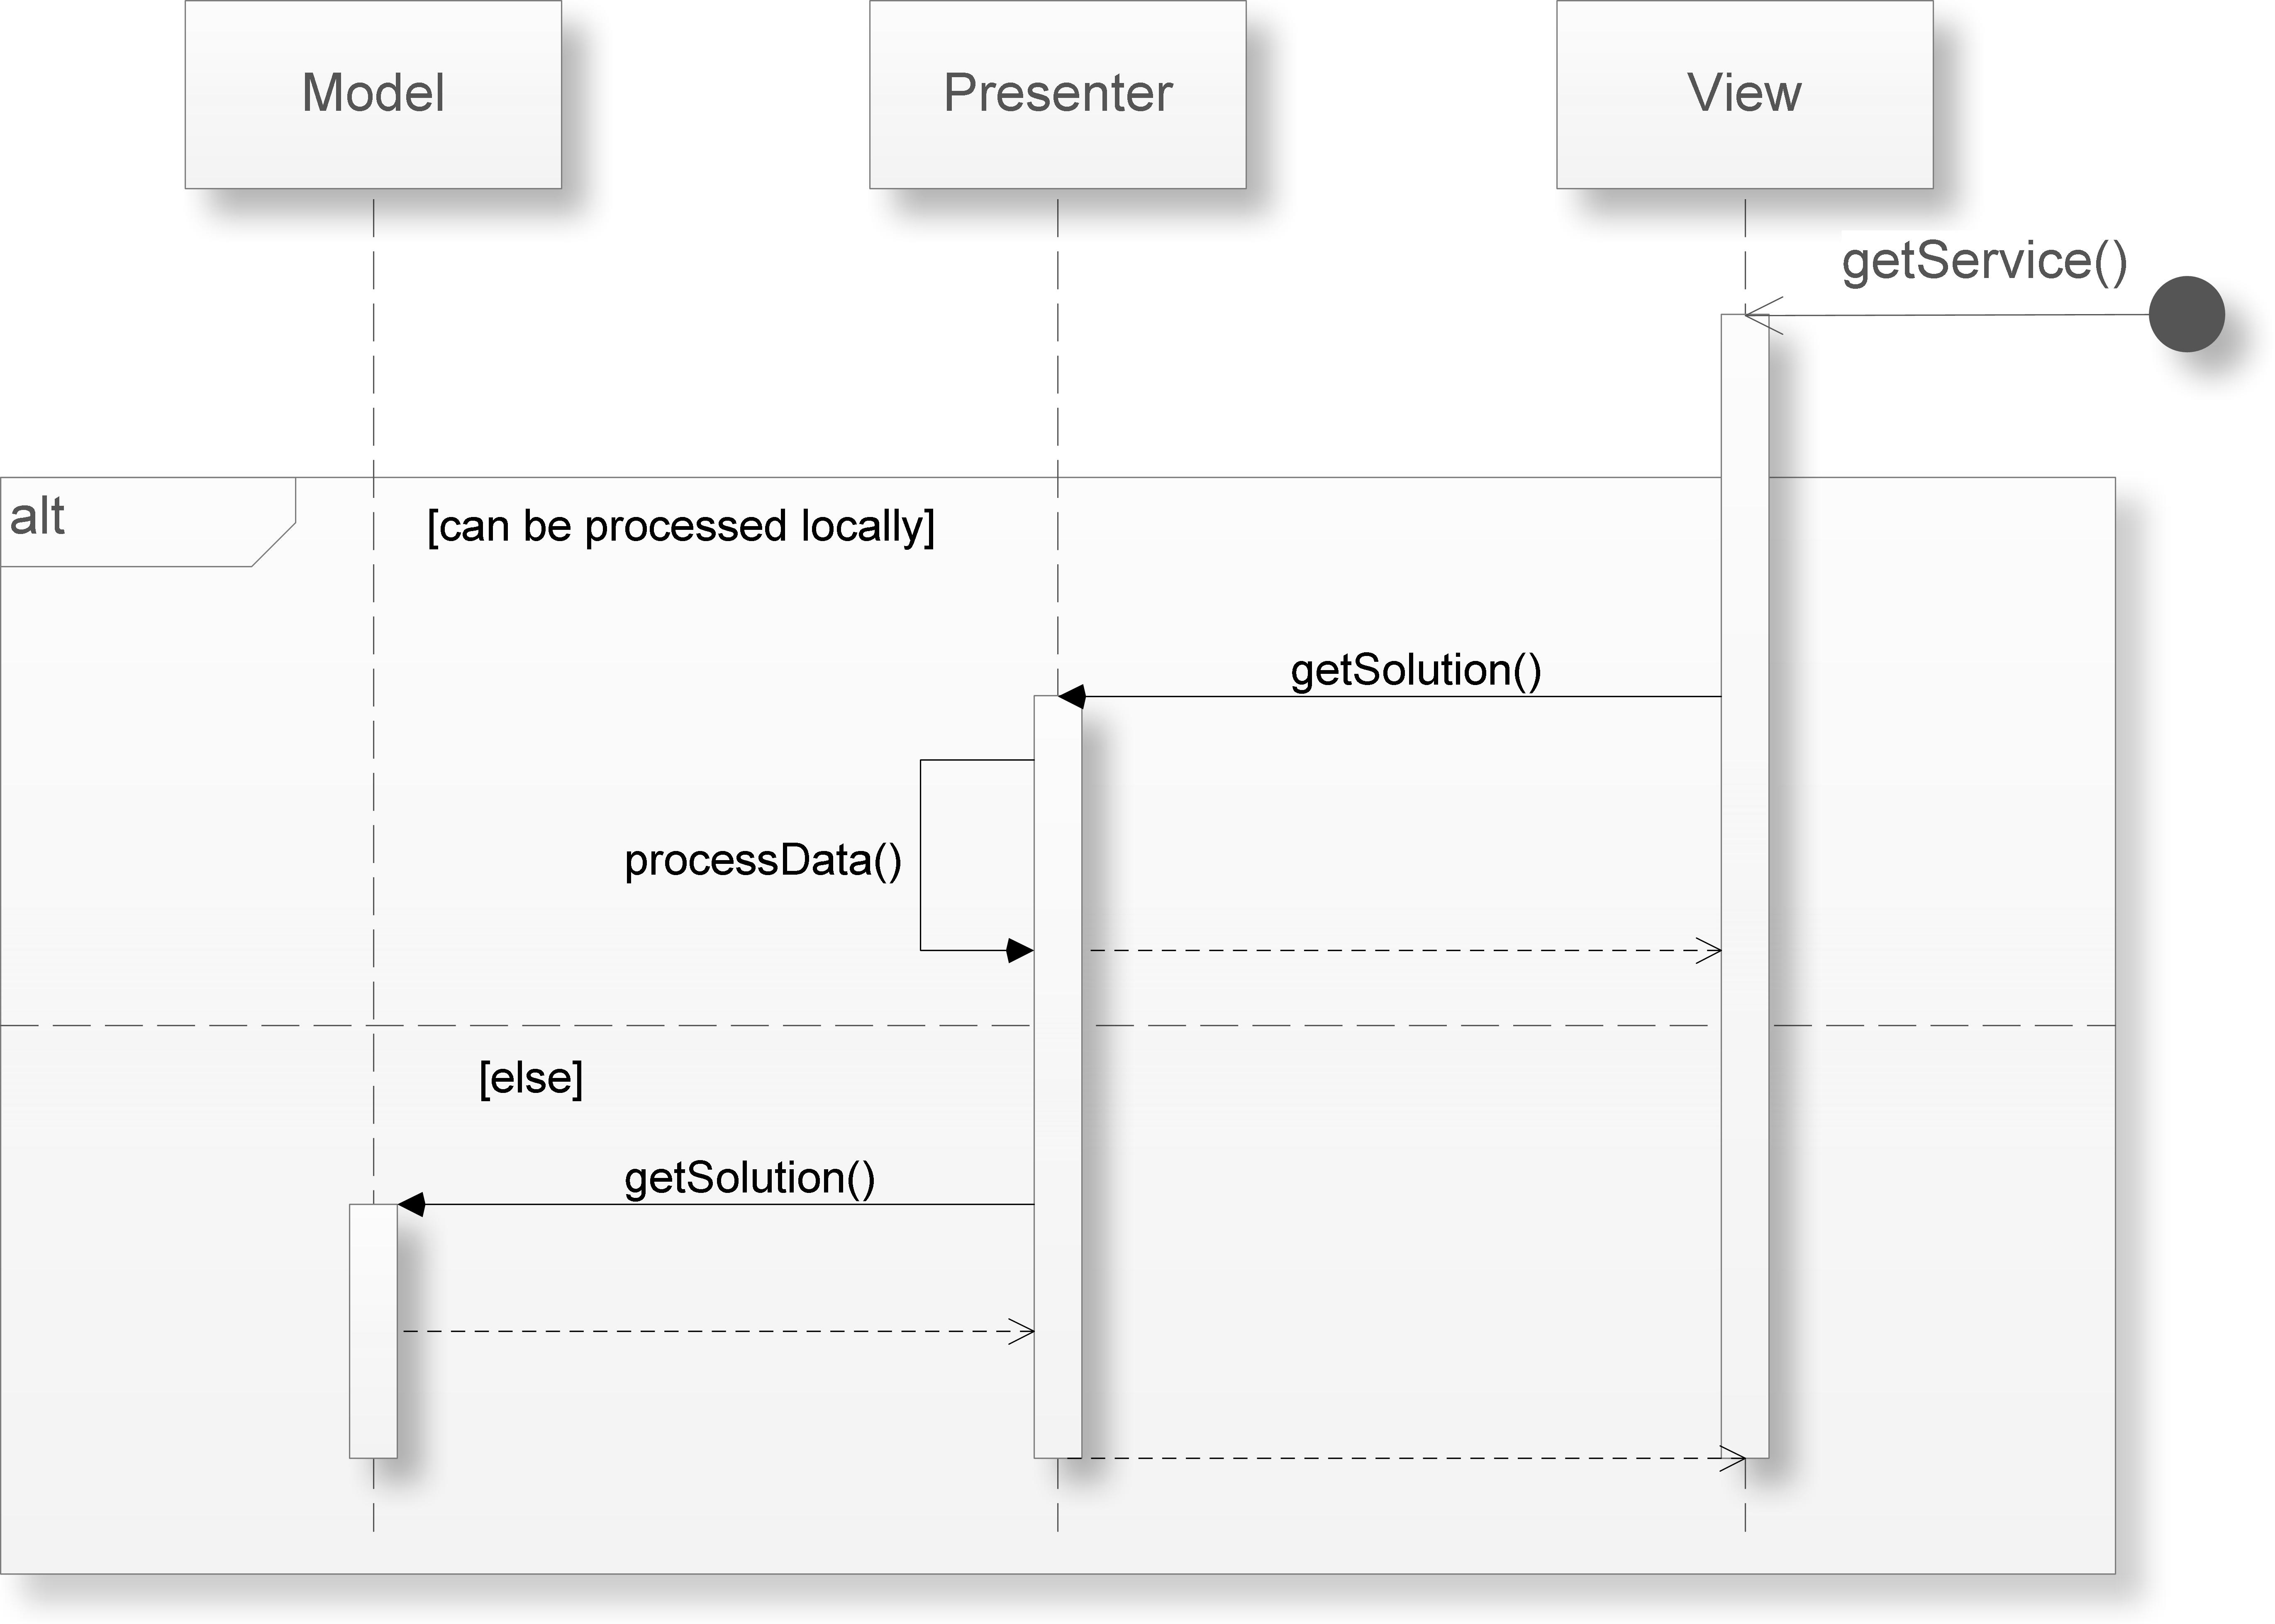
\includegraphics[width=\textwidth]{diagrammasequenzaMVP}
  \caption{Diagramma di sequenza che illustra le collaborazioni in MVP}\label{fig:mvpSD}
\end{figure}

Come si evince dal diagramma riportato in figura \ref{fig:mvpSD} le interazioni avvengono solo tra \inglese{view} e \inglese{presenter} oppure tra \inglese{presenter} e \inglese{model}, senza che avvenga mai uno scambio di dati diretto fra \inglese{model} e \inglese{view}.

Ciò si deve al fatto che la \inglese{business logic} e il modello dei dati risiedono nel server mentre il \inglese{presenter} e la \inglese{view} sono situati nel client. Quando un utente richiede un servizio tramite l'interfaccia grafica, la richiesta viene inoltrata dalla \inglese{view} al \inglese{presenter}.

Qualora quest'ultimo fosse in grado di soddisfare tale richiesta con le risorse di cui dispone, i dati sono restituiti immediatamente alla \inglese{view} senza alcun bisogno di richiedere l'intervento del server. Nel caso, invece, in cui il \inglese{presenter} non fosse in grado di servire autonomamente la \inglese{view}, interrogherebbe il server al fine di ottenere i dati da restituire alla componente grafica.

Il vantaggio di un simile schema di interazione consiste nella riduzione del traffico di rete e nel conseguente incremento delle prestazioni in termini di velocità e, di conseguenza, dell'esperienza utente in generale.

\subsubsection{Componenti che lo implementano}
MVP viene utilizzato come il \inglese{pattern} più ad alto livello del sistema: la distinzione fra \inglese{model}, \inglese{presenter} e \inglese{view} è infatti rispecchiata dalla suddivisione del sistema nelle tre sotto-architetture \texttt{server}, \texttt{clientpresenter} e \texttt{clientview}.

In generale, l'utilizzo di MVP riduce l'accoppiamento tra le sotto-architetture minimizzando le modifiche richieste a ognuno di essi come conseguenza di cambiamenti all'interno degli altri.

Inoltre i componenti di questa sotto-architettura non sono vincolati a utilizzare la rete per accedere alle informazioni che sono memorizzate sul server quando queste sono già disponibili (e possono essere elaborate) sul client, migliorando quindi l'esperienza utente.

Le componenti del sistema che prendono parte alle collaborazioni previste dal \inglese{pattern} MVP sono
\begin{description}
  \item{\scshape\bfseries CS01 -- Gestione database}\\
Componente che ha il ruolo di gestire la persistenza dei dati sul server necessaria alla memorizzazione delle entità di interesse del modello dei dati.

  \item{\textsc{\bfseries CS06 -- Gestione chiamate}, \textsc{\bfseries CS03 -- Gestione rubrica} e \textsc{\bfseries CS05 -- Gestione segreteria}}\\
Contengono le rappresentazioni delle entità della \inglese{business logic} lato server che devono essere interrogate per ricavare le informazioni necessarie ai client in forma opportuna.

  \item{\scshape\bfseries CS07 -- Gestione controller}\\
Componente del server interessato dalla ricezione delle richieste da parte dei \inglese{presenter}, recupera le informazioni di cui questi ultimi necessitano e le restituisce in forma serializzata e compatibile con il dominio applicativo dei client.

  \item{\scshape\bfseries CP04 -- Gestione comunicazione}\\
Intercetta le comunicazioni entranti verso il client a partire dal server che non hanno origine in una richiesta esplicita da parte del client come, ad esempio, gli aggiornamenti di stato dei diversi utenti o le chiamate in ingresso.
  
  \item{\scshape\bfseries CP03 -- Gestione GUI}\\
Riceve i comandi dalla vista ed è responsabile del suo aggiornamento e dell'interrogazione del server nel momento in cui i dati necessari per popolare l'interfaccia utente non siano disponibili sul client. Questo componente integra al suo interno gli oggetti \inglese{presenter} specifici per ogni vista e ne gestisce la collaborazione.

  \item{\scshape\bfseries GUI}\\
Corrisponde all'insieme delle viste ed è accessibile al \inglese{presenter} tramite le DOM API di JavaScript.
\end{description}

\subsection{Singleton}

\subsubsection{Scopo}
Il \inglese{pattern} creazionale Singleton, garantisce che una determinata classe possa essere istanziata una sola volta e di fornirne un punto di accesso globale. Questo \inglese{pattern} va utilizzato negli ambiti in cui si ha la necessità che l'accesso ad una determinata entità sia unico, in modo da permettere la gestione ottimale della risorsa stessa.

\subsubsection{Componenti che lo implementano}
\begin{description}
  \item{\scshape\bfseries CS01 -- Gestione database}\\
La classe \texttt{server.dao.SessionManager} è implementata come Singleton dal momento che si desidera che in ogni momento ne sia attiva un'unica istanza. 

\begin{figure}[H]
  \centering
  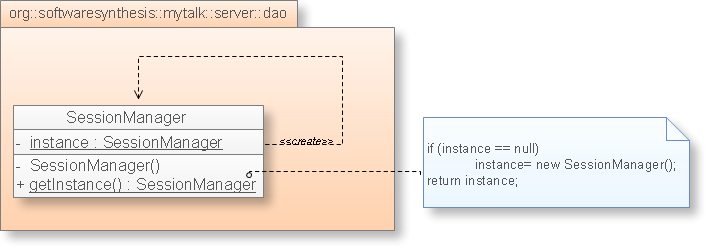
\includegraphics[width=.6\textwidth]{pattern_singleton_dao}
  \caption{Applicazione del \inglese{pattern} Singleton a \textsf{Gestione database}}\label{fig:singleton2}
\end{figure}

\end{description}
\clearpage

\section{Diagrammi delle attività}
In questa sezione saranno descritti i diagrammi di attività che rappresentano il flusso di utilizzo dei vari servizi messi a disposizione dal prodotto \caName.

\subsection{Diagramma di attività generale}

Il diagramma in figura \vref{fig:ADhome} rappresenta il flusso principale dell'applicazione \caName. L'accesso alle funzionalità del sistema è vincolato allo svolgimento con successo dell'azione di autenticazione, illustrata con maggiori dettagli nel diagramma di sotto-attività \vref{fig:ADautenticazione}.

\begin{figure}[H]
\centering
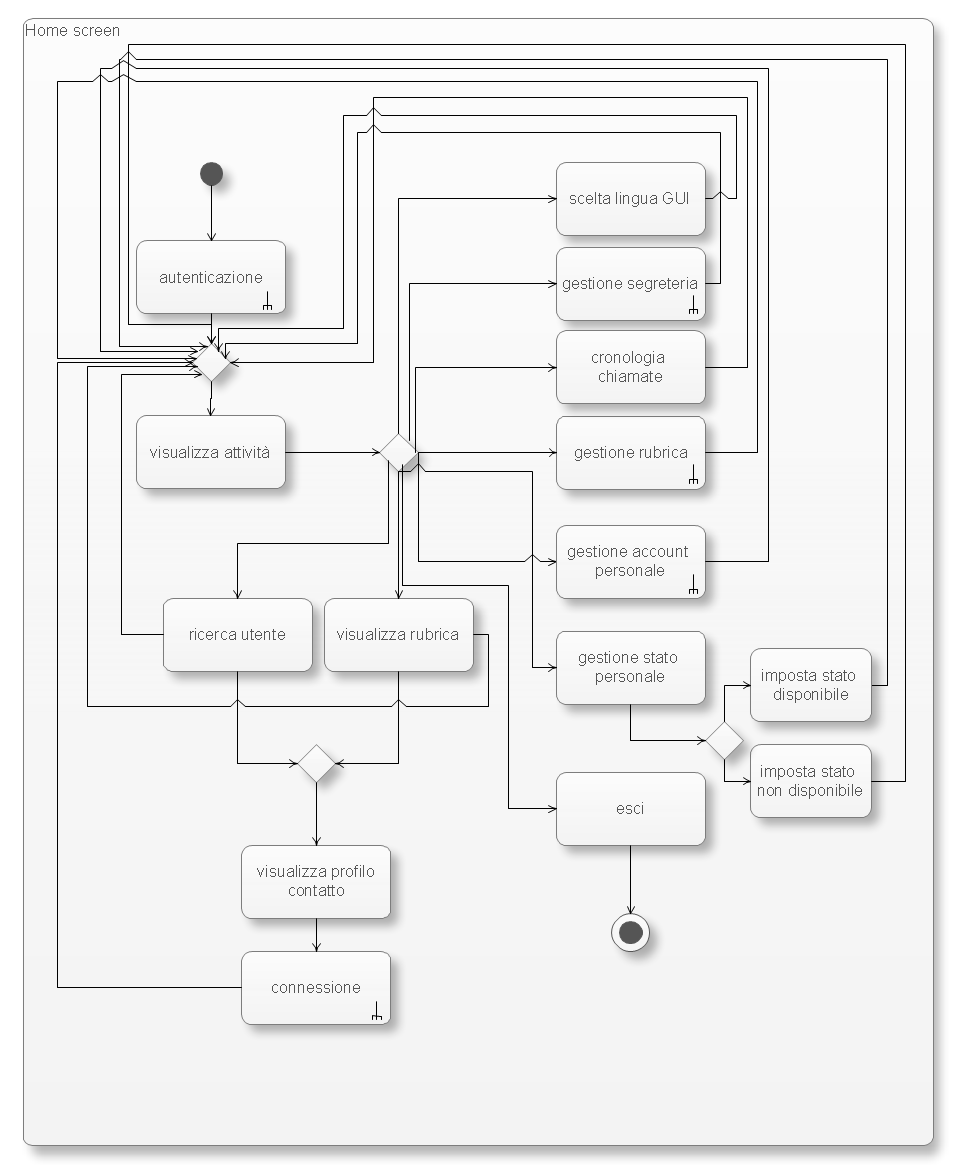
\includegraphics[width=.8\textwidth]{home}
\caption{Diagramma di attività generale che descrive l'interazione con il sistema}\label{fig:ADhome}
\end{figure}

A seguito dell'autenticazione, diviene possibile scegliere una fra le azioni di amministrazione, vale a dire
\begin{itemize}[noitemsep,nolistsep]
  \item[-] scelta lingua GUI;
  \item[-] gestione segreteria (illustrata dal diagramma \ref{fig:ADgestionesegreteria});
  \item[-] gestione rubrica (illustrata dal diagramma \ref{fig:ADgestionerubrica});
  \item[-] gestione account (illustrata dal diagramma \ref{fig:ADgestioneaccount});
  \item[-] gestione dello stato personale;
\end{itemize}
oppure di consultazione informazioni, in particolare:
\begin{itemize}[noitemsep,nolistsep]
  \item[-] visualizzazione dello storico delle chiamate;
  \item[-] visualizzazione della rubrica;
  \item[-] ricerca di un utente.
\end{itemize}

A partire infine dalla visualizzazione del profilo di un utente, cui è possibile accedere tanto tramite una ricerca quanto dall'elenco dei contatti in rubrica, è possibile dare inizio a una comunicazione (diagramma \vref{fig:ADconnessione}).

\subsection{Diagrammi di attività Autenticazione}
Il diagramma riportato in figura \vref{fig:ADautenticazione} illustra la sotto-attività di autenticazione di un utente al sistema. A partire dalla schermata iniziale è possibile inserire le proprie credenziali di accesso al sistema se ne si è provvisti, richiederle se è la prima volta che si effettua l'accesso al sistema (avviando la procedura di registrazione riportata in figura \ref{fig:ADregistrazione}) oppure recuperarle (sotto-attività in figura \vref{fig:ADrecuperopassword}).

\begin{figure}[H]
  \centering
  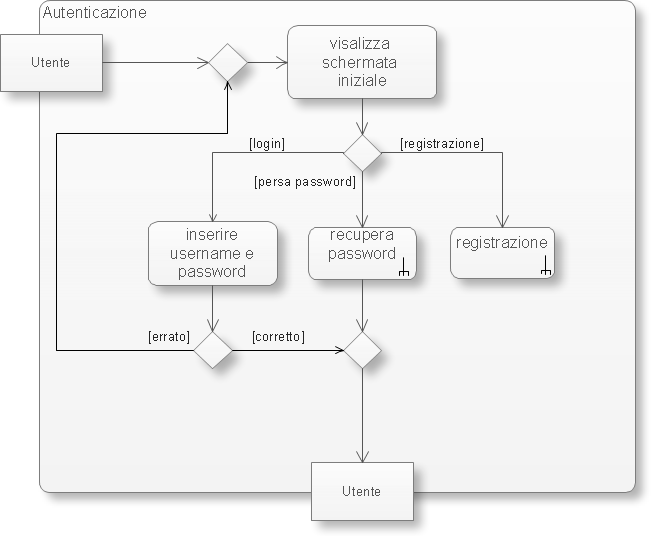
\includegraphics[width=.8\textwidth]{autent}
  \caption{Diagramma di attività relativo all'autententicazione}\label{fig:ADautenticazione}
\end{figure}

\subsubsection{Diagramma di attività Registrazione}
In dettaglio, la registrazione di un utente al sistema (fig.~\vref{fig:ADregistrazione}) prevede l'inserimento di una serie di dati alcuni dei quali obbligatori (indirizzo email, password, domanda segreta e relativa risposta) e altri facoltativi (nome, cognome e immagine del profilo). Al termine della procedura di registrazione l'utente dispone di un account personale e delle credenziali di accesso allo stesso.

\begin{figure}[H]
  \centering
  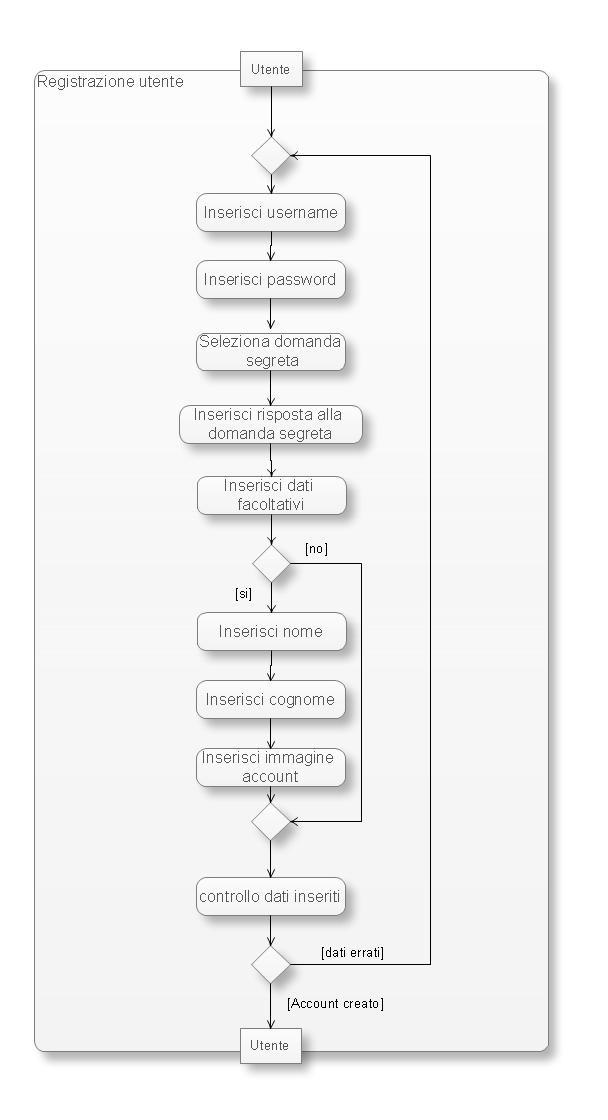
\includegraphics[width=.6\textwidth]{registrazione}
  \caption{Diagramma di attività relativo alla registrazione}\label{fig:ADregistrazione}
\end{figure}

\subsubsection{Diagramma di attività Recupero password}
Il recupero della password (fig.~\vref{fig:ADrecuperopassword}) prevede invece l'inserimento dell'email, la visualizzazione della domanda segreta impostata in fase di creazione dell'account e l'inserimento della relativa risposta. In caso di risposta corretta si ha il termine della sotto-attività con l'invio dei dati richiesti via email, in caso contrario la procedura deve essere ripetuta.

\begin{figure}[H]
  \centering
  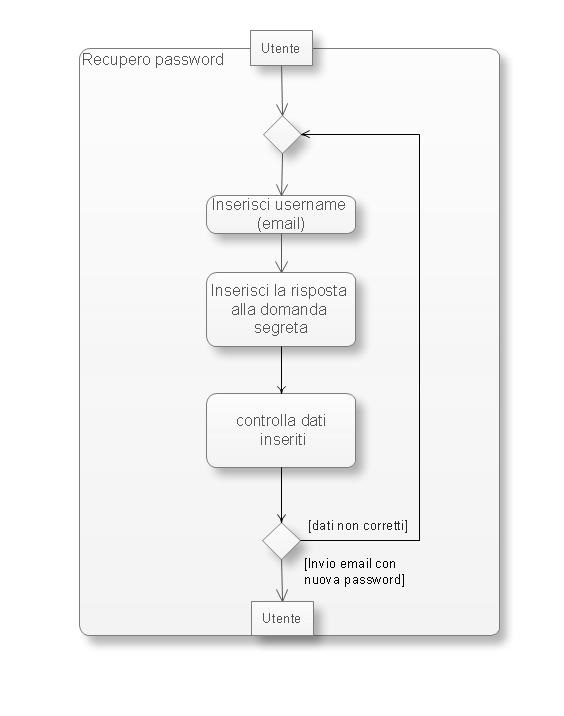
\includegraphics[width=.6\textwidth]{recPass}
  \caption{Diagramma di attività relativo al recupero della password}\label{fig:ADrecuperopassword}
\end{figure}

\subsection{Diagramma di attività Gestione rubrica}
La sotto-attività di gestione (diagramma in fig.~\vref{fig:ADgestionerubrica}) della rubrica prevede l'accesso a due classi di azioni, a seconda che sia o meno richiesta da parte dell'utente una conferma esplicita per il completamento dell'attività.

In particolare, la prima categoria di azioni comprende:
\begin{itemize}[noitemsep,nolistsep]
  \item[-] l'aggiunta di un contatto alla rubrica;
  \item[-] l'ordinamento della rubrica;
  \item[-] l'eliminazione di un contatto;
  \item[-] la ricerca di un contatto;
  \item[-] l'inserimento di un contatto in un gruppo;
\end{itemize}
mentre la seconda categoria raggruppa azioni quali:
\begin{itemize}[noitemsep,nolistsep]
  \item[-] l'eliminazione di un gruppo;
  \item[-] la modifica di un gruppo;
  \item[-] l'importazione della rubrica da un file locale in formato XML;
  \item[-] l'esportazione della rubrica personale in un file XML.
\end{itemize}

La risposta affermativa alla domanda di conferma in seguito alla scelta di un'azione della seconda categoria porta alla conclusione della sotto-attività, mentre una risposta negativa comporta la scelta di una nuova azione amministrativa.

\begin{figure}[H]
  \centering
  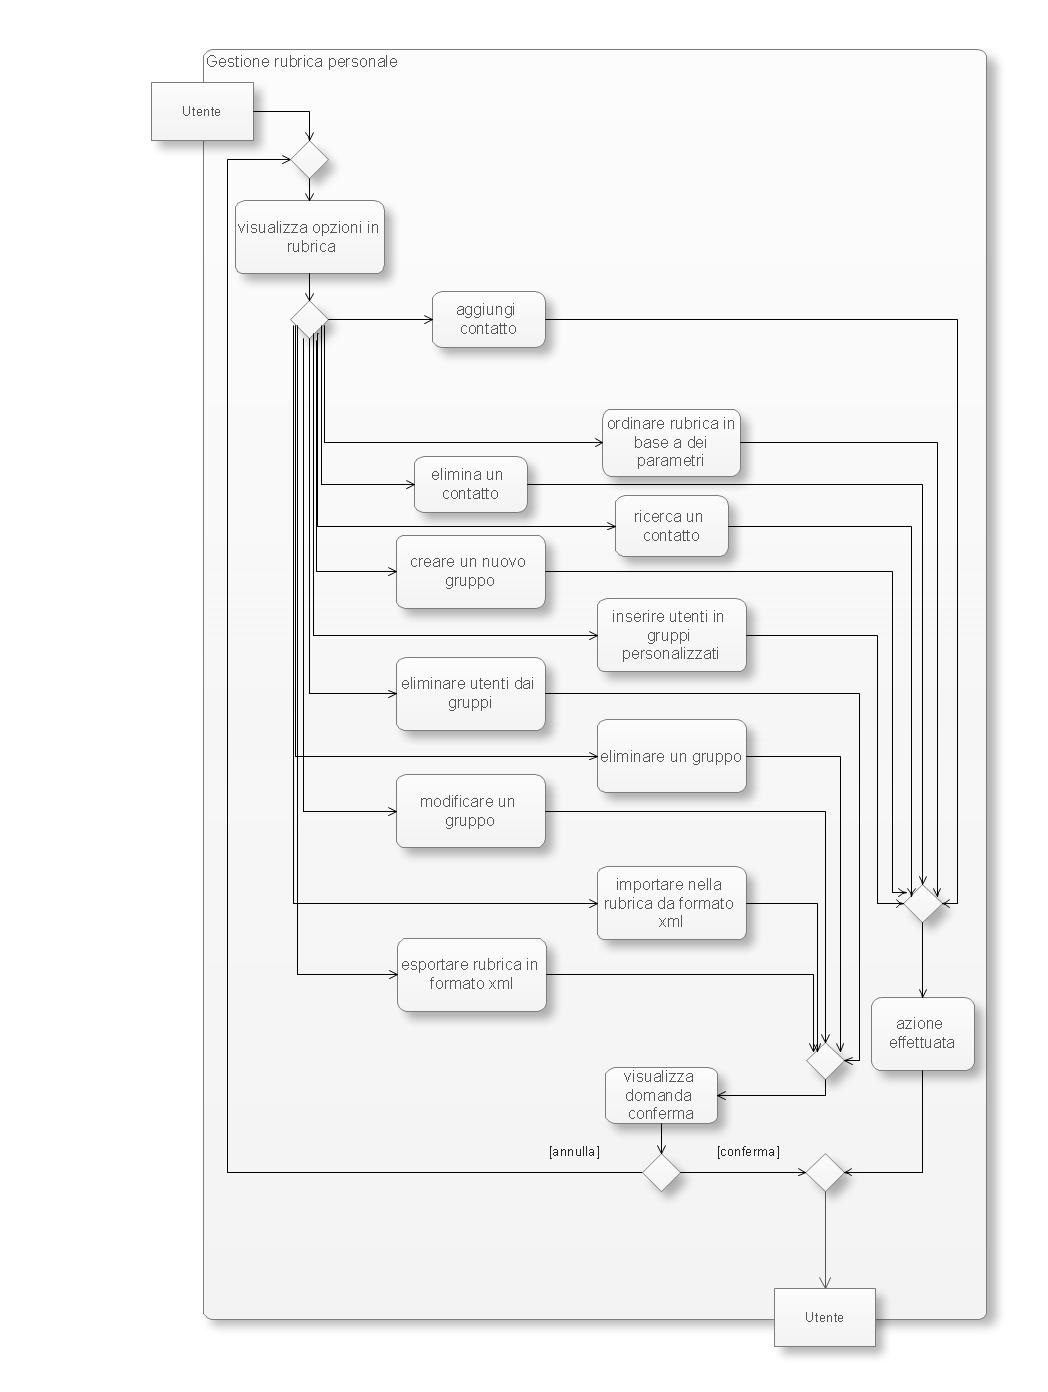
\includegraphics[width=.8\textwidth]{gestRubrica}
  \caption{Diagramma di attività relativo alla gestione della rubrica personale}\label{fig:ADgestionerubrica}
\end{figure}

\subsection{Diagramma di attività Gestione account personale}
La gestione dell'account personale (fig.~\vref{fig:ADgestioneaccount}) comporta in primo luogo la visualizzazione di una schermata che mette a disposizione le operazioni disponibili, quindi la scelta di una di queste ultime. Le azioni che possono essere effettuate sono, in particolare:
\begin{itemize}[noitemsep,nolistsep]
  \item[-] modifica della password utente;
  \item[-] modifica dei dati anagrafici;
  \item[-] modifica dell'immagine del profilo;
  \item[-] modifica della domanda segreta e/o della relativa risposta per il recupero della password.
\end{itemize}

Al termine dell'operazione è prevista la visualizzazione di una domanda di conferma e, in caso di risposta affermativa da parte dell'utente, la modifica va a buon fine. In caso contrario, l'operazione non sortisce alcun effetto e si ritorna alla possibilità di scegliere l'azione amministrativa da effettuare.

\begin{figure}[H]
  \centering
  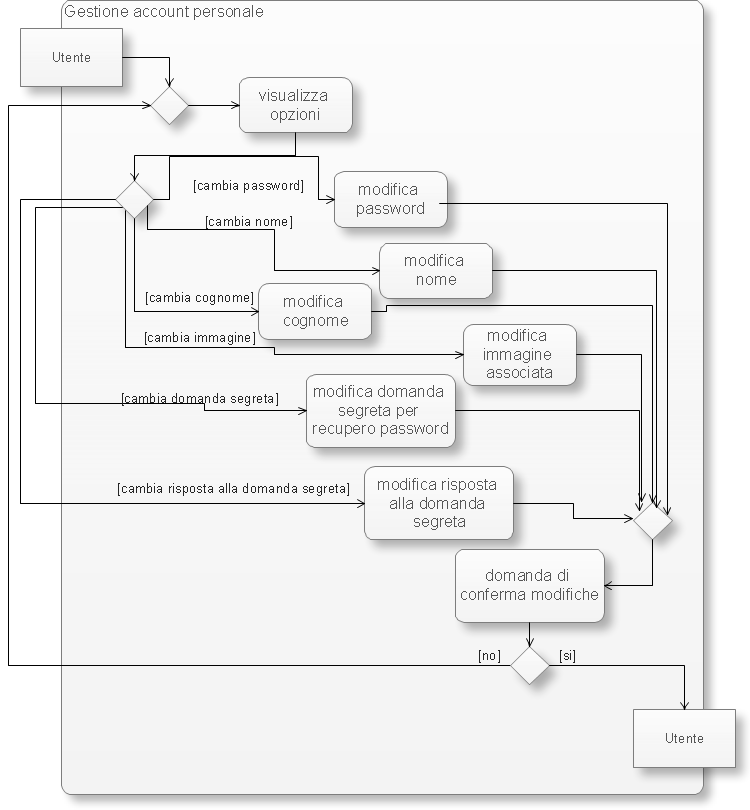
\includegraphics[width=.8\textwidth]{gestAccount}
  \caption{Diagramma di attività relativo alla gestione dei dati dell'account personale}\label{fig:ADgestioneaccount}
\end{figure}

\subsection{Diagramma di attività Gestione segreteria}
La gestione della segreteria prevede la scelta fra le seguenti azioni:
\begin{itemize}[noitemsep,nolistsep]
 \item[-] ascoltare un messaggio della segreteria;
 \item[-] cancellare un messaggio;
 \item[-] impostare lo stato (ascoltato/non ascoltato) di un messaggio;
\end{itemize}

Compiere una di queste azioni comporta l'uscita dalla sotto-attività ma l'esecuzione di più di una di queste azioni in sequenza è comunque possibile grazie al \inglese{merge} antecedente l'azione ``Visualizza attività'' nel diagramma di attività generale riportato in figura \vref{fig:ADhome}.

\begin{figure}[H]
  \centering
 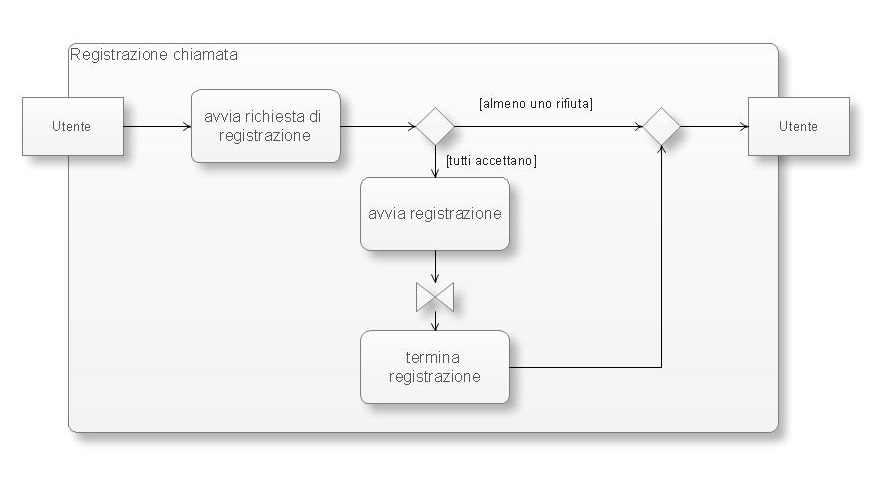
\includegraphics[width=.8\textwidth]{regChiamata}
  \caption{Diagramma di attività relativo alla gestione della segretria}\label{fig:ADgestionesegreteria}
\end{figure}

\subsection{Diagrammi di attività Connessione}
L'utente ha inoltre la possibilità di connettersi con altri utenti tramite l'attività di connessione.

Come si evince dal diagramma riportato in figura \vref{fig:ADconnessione}, la comunicazione con un utente dipende intrinsecamente dallo stato in cui si trova: se questo è \inglese{offline} oppure \inglese{online} ma occupato, può essere raggiunto in maniera indiretta solo tramite la segreteria telefonica (diagramma \ref{fig:ADmessegreteria}), mentre se l'utente è disponibile può essere contattato immediatamente.

\begin{figure}[H]
  \centering
  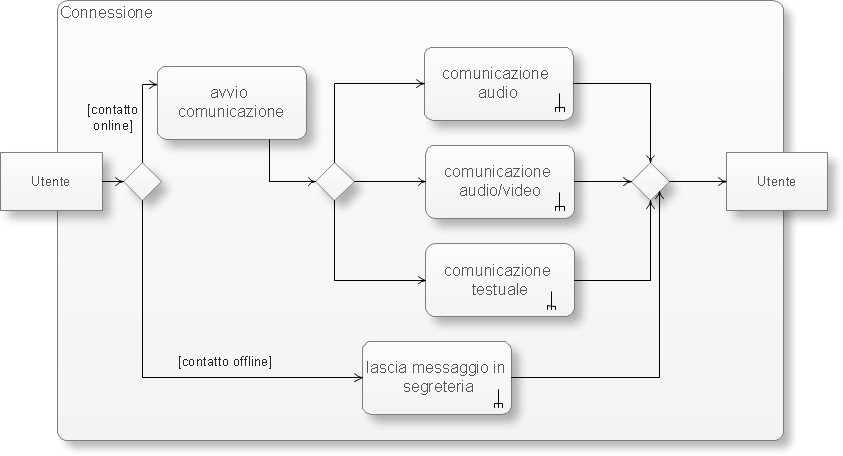
\includegraphics[width=.8\textwidth]{connessione}
  \caption{Diagramma di attività relativo alla connessione}\label{fig:ADconnessione}
\end{figure}

Esistono tre tipologie di comunicazione a seconda del mezzo utilizzato:
\begin{itemize}[noitemsep,nolistsep]
  \item[-] audio (illustrata nel diagramma in fig.~\ref{fig:ADcomaudio});
  \item[-] audio/video (diagramma in fig.~\ref{fig:ADcomaudiovideo});
  \item[-] testuale (diagramma in fig.~\ref{fig:ADcomtestuale});
\end{itemize}


Tutte e tre le tipologie di connessione prevedono la condivisione di risorse secondo le modalità riportate in figura \ref{fig:ADcondrisorse}. Inoltre, nel corso di una comunicazione di tipo audio oppure audio/video è possibile registrare una chiamata secondo le modalità riportate in figura \ref{fig:ADregistrachiamata}, nonché visualizzare le statistiche sulla comunicazione corrente (diagramma in fig.~\vref{fig:ADstatistiche}).

\subsubsection{Diagramma di attività Comunicazione audio}
La comunicazione audio (fig.~\vref{fig:ADcomaudio}) prevede la possibilità svolgimento di più azioni in parallelo, in particolare la registrazione, la condivisione di risorse, una comunicazione testuale e la visualizzazione delle statistiche sulla comunicazione in corso. Inoltre, a discrezione dell'utente, una comunicazione audio può essere promossa in una comunicazione audio/video oppure può essere estesa a nuovi partecipanti.

\begin{figure}[H]
  \centering
  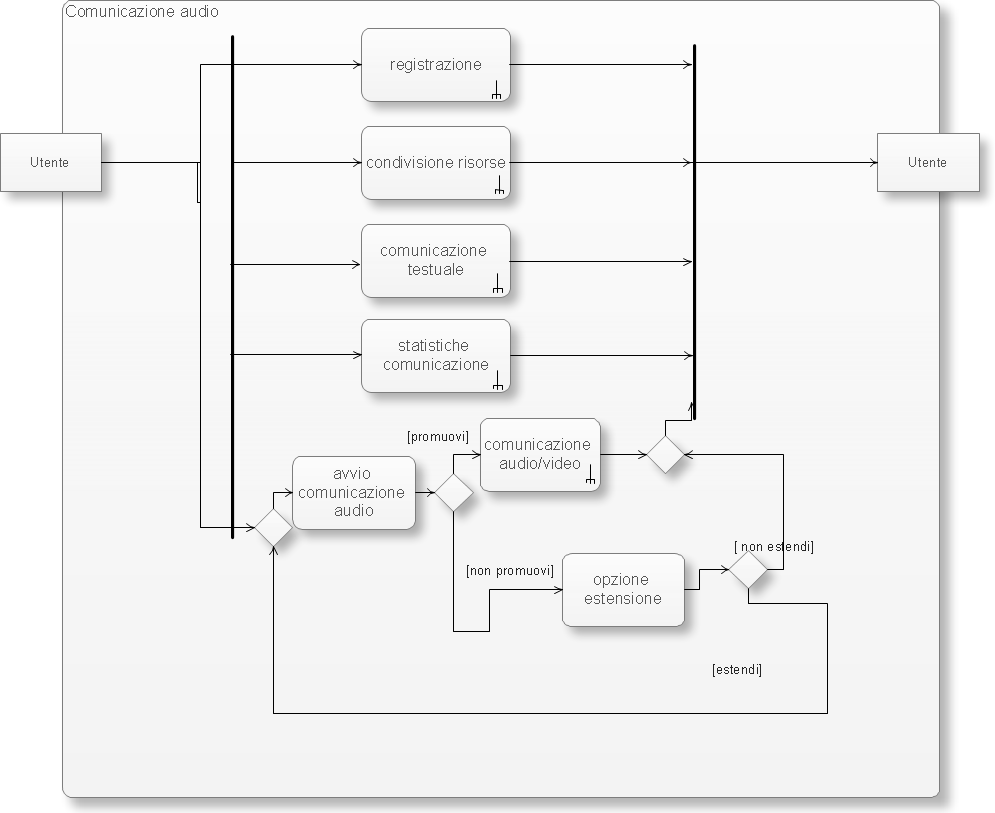
\includegraphics[width=.8\textwidth]{comAudio}
  \caption{Diagramma di attività relativo alla comunicazione audio}\label{fig:ADcomaudio}
\end{figure}

\subsubsection{Diagramma di attività Comunicazione audio/video}
La comunicazione audio/video (fig.~\vref{fig:ADcomaudiovideo}) prevede la possibilità svolgimento di più azioni in parallelo, in particolare la registrazione, la condivisione di risorse, una comunicazione testuale e la visualizzazione delle statistiche sulla comunicazione in corso. Inoltre, a discrezione dell'utente, una comunicazione audio/video può essere declassata in una comunicazione audio semplice oppure può essere estesa a nuovi partecipanti.

\begin{figure}[H]
  \centering
  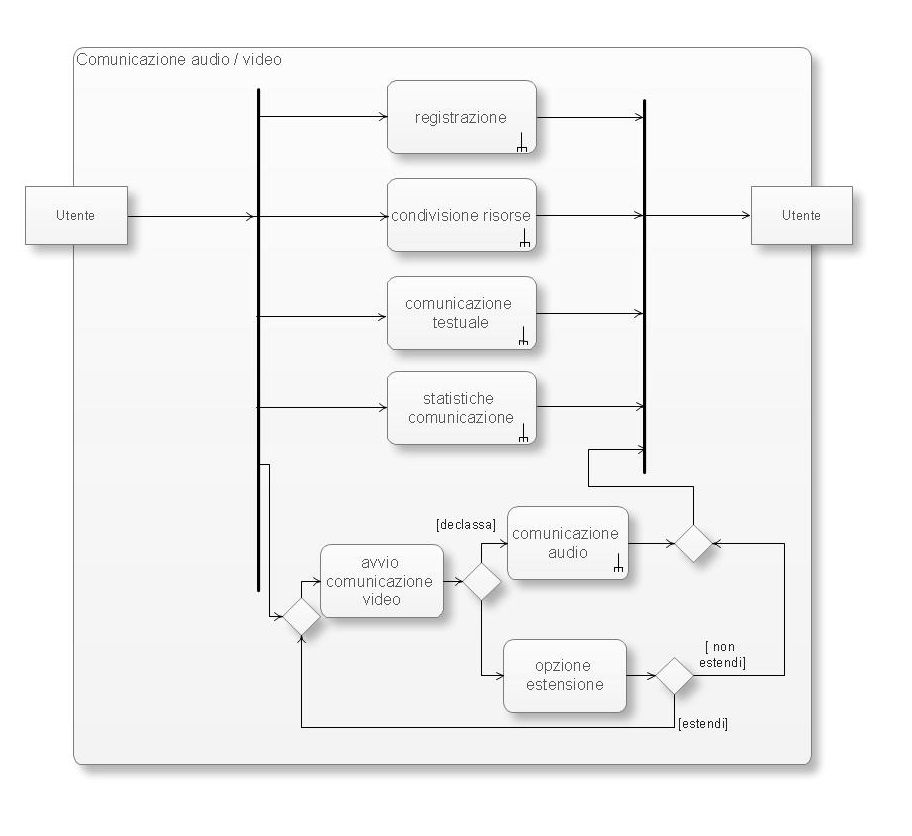
\includegraphics[width=.8\textwidth]{comAudioVideo}
  \caption{Diagramma di attività relativo alla comunicazione audio/video}\label{fig:ADcomaudiovideo}
\end{figure}

\subsubsection{Diagramma di attività Comunicazione testuale}
La comunicazione testuale, come illustrato dal diagramma riportato in figura \vref{fig:ADcomtestuale} può avvenire in parallelo con una condivisione di risorse, può essere promossa a comunicazione audio o audio/video e può essere estesa a più partecipanti. Non è prevista, durante una comunicazione testuale, la possibilità di visualizzare statistiche sulla comunicazione o di registrare la stessa in forma persistente.

\begin{figure}[H]
  \centering
  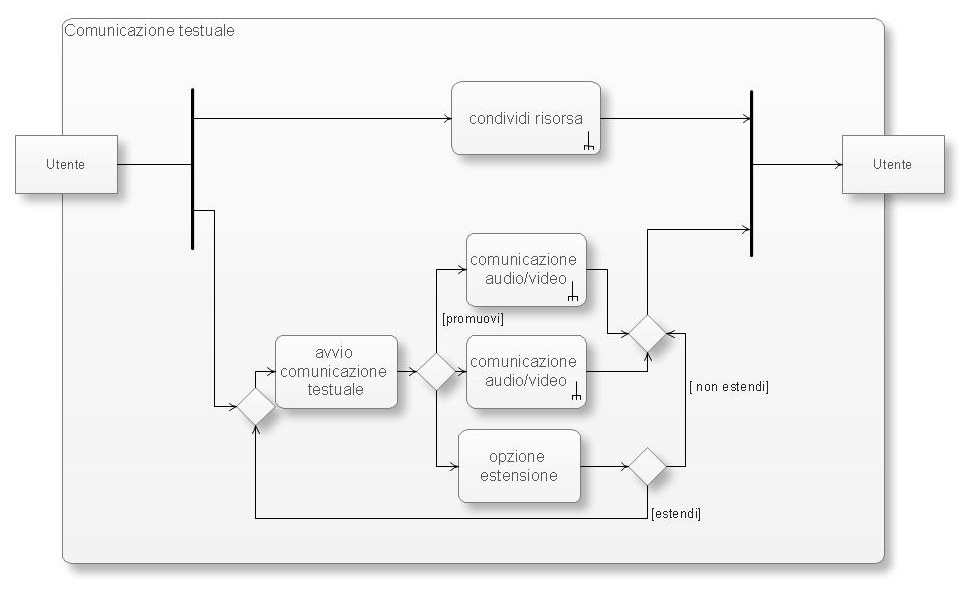
\includegraphics[width=.8\textwidth]{comTestuale}
  \caption{Diagramma di attività relativo alla comunicazione testuale}\label{fig:ADcomtestuale}
\end{figure}

\subsubsection{Diagramma di attività Condivisione di risorse}
La sotto-attività di condivisione (fig.~\vref{fig:ADcomtestuale}) di risorse comporta la possibilità di scegliere se condividere un file PDF, un file oppure lo schermo con gli altri partecipanti ad una comunicazione audio, audio/video oppure testuale.

\begin{figure}[H]
  \centering
  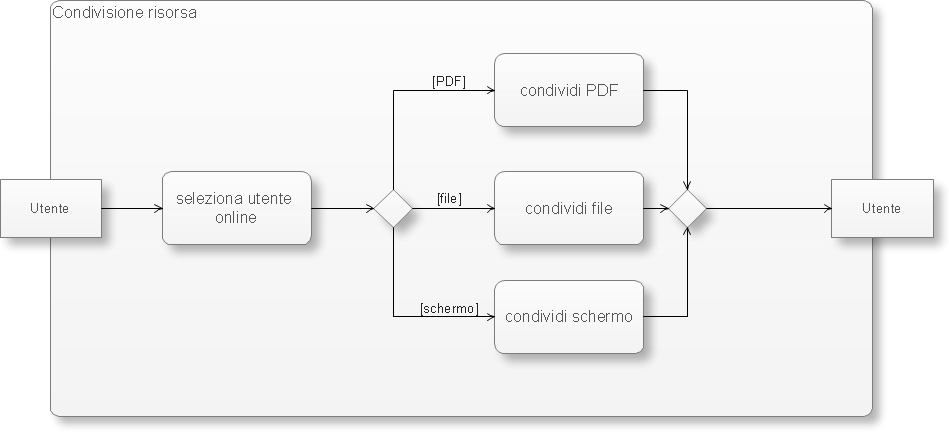
\includegraphics[width=.8\textwidth]{condRisorse}
  \caption{Diagramma di attività relativo alla condivisione di risorse}\label{fig:ADcondrisorse}
\end{figure}

\subsubsection{Diagramma di attività Registrazione chiamata}
La registrazione di una chiamata (fig.~\vref{fig:ADregistrachiamata}), sotto-attività cui è possibile accedere solo durante una comunicazione audio oppure audio/video, comporta innanzitutto l'inoltro di una richiesta di registrazione agli altri partecipanti della chiamata. Se si ottiene il consenso da parte di tutti, la registrazione ha inizio e prosegue fino a che non viene esplicitamente terminata. Se invece almeno uno degli utenti coinvolti non dà il proprio consenso alla registrazione, questa non può avere luogo.

\begin{figure}[H]
  \centering
  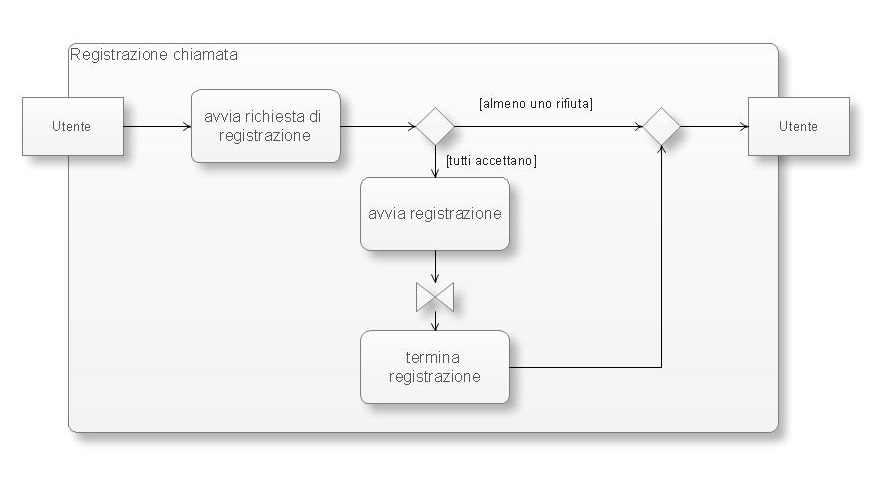
\includegraphics[width=.8\textwidth]{regChiamata}
  \caption{Diagramma di attività relativo alla registrazione della chiamata}\label{fig:ADregistrachiamata}
\end{figure}

\subsubsection{Diagramma di attività Statistiche comunicazione}
Nel corso di una comunicazione multimediale è possibile visualizzare una serie di informazioni (fig.~\vref{fig:ADstatistiche})fra cui:
\begin{itemize}[noitemsep,nolistsep]
  \item[-] il numero di byte inviati e ricevuti;
  \item[-] la velocità di trasmissione;
  \item[-] la latenza della connessione;
  \item[-] il numero di fps (nel caso delle sole comunicazioni video).
\end{itemize}

\begin{figure}[H]
  \centering
  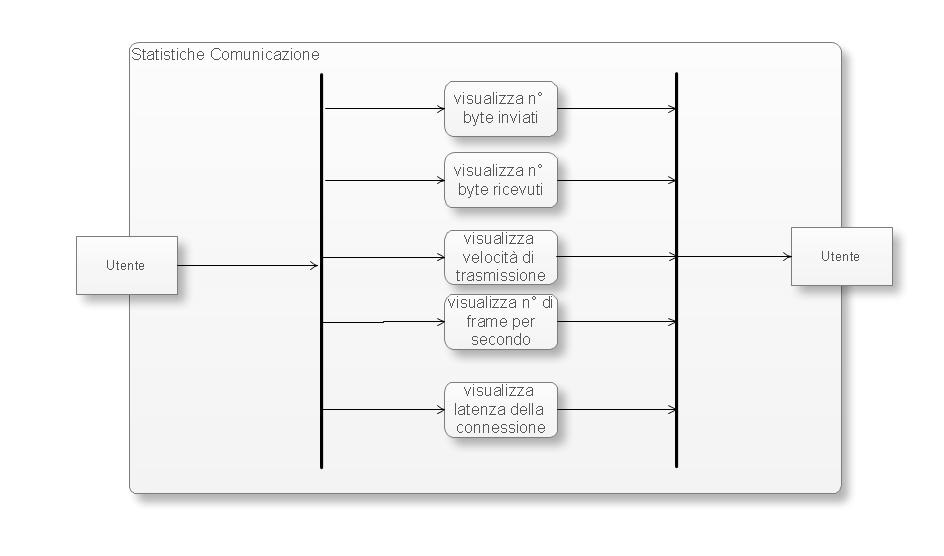
\includegraphics[width=.8\textwidth]{statistCom}
  \caption{Diagramma di attività relativo alla visualizzazione delle statistiche della comunicazione}\label{fig:ADstatistiche}
\end{figure}

\subsubsection{Diagramma di attività Messaggio in segreteria}
In conclusione, si ricorda che è possibile lasciare un messaggio nella segreteria di un determinato contatto se non presente in linea nel momento in cui desideriamo comunicare con lui \ref{fig:ADmessegreteria}. I messaggi che possono essere lasciati in segreteria possono essere costituiti da una sola traccia audio oppure da una traccia audio e da una traccia video.

\begin{figure}[H]
  \centering
  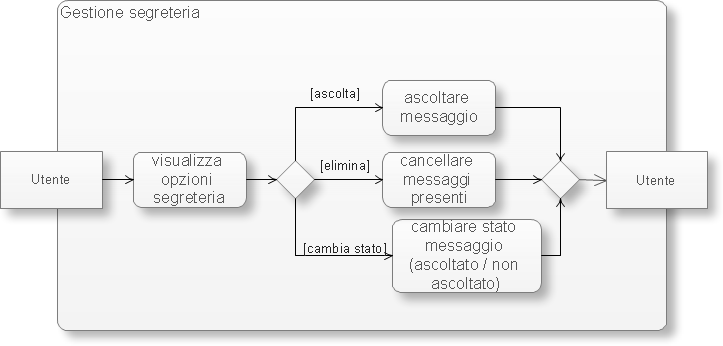
\includegraphics[width=.8\textwidth]{segreteria}
  \caption{Diagramma di attività relativo alla memorizzazione di un messaggio in segreteria}\label{fig:ADmessegreteria}
\end{figure}
\clearpage

\section{Tracciamenti}\label{sec:tracciamenti}
Nella seguente sezione vengono proposti tutti i tracciamenti eseguiti mediante il sistema \manager. I tracciamenti proposti sono giustificati dalle seguenti due motivazioni:

\begin{itemize}
	\item Dimostrare il soddisfacimento per necessità e sufficienza della corrispondenza tra gli elementi tracciati (e.g. un componente deve rispondere necessariamente alle esigenze di uno o più requisiti, tali insomma che ne giustifichino l'esistenza. D'altro canto è richiesto che ogni requisito definito in fase d'analisi sia soddisfatto e risolto da almeno un componente).
	\item dare una lettura generale delle varie: componenti, requisiti, \inglese{design pattern} e classi.
\end{itemize}

\newpage\section{Diagrammi dei casi d'uso}

\subsection{UC1: Login e registrazione}
\begin{figure}[H]
\begin{center}
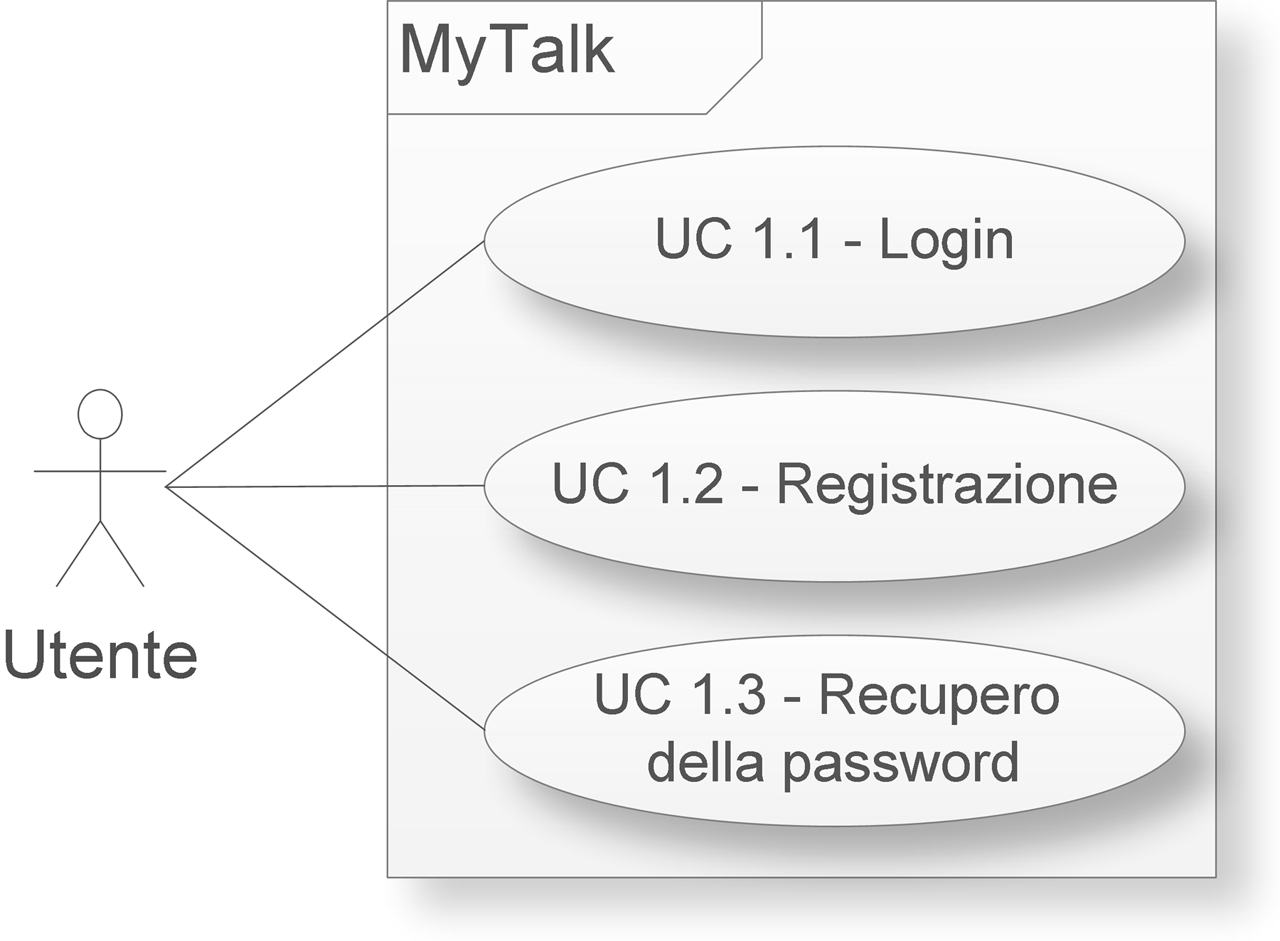
\includegraphics[width=.8\textwidth]{UC1}
\caption{}\label{fig:}
\end{center}
\end{figure}
\begin{description}
\item{\scshape\bfseries Attori principali:}Utente.
\item{\scshape\bfseries Scopo e descrizione:} L'utente può effettuare l'accesso al sistema mediante la procedura di autenticazione se registrato (UC1.1), recuperare la password dimenticata (UC1.3) oppure può provvedere alla propria registrazione (UC1.2), quindi effettuare successivamente l'accesso al sistema (UC1.1).
\item{\scshape\bfseries Precondizione:} Il sistema MyTalk è attivo e funzionante, le infrastrutture di rete sono attive.
\item{\scshape\bfseries Postcondizione:} L'utente si trova in uno di questi casi: ha avviato la procedura per l'autenticazione al sistema (UC1.1), oppure ha avviato la procedura per per la registrazione nel sistema (UC1.2), oppure ha avviato la procedura per il recupero della password dimenticata (UC1.3).
\item{\scshape\bfseries Illustrazione scenario principale:} L'utente può decidere di avviare la procedura di autenticazione al sistema (UC1.1), altrimenti se non ricorda le credenziali, può avviare la procedura per il recupero della password (UC1.3). Invece se l'utente sa di non essere registrato nel sistema, può avviare la procedura di registrazione (UC1.2).
\end{description}

\subsection{UC1.1: Login utente}
\begin{figure}[H]
\begin{center}
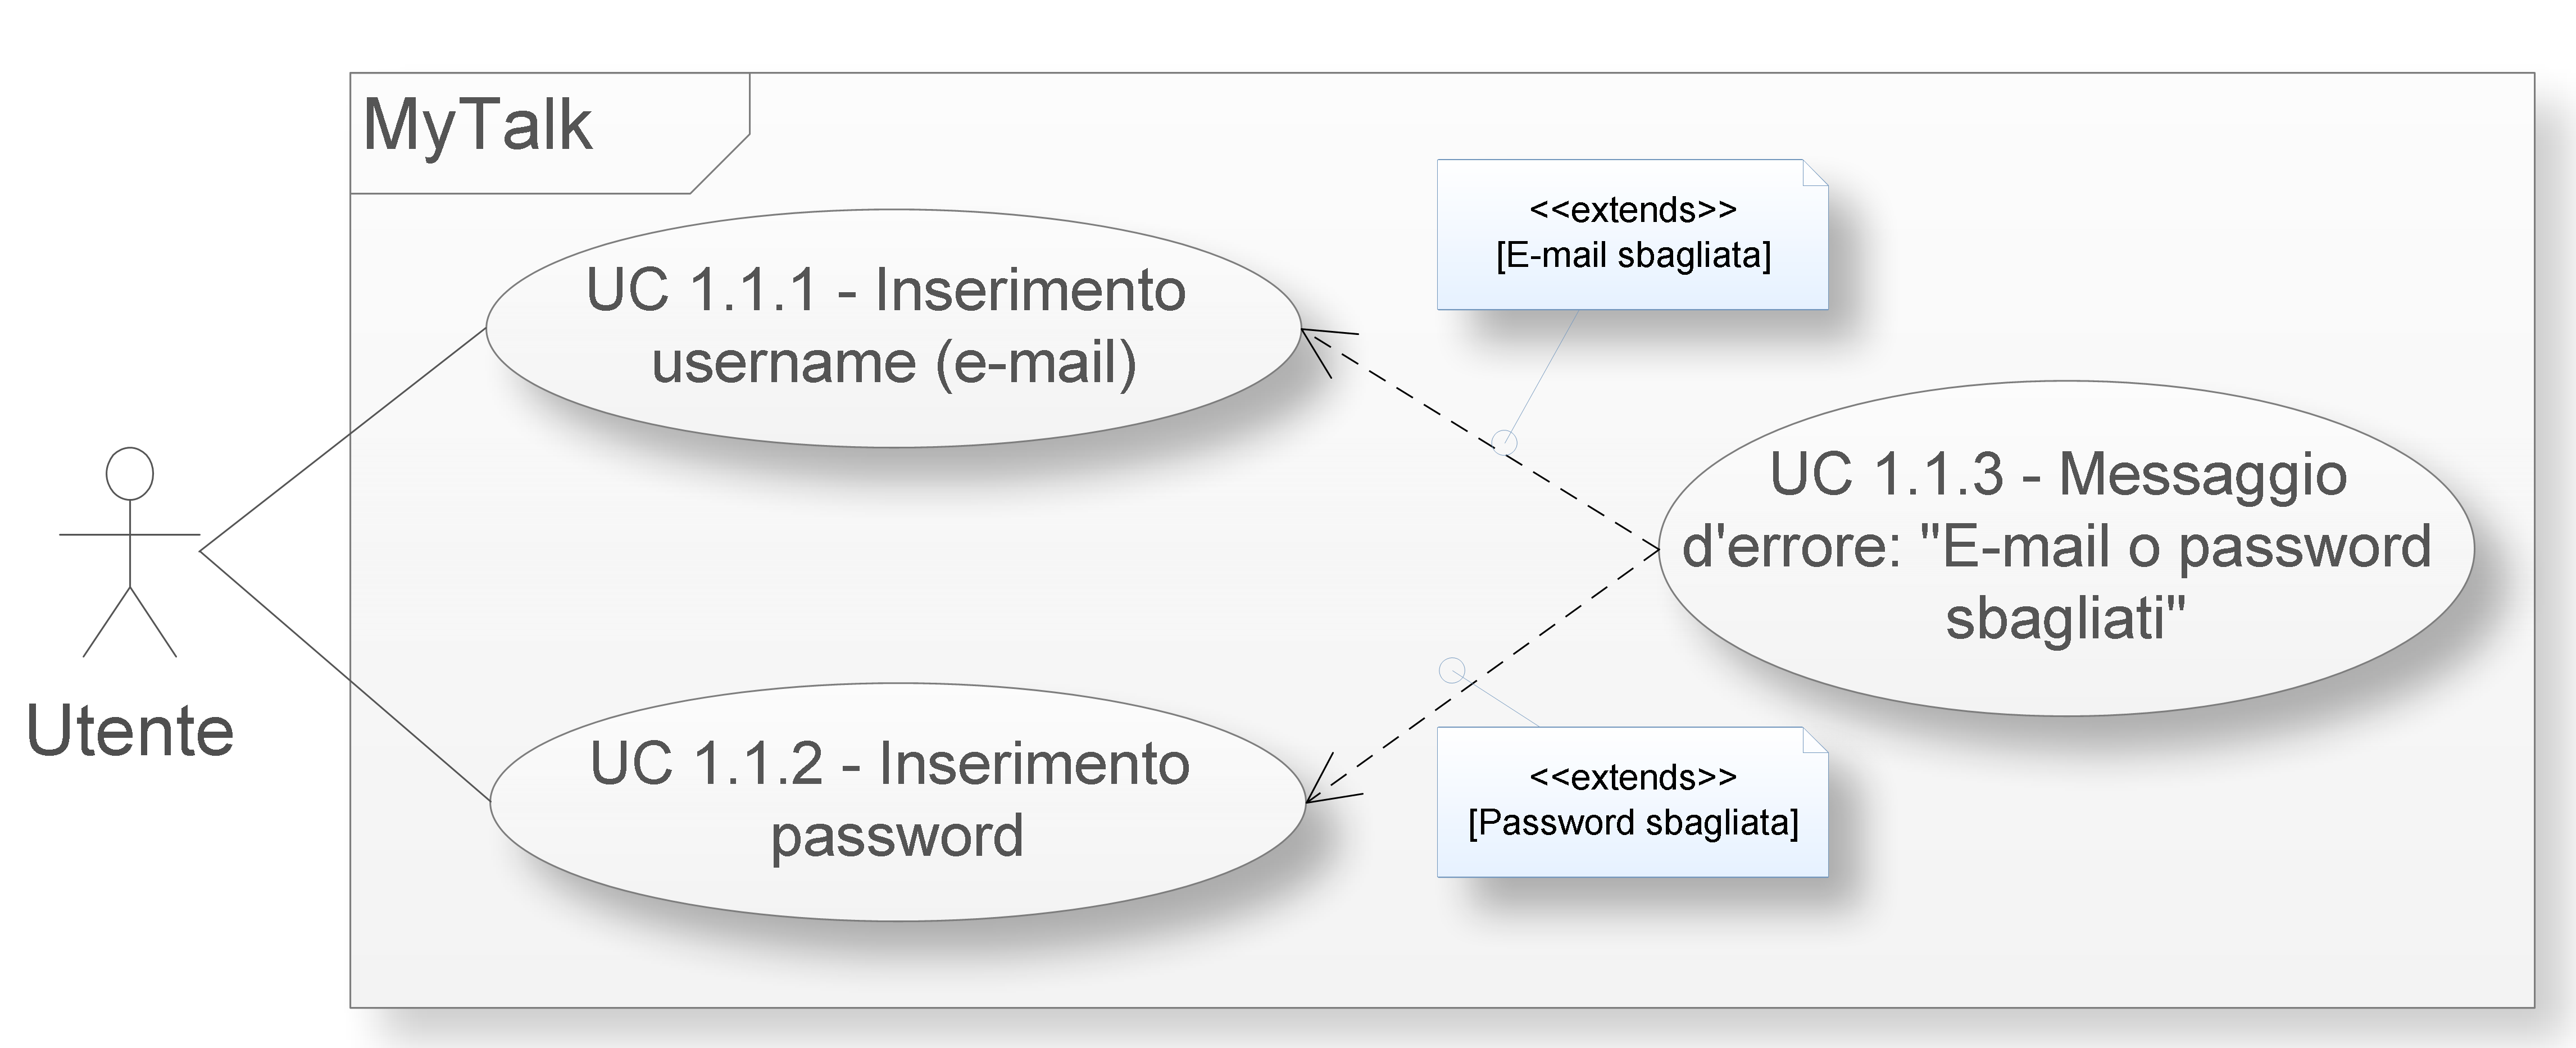
\includegraphics[width=.8\textwidth]{UC1-1}
\caption{}\label{fig:}
\end{center}
\end{figure}
\begin{description}
\item{\scshape\bfseries Attori principali:}Utente.
\item{\scshape\bfseries Scopo e descrizione:} L'utente si autentica per accedere al sistema MyTalk
\item{\scshape\bfseries Precondizione:} L'utente (generico) visualizza la schermata iniziale e il sistema è pronto.
\item{\scshape\bfseries Postcondizione:} L'utente è autenticato nel sistema
\item{\scshape\bfseries Illustrazione scenario principale:} L'utente inserisce username (UC1.1.1) e password (UC1.1.2) corretti e conferma.
\item{\scshape\bfseries Illustrazione scenario alternativo:} L'utente ha inserito dati non corretti: il sistema lo notifica con un errore unico (UC1.1.3) e rimane in attesa di una correzione. (Non vengono visualizzati due errori separati ma un errore unico generico per aumentare la sicurezza).
\end{description}

\subsection{UC1.2: Registrazione}
\begin{figure}[H]
\begin{center}
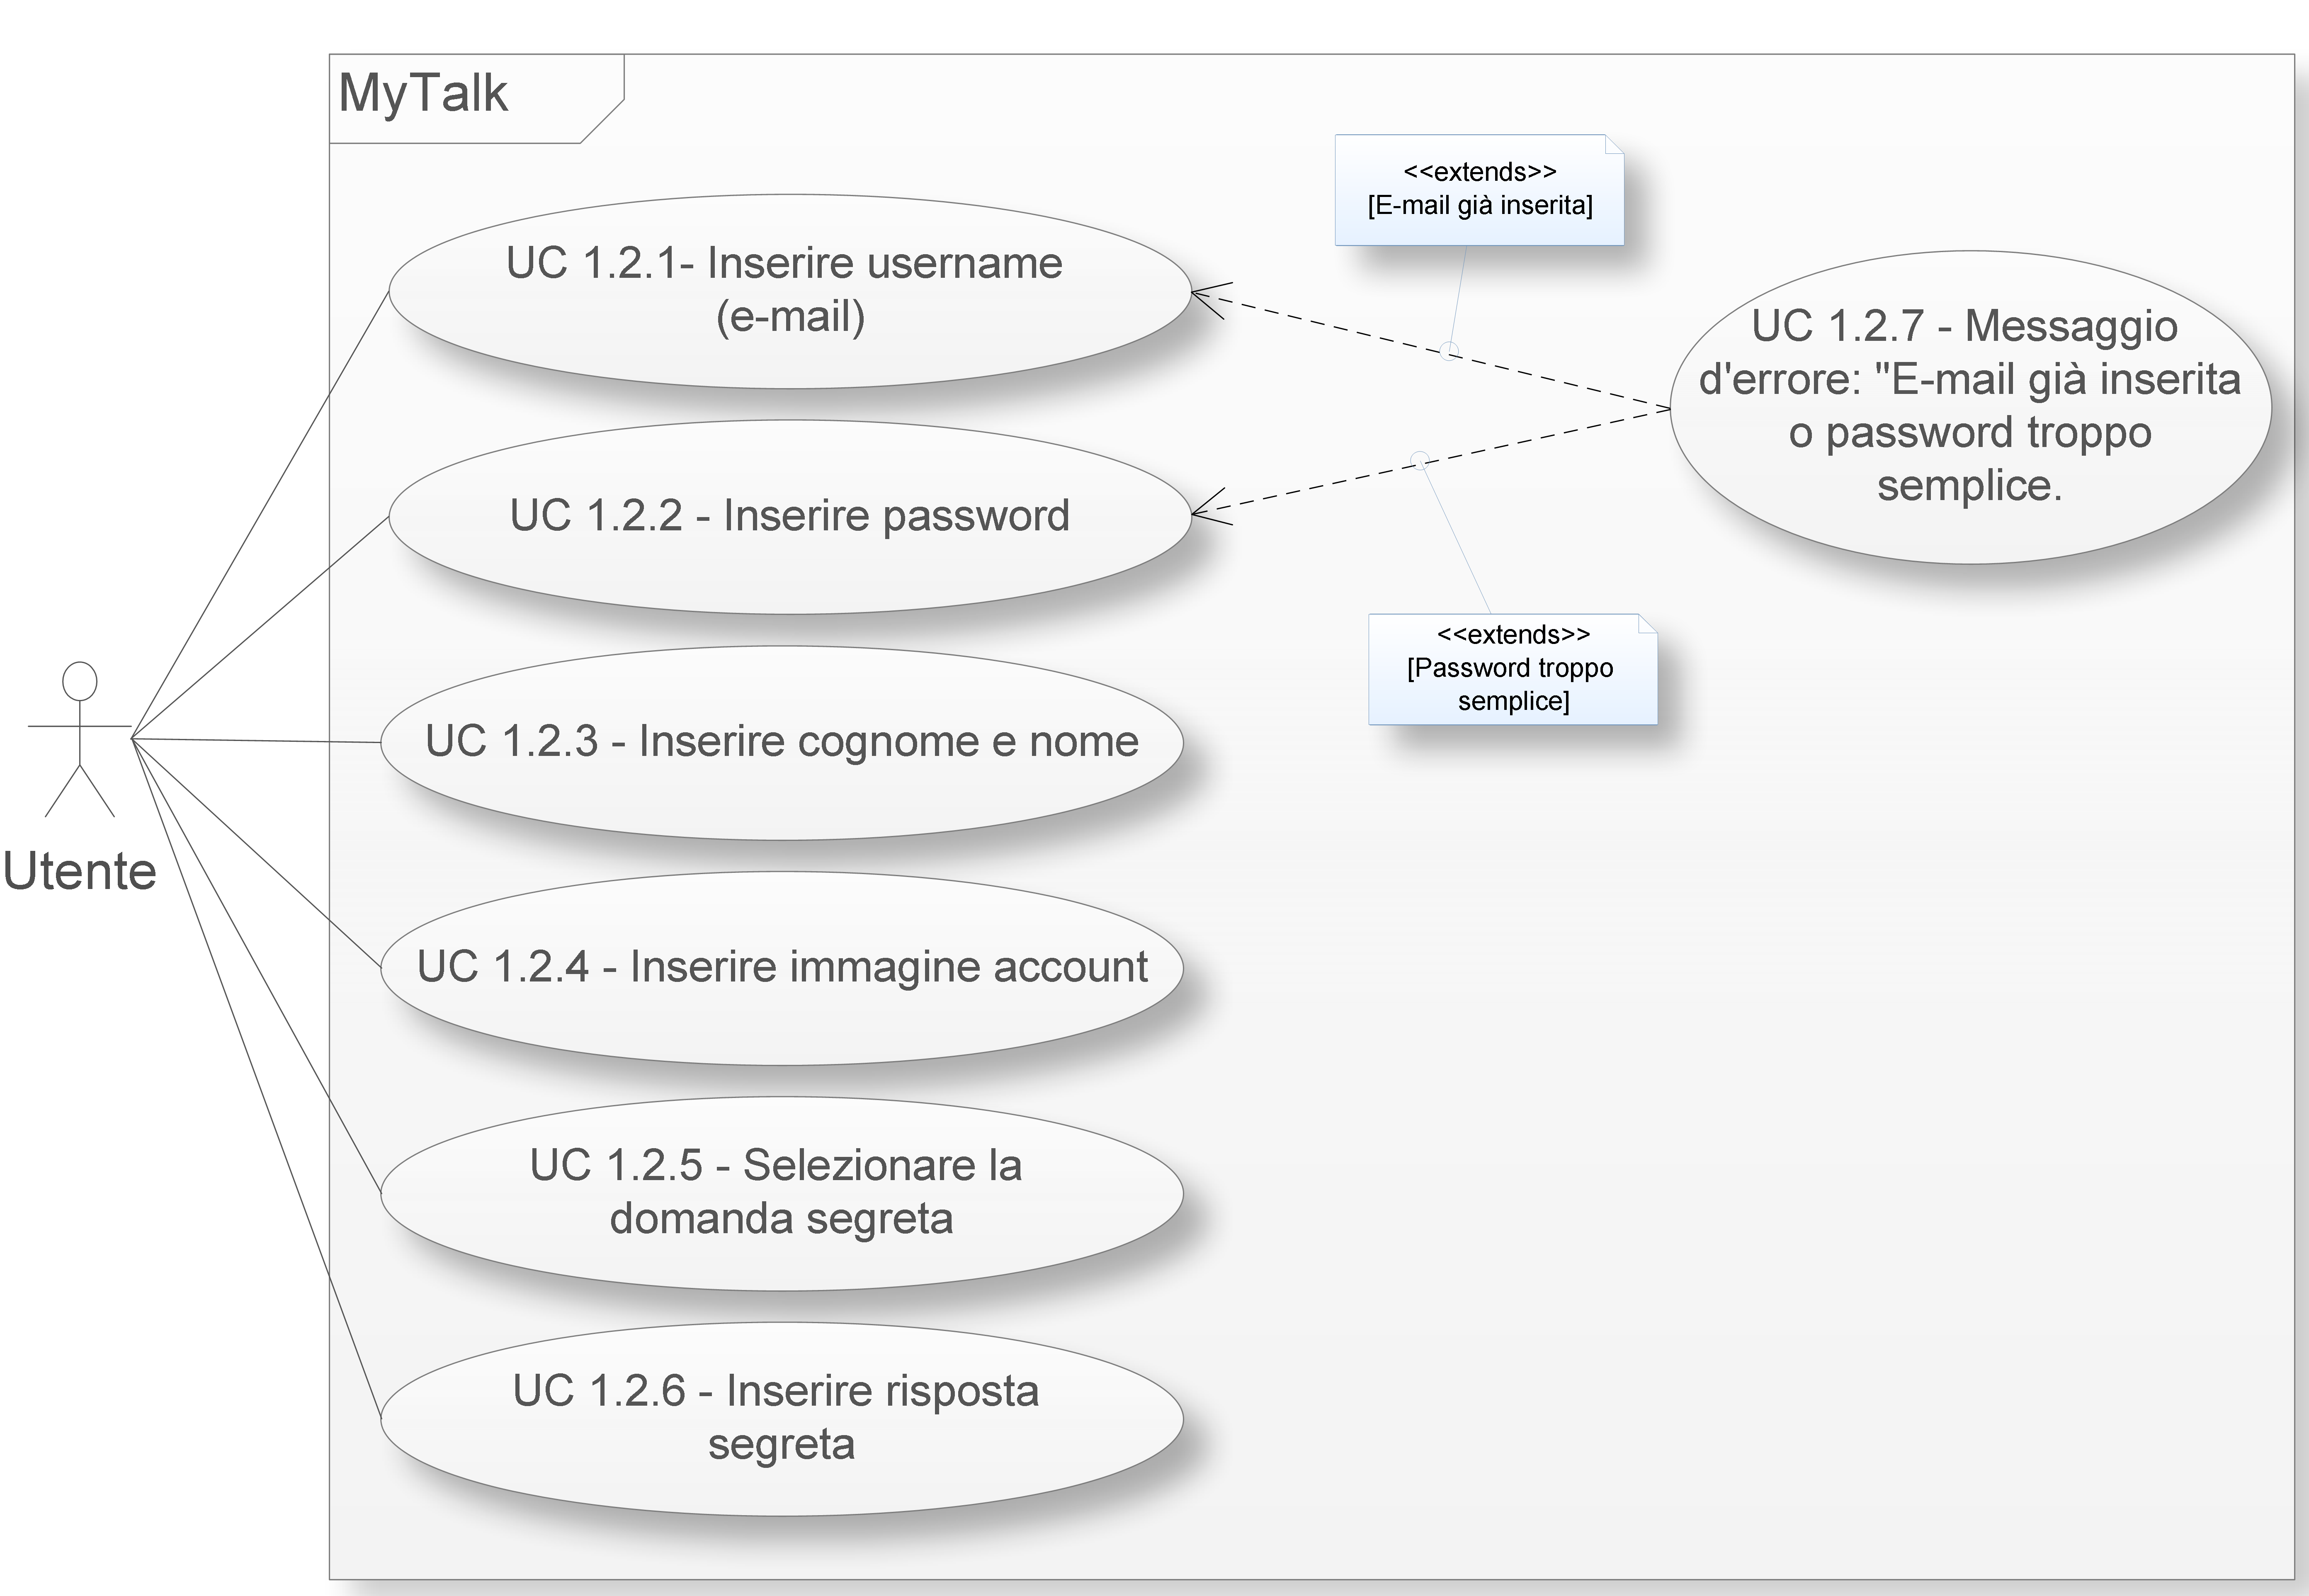
\includegraphics[width=.8\textwidth]{UC1-2}
\caption{}\label{fig:}
\end{center}
\end{figure}
\begin{description}
\item{\scshape\bfseries Attori principali:}Utente.
\item{\scshape\bfseries Scopo e descrizione:} L'utente si registra nel sistema.
\item{\scshape\bfseries Precondizione:} L'utente (generico) visualizza la schermata iniziale e il sistema è pronto.
\item{\scshape\bfseries Postcondizione:} L'utente si è registrato nel sistema MyTalk
\item{\scshape\bfseries Illustrazione scenario principale:} La registrazione di un nuovo account comporta l'inserimento di un indirizzo email come ID utente (UC1.2.1), una password (UC1.2.2), domanda segreta (UC1.2.6) e la relativa risposta (UC1.2.7). Il nome (UC1.2.3), il cognome (UC1.2.4) e un'immagine (UC1.2.5) da associare al proprio profilo possono essere inserite facoltativamente. Per andare a buon fine la procedura di registrazione richiede che la password prescelta assicuri un sufficiente livello di complessità e prevede altresì la selezione della domanda segreta (e della relativa risposta) necessarie al recupero della password in caso di smarrimento, nonché la validazione dell''indirizzo email al fine di verificare che l''utente ne sia effettivamente in possesso.
\item{\scshape\bfseries Illustrazione scenario alternativo:} Il sistema può fallire per via dell'inserimento di dati non corretti. Il sistema mostra un errore relativo all'username (UC1.2.8) oppure alla password (UC1.2.9)
\end{description}

\subsection{UC1.3: Recupero della password}
\begin{figure}[H]
\begin{center}
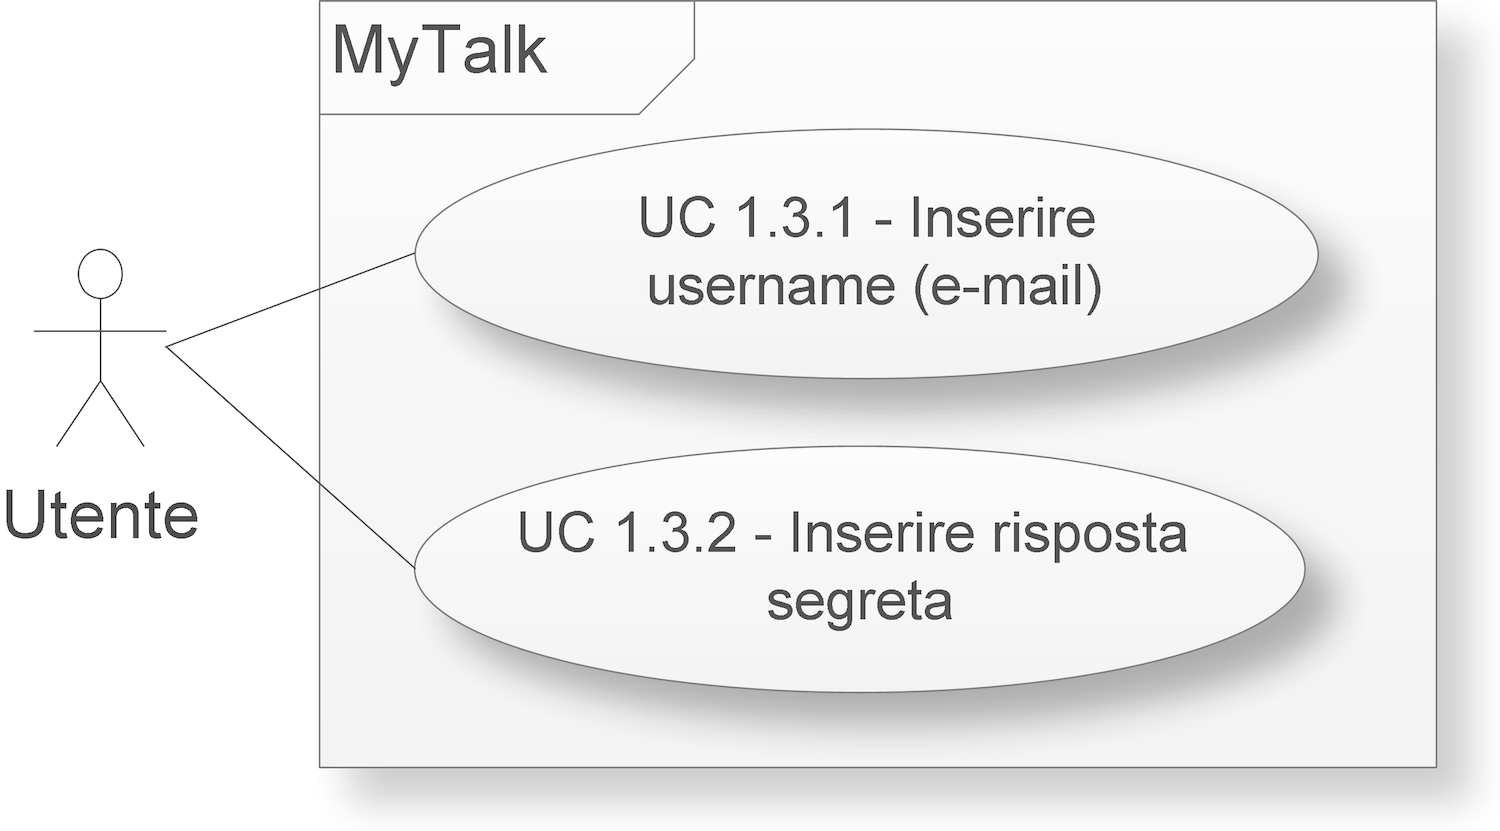
\includegraphics[width=.8\textwidth]{UC1-3}
\caption{}\label{fig:}
\end{center}
\end{figure}
\begin{description}
\item{\scshape\bfseries Attori principali:}Utente.
\item{\scshape\bfseries Scopo e descrizione:} L'utente desidera recuperare la password smarrita.
\item{\scshape\bfseries Precondizione:} L'utente (generico) visualizza la schermata iniziale e il sistema è pronto.
\item{\scshape\bfseries Postcondizione:} L'utente riceve per e-mail la password dimenticata.
\item{\scshape\bfseries Illustrazione scenario principale:} Si avvia la procedura di recupero della password: l'utente deve inserire l'e-mail (UC1.3.1) e la risposta alla domanda segreta (UC1.3.2). A questo segue l'invio della password all'indirizzo email indicato in fase di registrazione.
\item{\scshape\bfseries Illustrazione scenario alternativo:} Il sistema può fallire per via dell'inserimento di dati non corretti. Il sistema evidenzia gli errori e rimane in attesa della correzione.
\end{description}

\subsection{UC2: Home screen dell'applicativo}
\begin{figure}[H]
\begin{center}
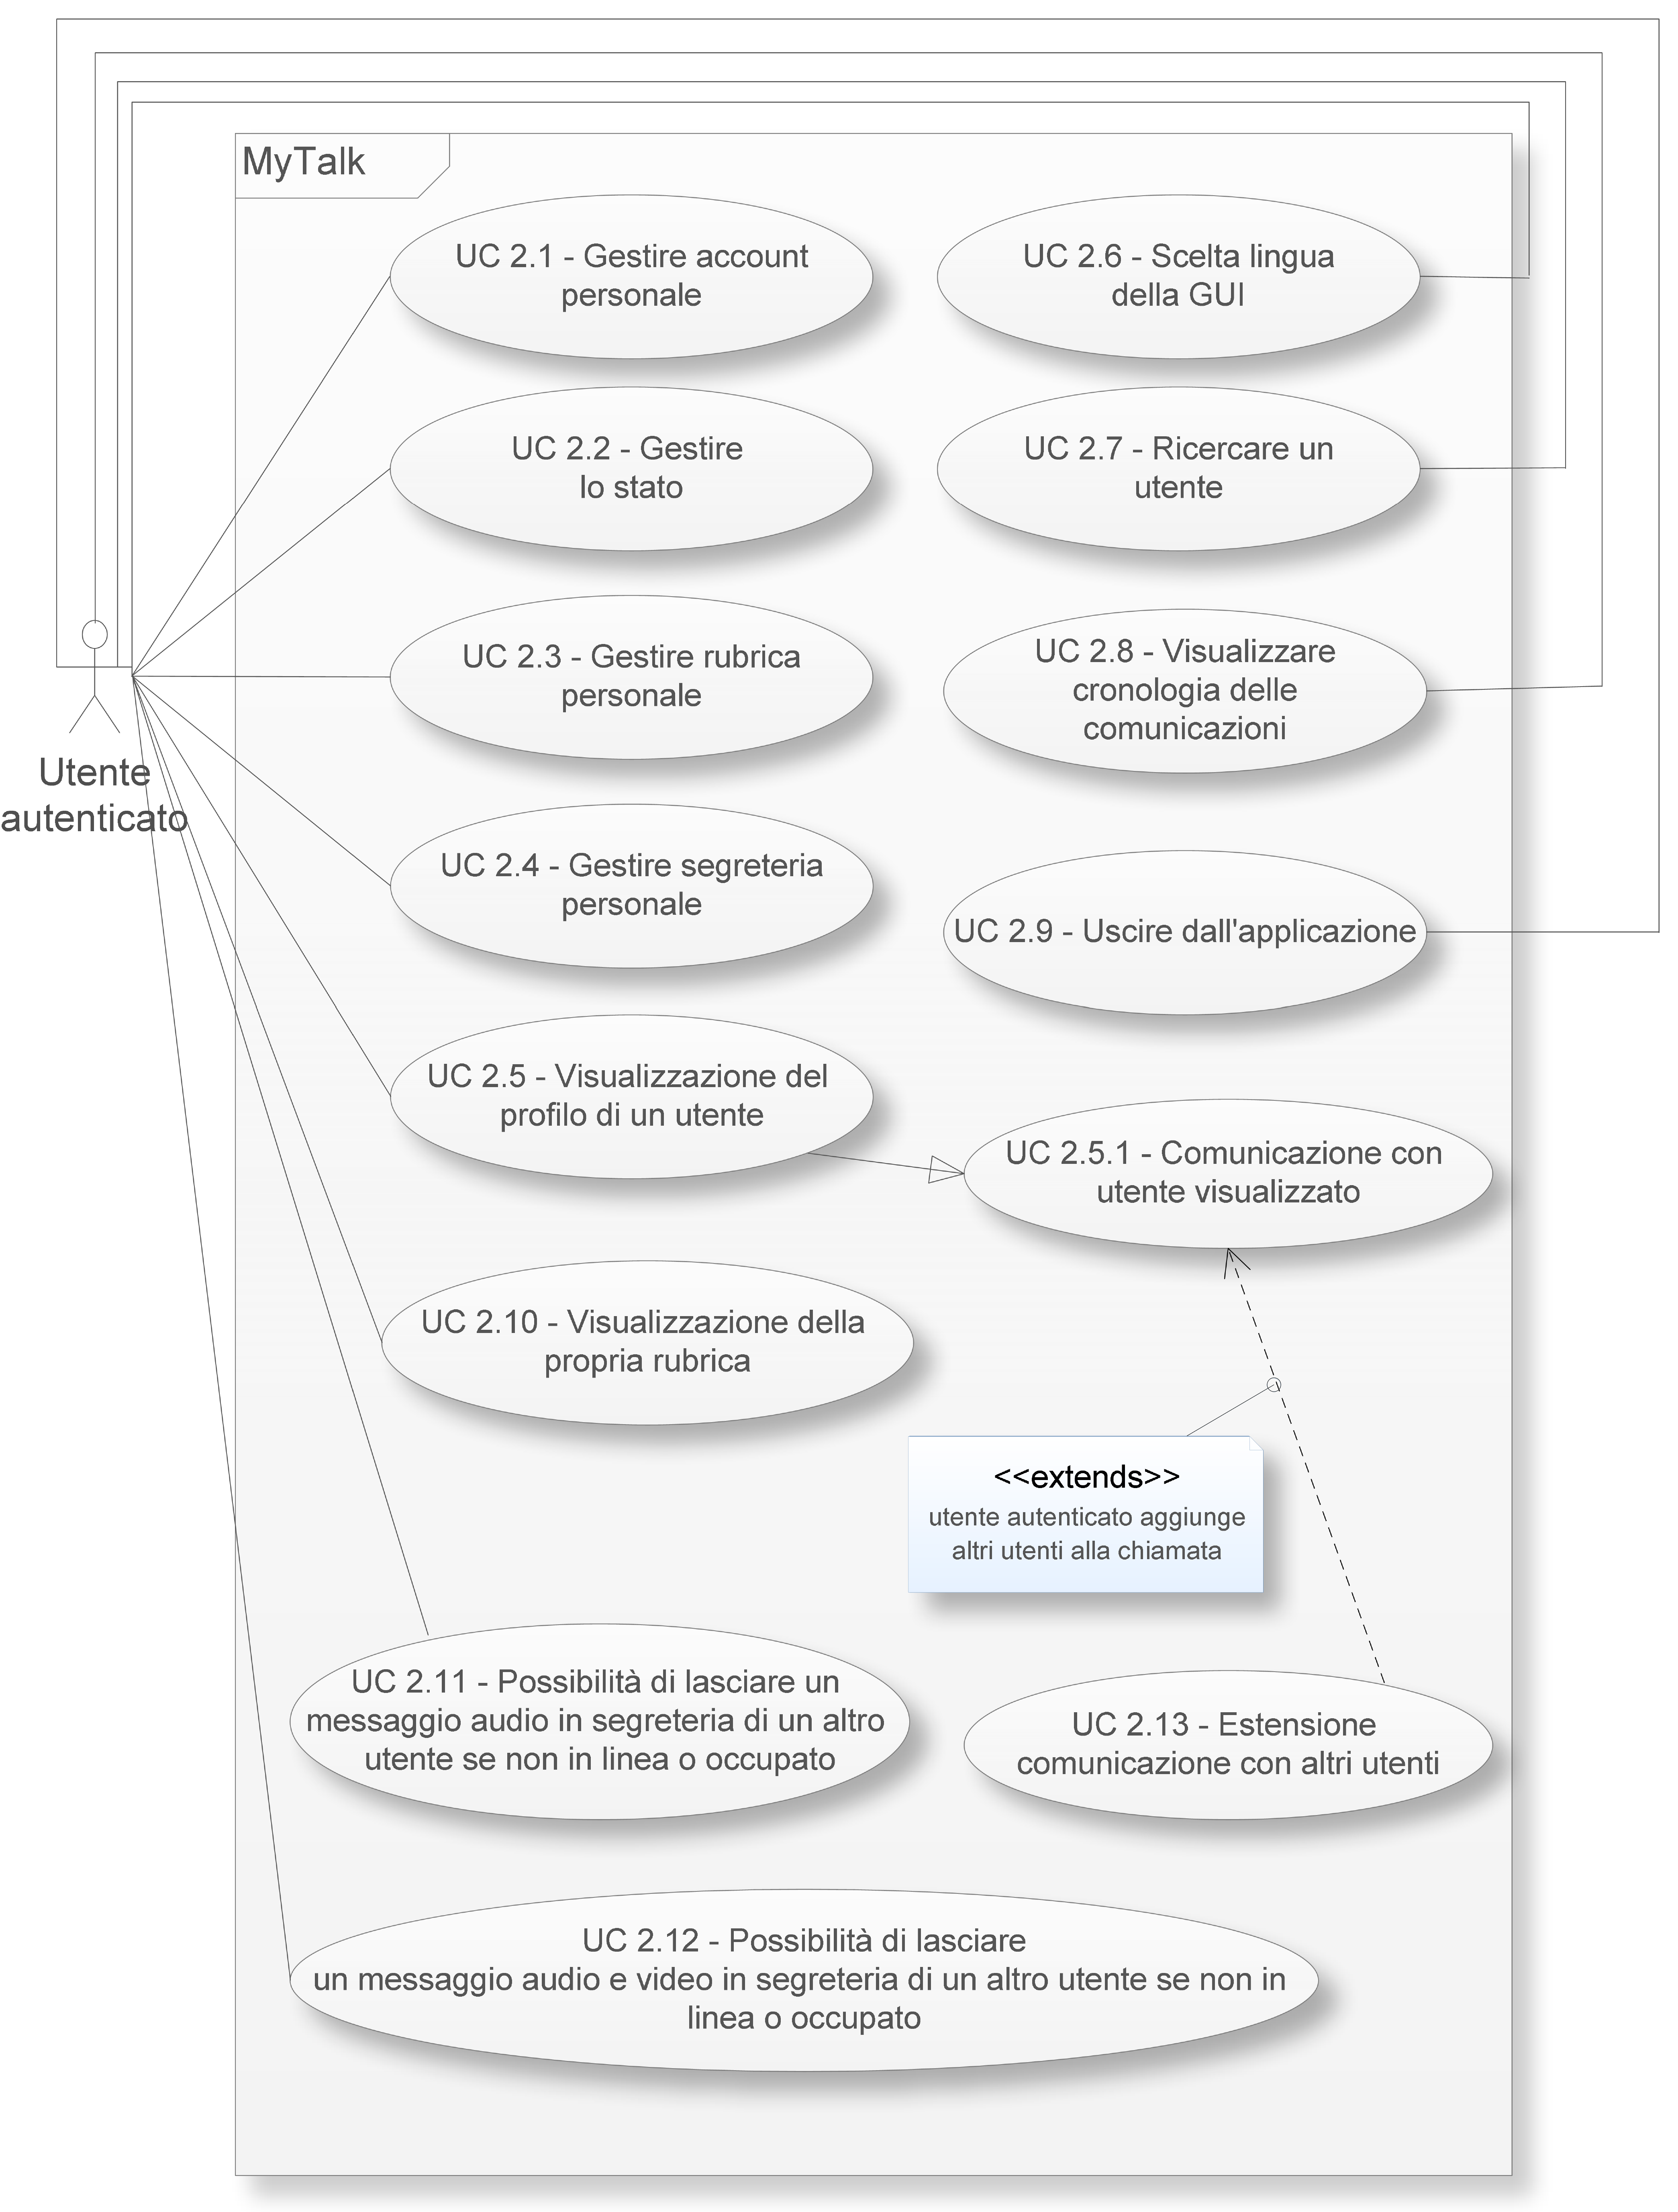
\includegraphics[width=.8\textwidth]{UC2}
\caption{}\label{fig:}
\end{center}
\end{figure}
\begin{description}
\item{\scshape\bfseries Attori principali:}Utente autenticato.
\item{\scshape\bfseries Scopo e descrizione:} Funzionalità generali offerte all'utente autenticato e presenti nella Home screen dell'applicativo.
\item{\scshape\bfseries Precondizione:} L'utente ha effettuato il login ed è autenticato nel sistema.
\item{\scshape\bfseries Postcondizione:} L'utente ha eseguito una delle funzioni proposte.
\item{\scshape\bfseries Illustrazione scenario principale:} L'utente dopo aver eseguito il login al sistema, si trova nella Home dell'applicativo. Qui può svolgere una delle seguenti operazioni: gestire il proprio account (UC2.1), scegliere la lingua della GUI (UC2.6), gestire lo stato (UC2.2), eseguire delle ricerche di utenti (UC2.7), gestire la propria rubrica (UC2.3), lasciare un messaggio nella segreteria di un utente se esso non è in linea o è occupato (UC2.11 - UC2.12), gestire la propria segreteria (UC2.4), visualizzare la cronologia delle comunicazioni (UC2.8), visualizzare la propria rubrica (UC2.10) e visualizzare il profilo di un utente (UC2.5) dopo averlo selezionato da una lista. Infine l'utente ha la possibilità di chiudere l'applicativo (UC2.9).
\item{\scshape\bfseries Illustrazione scenario alternativo:} L'utente, se ha già avviato una connessione con un altro utente, può estenderla con altri (UC2.12).
\end{description}

\subsection{UC2.1: Gestione account}
\begin{figure}[H]
\begin{center}
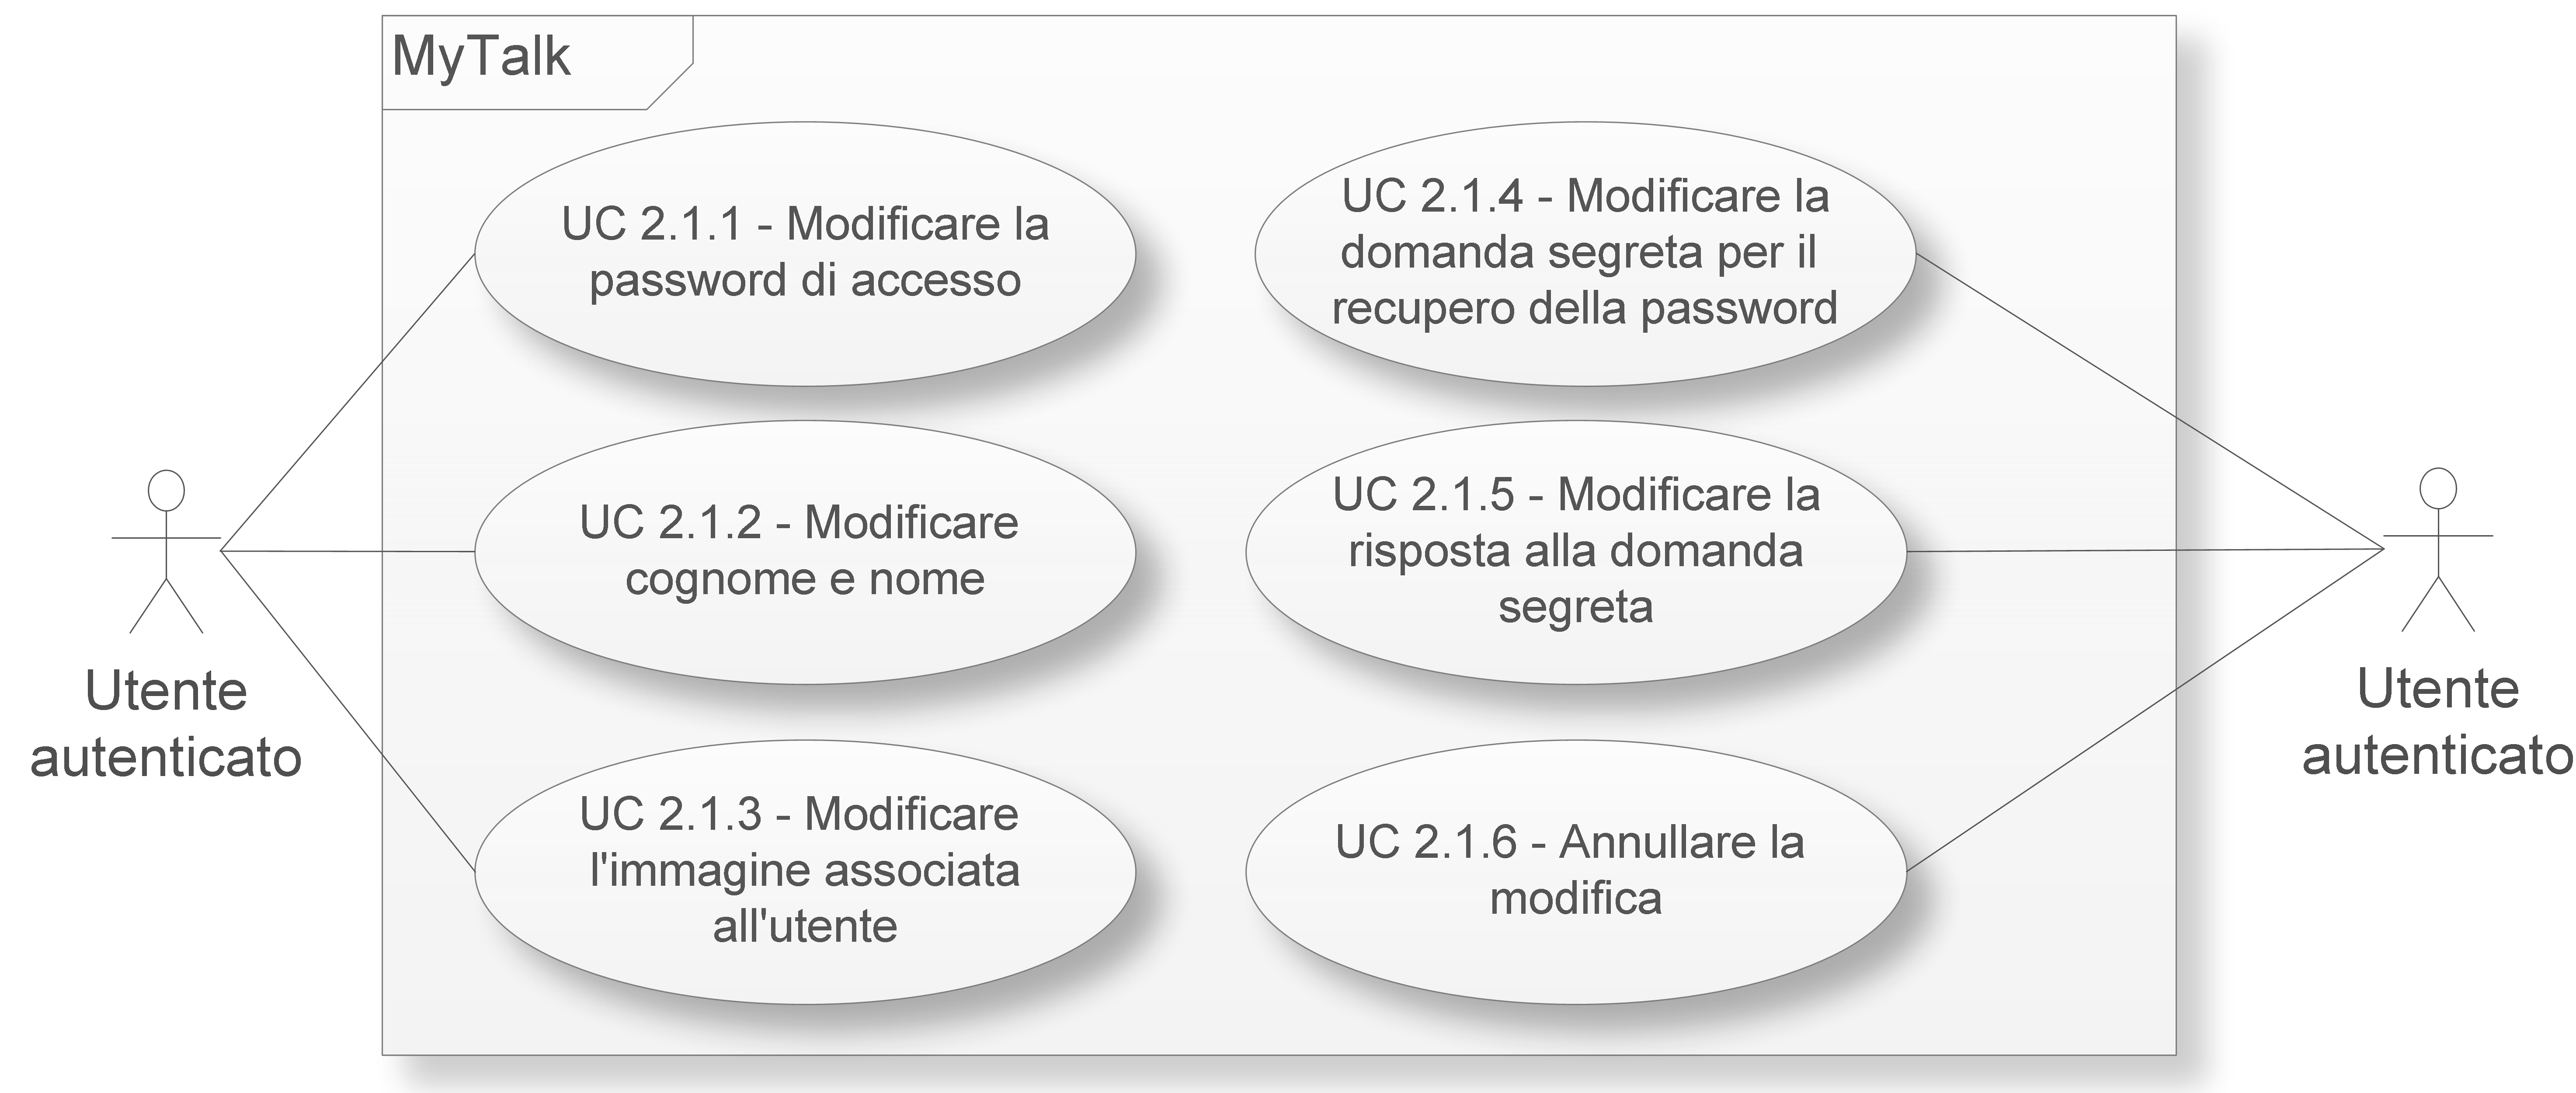
\includegraphics[width=.8\textwidth]{UC2-1}
\caption{}\label{fig:}
\end{center}
\end{figure}
\begin{description}
\item{\scshape\bfseries Attori principali:}Utente autenticato.
\item{\scshape\bfseries Scopo e descrizione:} un utente autenticato, ha la possibilità di modificare i propri dati personali, inseriti durante la sua registrazione, così da rimediare ad eventuali errori.
\item{\scshape\bfseries Precondizione:} l'utente corrente e' registrato nel sistema, ed ha effettuato il login.
\item{\scshape\bfseries Postcondizione:} i dati dell'utente sono stati aggiornati con i valori da lui inseriti.
\item{\scshape\bfseries Illustrazione scenario principale:} L'utente visualizza i valori correnti dei dati che lo riguardano e può apportare
le modifiche che ritiene necessarie. I dati che può modificare sono la password (UC2.1.1), il nome (UC2.1.2), il cognome (UC2.1.6), l'immagine profilo (UC2.1.3), la domanda segreta (UC2.1.4), la risposta alla domanda segreta (UC2.1.5). A questo punto può salvare le modifiche (UC2.1.8).
\item{\scshape\bfseries Illustrazione scenario alternativo:} Prima del salvataggio (UC2.1.8) l'utente può annullare l'operazione (UC2.1.7) tornando così alla schermata principale senza aver effettuato nessuna modifica.
\end{description}

\subsection{UC2.2: Gestire lo stato}
\begin{figure}[H]
\begin{center}
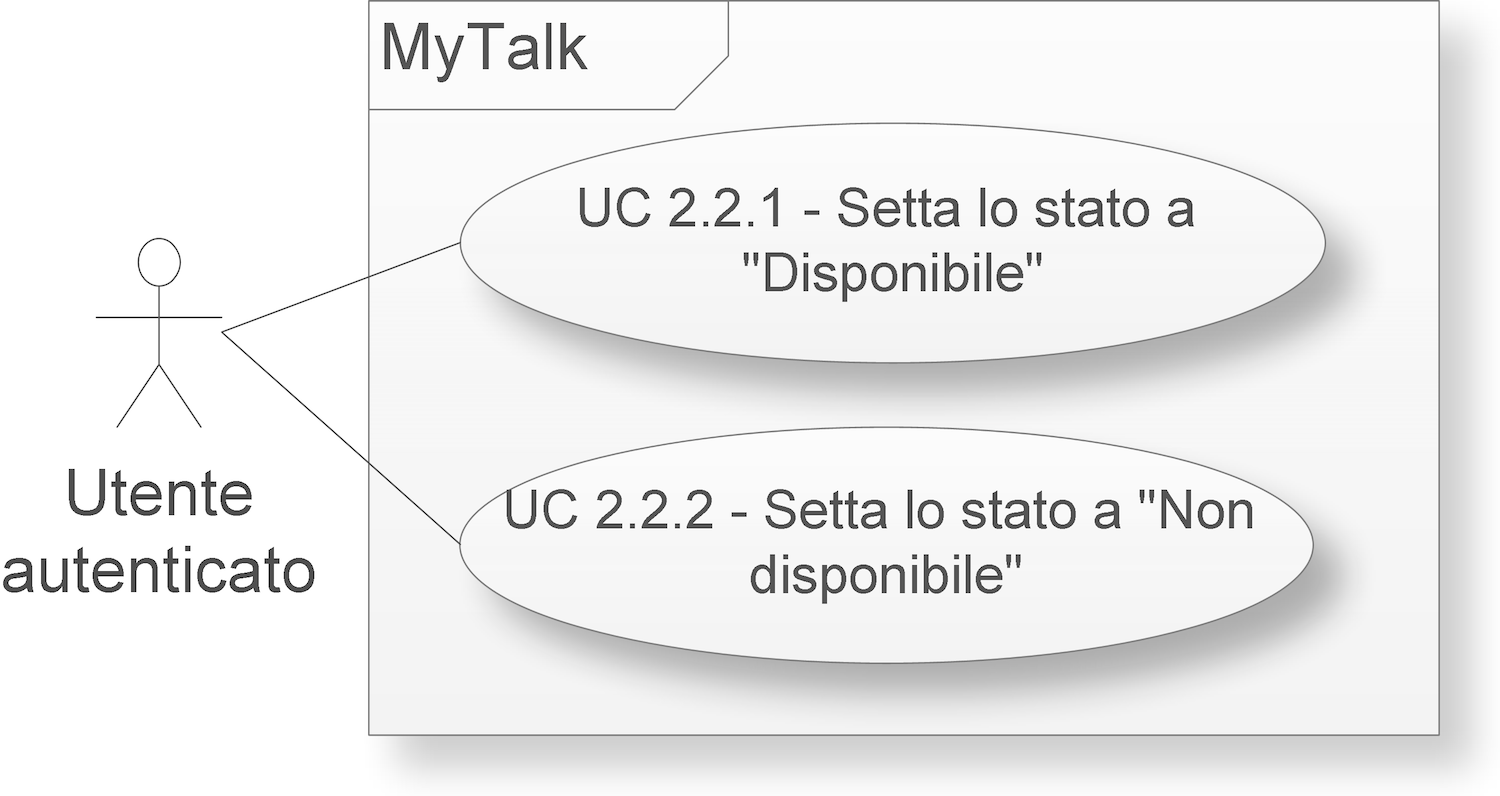
\includegraphics[width=.8\textwidth]{UC2-2}
\caption{}\label{fig:}
\end{center}
\end{figure}
\begin{description}
\item{\scshape\bfseries Attori principali:}Utente autenticato.
\item{\scshape\bfseries Scopo e descrizione:} L'utente potrà comunicare agli altri utenti la sua disponibilità o meno a comunicare, aggiornando il proprio stato.
\item{\scshape\bfseries Precondizione:} L'utente è registrato nel sistema ed ha eseguito l'accesso senza errori.
\item{\scshape\bfseries Postcondizione:} L'utente ha modificato il proprio stato.
\item{\scshape\bfseries Illustrazione scenario principale:} L'utente potrà scegliere di cambiare il proprio stato corrente. Gli stati tra cui può scegliere sono:disponibile (UC2.2.1)  e non disponibile (UC2.2.2).
\end{description}

\subsection{UC2.3: Gestione della rubrica}
\begin{figure}[H]
\begin{center}
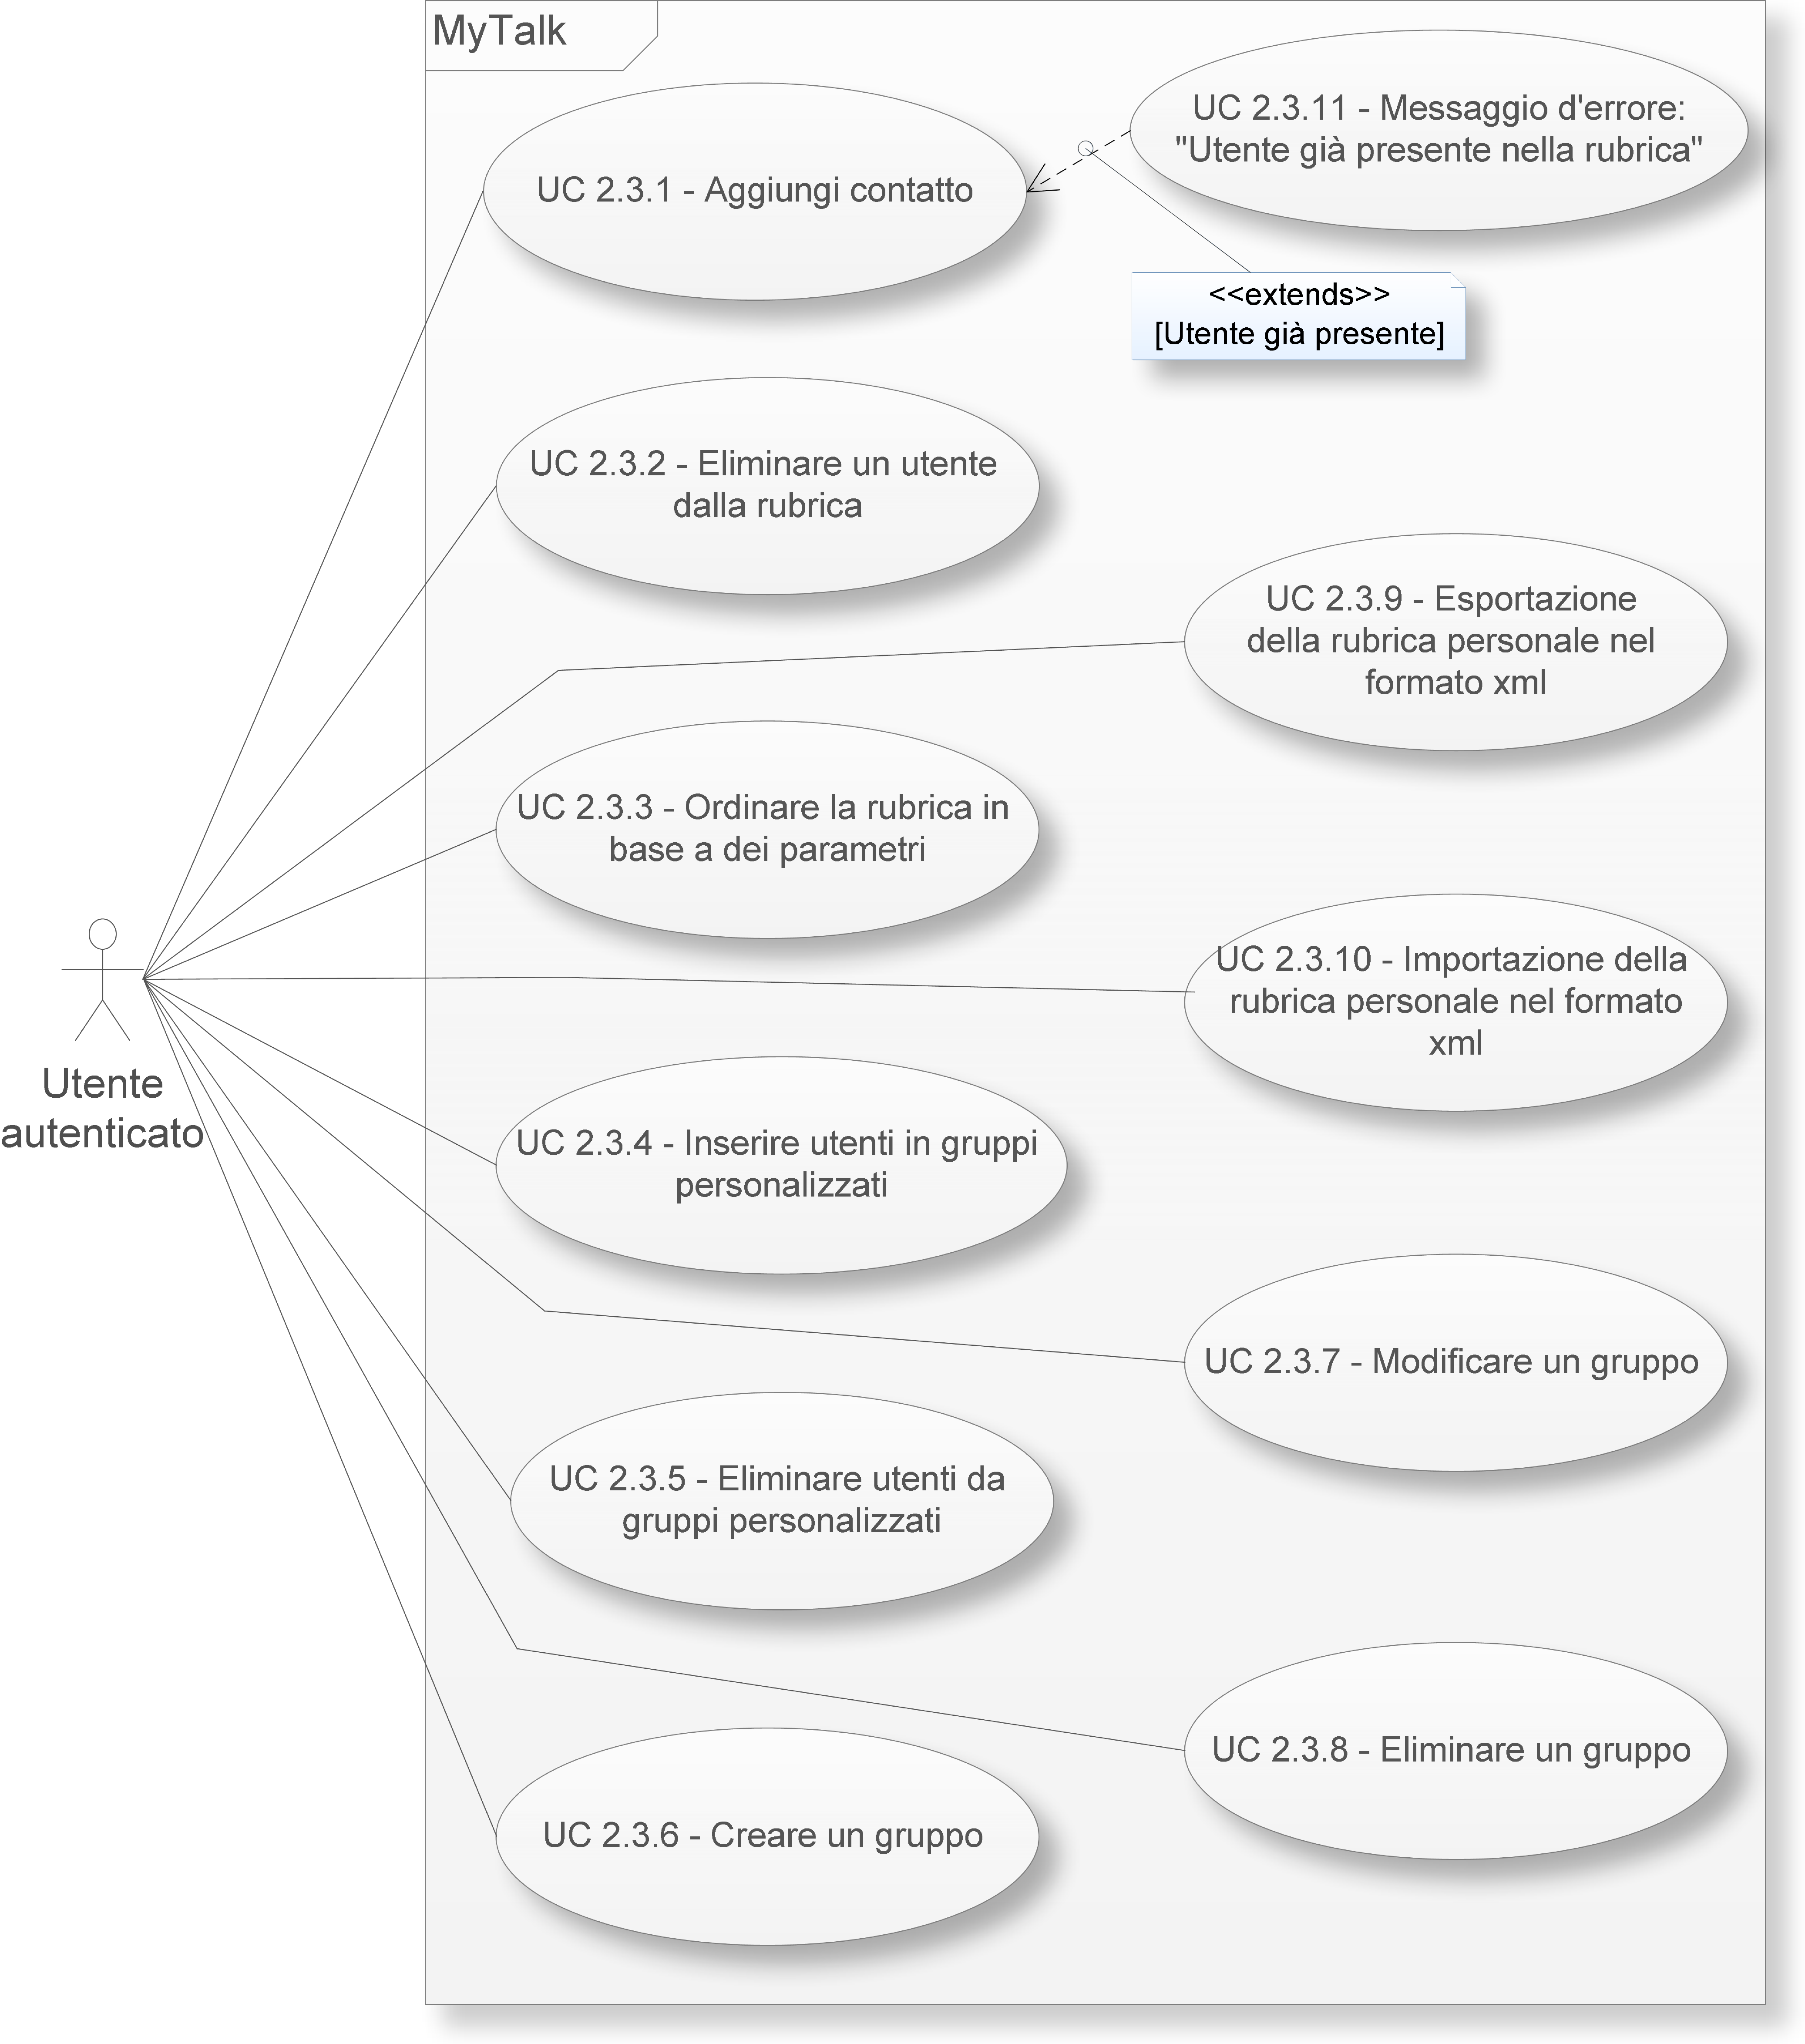
\includegraphics[width=.8\textwidth]{UC2-3}
\caption{}\label{fig:}
\end{center}
\end{figure}
\begin{description}
\item{\scshape\bfseries Attori principali:}Utente autenticato.
\item{\scshape\bfseries Scopo e descrizione:} L'utente può visualizzare ed organizzare la rubrica dei propri contatti personali sulla base della lista degli utenti che si sono registrati, oppure importando i contati da un file esterno.
\item{\scshape\bfseries Precondizione:} L'utente ha effettuato la procedura di login ed è quindi autenticato.
\item{\scshape\bfseries Postcondizione:} Se l'utente ha attuato delle modifiche, queste sono state salvate. Altrimenti non ci sono state modifiche sui dati inerenti la rubrica.
\item{\scshape\bfseries Illustrazione scenario principale:} L'utente visualizza la propria rubrica divisa in gruppi. Può quindi scegliere una delle seguenti opzioni: aggiunge un contatto alla rubrica tramite ricerca (UC2.3.1), aggiunge un contatto in gruppi personalizzati (UC2.3.4), crea un nuovo gruppo (UC2.3.6); elimina un gruppo (UC2.3.8), aggiunge ed eliminare un contatto alla rubrica in un gruppo scelto tra quelli già creati (UC2.3.4 - UC2.3.5), elimina un contatto dalla propria rubrica (UC2.3.2), esporta i contatti presenti nella propria rubrica (UC2.3.9) e importa dei contatti prelevati da un file XML (UC2.3.10).
Inoltre potrà ordinare la rubrica in base a dei parametri (UC2.3.3).
\item{\scshape\bfseries Illustrazione scenario alternativo:} Se la ricerca del contatto da esito negativo viene riportato un errore (UC2.3.1.3).
\item{\scshape\bfseries Illustrazione scenario alternativo:} Se il contatto selezionato per l'inserimento nella rubrica, è già presente nella rubrica, allora compare un messaggio d'errore (UC2.3.1.3) che avvisa l'utente dell'impossibilità di aggiungere il contatto. (Non vengono visualizzati due errori separati ma un errore unico).
\end{description}

\subsection{UC2.4: Gestire segreteria personale}
\begin{figure}[H]
\begin{center}
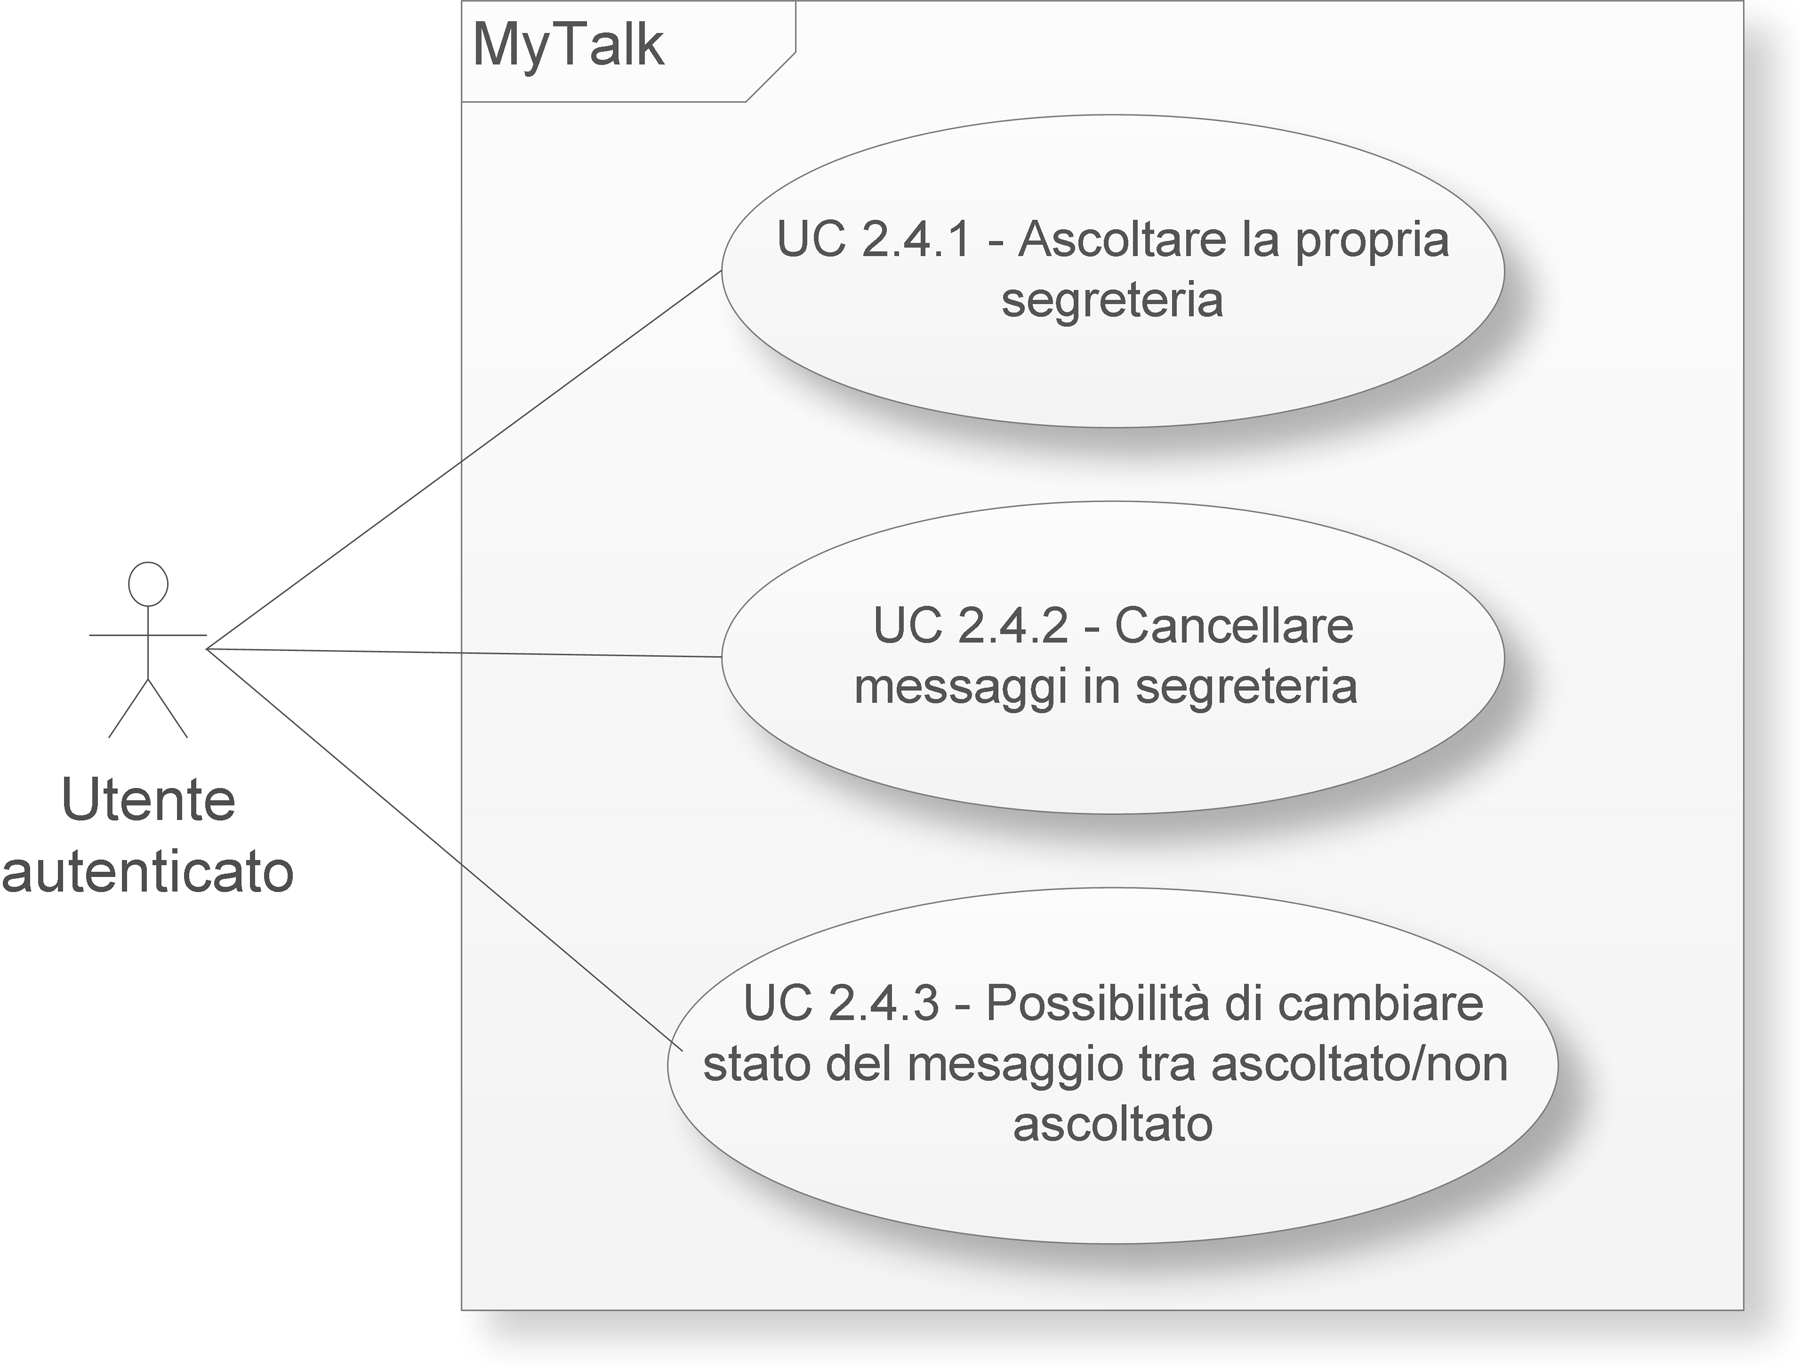
\includegraphics[width=.8\textwidth]{UC2-4}
\caption{}\label{fig:}
\end{center}
\end{figure}
\begin{description}
\item{\scshape\bfseries Attori principali:}Utente autenticato.
\item{\scshape\bfseries Scopo e descrizione:} L'utente ha a disposizione una segreteria personale che può gestire.
\item{\scshape\bfseries Precondizione:} L'utente ha effettuato la procedura di login ed è quindi autenticato.
\item{\scshape\bfseries Postcondizione:} Il sistema ha eseguito con successo le operazioni richieste dall'utente.
\item{\scshape\bfseries Illustrazione scenario principale:} L'utente si trova nella sezione riguardante la segreteria e può ascoltare, se presenti, i messaggi lasciati dai propri contatti (UC2.4.1), cancellarle i messaggi ricevuti (UC2.4.2) ed infine cambiare lo stato del messaggio da letto a da leggere e viceversa.
\end{description}

\subsection{UC2.5.1: Connessione con altri utenti autenticati}
\begin{figure}[H]
\begin{center}
\includegraphics[width=.8\textwidth]{UC2-5-1}
\caption{}\label{fig:}
\end{center}
\end{figure}
\begin{description}
\item{\scshape\bfseries Attori principali:}Utente autenticato.
\item{\scshape\bfseries Scopo e descrizione:} Un utente, durante una chiamata audio, audio/video e chat, può eseguire diverse operazioni sulla connessione stabilita.
\item{\scshape\bfseries Precondizione:} L'utente è autenticato nel sistema, ed ha già stabilito una connessione con un utente autenticato.
\item{\scshape\bfseries Postcondizione:} L'utente ha concluso la comunicazione. La causa della terminazione può essere attribuita alla chiusura volontaria della connessione oppure al fatto che l'utente rimane l'unico attivo nella connessione.
\item{\scshape\bfseries Illustrazione scenario principale:} L'utente ha avviato una comunicazione. Mentre questa è in esecuzione, l'utente potrà: visualizzare le statistiche sulla comunicazione (UC2.5.1.1), condividere delle risorse dal proprio dispositivo (Condivisione di PDF, invio di file, condivisione di una lavagna grafica, e condivisione dello schermo)(UC2.5.1.2), visualizzare da quanto tempo è aperta la connessione (UC2.5.1.3), avviare e fermare una registrazione (UC2.5.1.6 - UC2.5.1.7), accettare o rifiutare una richiesta di registrazione inoltrata da un interlocutore (UC2.5.1.4 - UC2.5.1.5). Infine l'utente può decidere di terminare la comunicazione (UC2.5.1.8).
\end{description}

\subsection{UC2.5.1.1: Visualizzazione statistiche sulla comunicazione}
\begin{figure}[H]
\begin{center}
\includegraphics[width=.8\textwidth]{UC2-5-1-1}
\caption{}\label{fig:}
\end{center}
\end{figure}
\begin{description}
\item{\scshape\bfseries Attori principali:}Utente autenticato.
\item{\scshape\bfseries Scopo e descrizione:} L'utente visualizza i dettagli della comunicazione con un altro utente.
\item{\scshape\bfseries Precondizione:} L'utente sta comunicando con un altro utente del sistema.
\item{\scshape\bfseries Postcondizione:} L'utente ha visualizzato tutte le informazioni riguardanti la comunicazione.
\item{\scshape\bfseries Illustrazione scenario principale:} L'utente che comincia a comunicare con un altro utente ha a disposizione la visualizzazione di alcune informazioni sulla comunicazione in corso, come il numero di byte ricevuti ed inviati (UC2.5.1.1.1 - UC2.5.1.1.3), la latenza ossia il tempo che passa da quando un utente trasmette a quando l'altro utente riceve (UC2.5.1.1.5), la velocità di trasmissione dei dati (UC2.5.1.1.2) e i frame per secondo (fps) nel caso sia in corso una videochiamata (UC2.5.1.1.4).
\end{description}

\subsection{UC2.7: Ricerca di un utente}
\begin{figure}[H]
\begin{center}
\includegraphics[width=.8\textwidth]{UC2-7}
\caption{}\label{fig:}
\end{center}
\end{figure}
\begin{description}
\item{\scshape\bfseries Attori principali:}Utente autenticato.
\item{\scshape\bfseries Scopo e descrizione:} L'utente desidera ricercare altri utenti all'interno del sistema.
\item{\scshape\bfseries Precondizione:} L'utente è autenticato al sistema; la lista degli utenti registrati presso il server non è vuota.
\item{\scshape\bfseries Postcondizione:} L'utente ha ottenuto una lista (possibilmente vuota) di utenti che soddisfano i parametri di ricerca.
\item{\scshape\bfseries Illustrazione scenario principale:} Nel momento in cui un utente vuole ricercare un altro utente registrato nel sistema, ha la possibilità  di ricercarlo o nella propria rubrica (UC2.7.1) o nella lista di utenti registrati nel sistema (UC2.7.2).
\end{description}

\newpage\section{Requisiti di prodotto}
I requisiti verranno suddivisi in base alla loro priorità. Rispettivamente seguirà la lista dei requisiti obbligatori, facoltativi e desiferabili. Ogni requisito è identificato con il seguente formato RXYZI con:


		\begin{itemize}

			\item \textbf{X}: indica la tipologia dell'utente interessato dal requisito. I possibili valori che X può assumere sono U (utente) oppure S (sistema).

			\item \textbf{Y}: indica la tipologia del requisito, e può assumere i valori: F(funzionale), Q(qualitativo), P(prestazionale), D(dichiarativo).

			\item \textbf{Z}: indica il livello di priorità del requisito. Può assumere i valori O(obbligatorio), \\F(facoltativo), D(desiderabile).

			\item \textbf{I}: indica l'id numerico del requisito, denominato secondo le direttive delle norme di progetto.

		\end{itemize}


		Ogni requisito si può suddividere in sottorequisiti. Tale evento è evidenziato dal valore del campo I, come riportato nelle norme di progetto. Infine i requisiti sono ordinati (nelle proprie sezioni) in base all'ordine crescente del campo numerico I.\
Per quanto riguarda invece i requisiti di processo, si rimanda ai documenti \textit{piano\_di\_qualifica.2.0.pdf} (sez. 3.1) e \textit{norme\_di\_progetto.2.0.pdf} (in particolare le sez. 2, 3 e 4).

\subsection{Requisiti funzionali}


\subsubsection{Requisiti funzionali obbligatori}

\begin{center}
\rowcolors{2}{lightblue}{llightblue}\begin{longtable}{lp{.55\textwidth}l}
\toprule Codice & Requisito & Fonte\\
\midrule
RUFO1.0.0 & L'utente deve potersi autentificare nel server, così da permettere a quest'ultimo di rilevare la sua presenza nel sistema. & Interno \\
RSFO1.2.0 & Per effettuare il login è necessario inserire i dati utente & Interno\\
RSFO1.2.1 & Per effettuare il login è necessario inserire il proprio username & Interno\\
RSFO1.2.2 & Per effettuare il login è necessario inserire la propria password & Interno\\
RUFO2.0.0 & Registrazione del nuovo utente & Capitolato d'appalto \\
RSFO2.1.0 & Inserimento dei dati obbligatori per l’autenticazione & Interno \\
RSFO2.1.3 & Inserimento del campo obbligatorio username (e-mail) & Interno\\
RSFO2.1.4 & Inserimento del campo obbligatorio password & Interno\\
RSFO2.1.5 & Inserimento del campo obbligatorio ``domanda segreta'' & Interno\\
RSFO2.1.6 & Inserimento del campo obbligatorio ``risposta alla domanda segreta'' & Interno\\
RUFO5.0.0 & Possibilità di visualizzare la lista di utenti registrati nel sistema & Capitolato d'appalto \\
RUFO6.1.0 & stabilire una comunicazione audio con un utente in linea & Capitolato d'appalto \\
RUFO6.1.1 & Stabilire una comunicazione audio mediante inserimento d'indirizzo IP & Capitolato d'appalto \\
RUFO6.1.3 & Stabilire una comunicazione audio con un utente registrato e NON presente nella rubrica & Capitolato d'appalto \\
RUFO6.2.0 & Stabilire una comunicazione audio e video con un utente in linea & Capitolato d'appalto \\
RUFO6.2.1 & Stabilire una comunicazione audio e video mediante inserimento d'indirizzo IP & Capitolato d'appalto \\
RUFO6.2.3 & Stabilire una comunicazione audio e video con un utente registrato e NON presente nella rubrica & Capitolato d'appalto \\
RUFO6.4.0 & Mantenere la comunicazione audio e video fino a che uno dei due utenti non la chiude & Capitolato d'appalto \\
RUFO6.5.0 & Mantenere la comunicazione audio fino a che uno dei due utenti non la chiude & Capitolato d'appalto \\
RUFO7.0.0 & Indicare il tempo di comunicazione & Capitolato d'appalto \\
RUFO8.0.0 & Valutare il numero di byte trasmessi & Capitolato d'appalto \\
RUFO8.1.0 & Valutare il numero di byte inviati & Interno \\
RUFO8.2.0 & Valutare il numero di byte ricevuti & Interno \\
RUFO9.0.0 & Indicare la qualità della linea di trasmissione & Capitolato d'appalto \\
RUFO9.1.0 & Rilevare latenza & Capitolato d'appalto \\
RUFO9.2.0 & Rilevare velocità di trasmissione & Capitolato d'appalto \\
RSFO11.0.0 & Creare una connessione tra client, mediante l'utilizzo di un server & Capitolato d'appalto \\
RSFO11.1.0 & Utilizzo del protocollo webSocket per creare una connessione tra 2 utenti & Interno \\
RSFO12.0.0 & Gestire gli eventi dell'utente durante la connessione. & Interno \\
RUFO12.3.0 & Chi partecipa alla connessione può togliersi da essa & Interno \\
\bottomrule
\end{longtable}
\end{center}

\subsubsection{Requisiti funzionali desiderabili}

\begin{center}
\rowcolors{2}{lightblue}{llightblue}\begin{longtable}{lp{.55\textwidth}l}
\toprule Codice & Requisito & Fonte\\
\midrule
RUFD1.1.0 & Gestione password dimenticata & Interno \\
RUFD1.1.1 & Proporre la domanda segreta all'utente & Interno \\
RUFD1.1.2 & Invio di una mail all'utente contenete la password dimenticata & Interno \\
RSFD2.1.2 & Convalidare username (e-mail) dell'utente & Interno \\
RUFD12.2.0 & Chi crea la connessione può eliminare i membri del gruppo di chiamata & Interno \\
RUFD13.1.0 & Servizio chat tra 2 utenti & Interno \\
RSFD21.0.0 & Gestione interfaccia grafica in più lingue & Interno \\
\bottomrule
\end{longtable}
\end{center}

\subsubsection{Requisiti funzionali facoltativi}

\begin{center}
\rowcolors{2}{lightblue}{llightblue}\begin{longtable}{lp{.55\textwidth}l}
\toprule Codice & Requisito & Fonte\\
\midrule
RUFF3.0.0 & Modifica dati utente & Interno \\
RUFF3.1.0 & Modifica dei dati per l'autenticazione & Interno \\
RUFF3.1.1 & Modifica della password & Interno\\
RUFF3.1.2 & Modifica della ``domanda segreta'' & Interno\\
RUFF3.1.3 & Modifica della ``risposta alla domanda segreta'' & Interno\\
RUFF3.2.0 & Modifica dei dati anagrafici facoltativi & Interno \\
RUFF3.2.1 & Modifica del nome & Interno\\
RUFF3.2.2 & Modifica del cognome & Interno\\
RUFF3.2.3 & Modifica dell'immagine profilo & Interno\\
RUFF4.0.0 & L'utente ha a disposizione una rubrica personale & Interno \\
RUFF4.1.0 & Possibilità d'inserire utenti nella propria rubrica & Capitolato d'appalto \\
RUFF4.2.0 & Possibilità di eliminare un utente dalla propria rubrica & Interno \\
RUFF4.3.0 & Possibilità di ordinare la rubrica su alcuni parametri rilevanti & Interno \\
RUFF4.3.1 & Possibilità di ordinare la rubrica in relazione al nome utente & Interno\\
RUFF4.3.2 & Possibilità di ordinare la rubrica in relazione al nome dei gruppi & Interno\\
RUFF4.4.0 & Possibilità di suddividere la rubrica in gruppi & Interno \\
RUFF4.4.1 & Possibilità di togliere un elemento da un gruppo & Interno \\
RUFF4.4.2 & Possibilità di aggiungere un elemento in un gruppo & Interno \\
RUFF4.4.3 & Possibilità di creare un gruppo & Interno \\
RUFF4.4.4 & Possibilità di eliminare un gruppo & Interno \\
RUFF4.5.0 & Possibilità di esportare in xml la rubrica personale & Interno \\
RUFF4.6.0 & Possibilità di modificare la rubrica importando un file xml & Interno \\
RUFF4.7.0 & Ricerca di un utente nella propria rubrica. & Interno \\
RUFF4.7.1 & Ricerca degli utenti nel cui nome compare la parola ricercata & Interno\\
RUFF4.7.2 & Ricerca degli utenti nel cui cognome compare la parola ricercata & Interno\\
RUFF4.7.3 & Ricerca degli utenti appartenenti ad un gruppo nel cui nome compare la parola ricercata & Interno\\
RUFF5.1.0 & Possibilità di cercare un utente dalla lista & Interno \\
RUFF5.1.1 & Possibilità di cercare un utente dalla lista, in relazione al nome utente & Interno\\
RUFF5.1.2 & Possibilità di cercare un utente dalla lista, in relazione al email & Interno\\
RUFF6.1.2 & Stabilire una comunicazione audio con un utente registrato e presente nella rubrica & Capitolato d'appalto \\
RUFF6.1.4 & Promuovere una comunicazione audio avviata con un utente in una comunicazione audio e video & Interno \\
RUFF6.2.2 & Stabilire una comunicazione audio e video con un utente presente nella rubrica & Capitolato d'appalto \\
RUFF6.2.4 & Declassare una comunicazione audio e video avviata con un utente in una comunicazione solo audio & Interno \\
RUFF6.2.5 & Disattivare la webcam utente pur continuando a ricevere il segnale video proveniente dall'altro capo della comunicazione & Interno \\
RUFF6.3.0 & Disattivare il microfono utente pur continuando a ricevere il segnale video proveniente dall'altro capo della comunicazione & Interno \\
RUFF9.3.0 & Rilevazione frame per secondo & Interno \\
RSFF11.2.0 & Utilizzo del protocollo webSocket per creare una connessione tra più di 2 utenti & Interno \\
RSFF12.1.0 & Estendere la connessione ad altri client & Interno \\
RUFF13.0.0 & Servizio chat testuale & Capitolato d'appalto \\
RUFF13.2.0 & Servizio chat tra più di 2 utenti & Interno \\
RUFF14.0.0 & Registrazione della chiamata & Capitolato d'appalto \\
RUFF14.1.0 & Necessità di autorizzazione dagli utenti della chiamata per poter avviare la registrazione & Interno \\
RUFF14.2.0 & Registrazione audio & Interno \\
RUFF14.3.0 & Possibilità di riascoltare la registrazione & Interno \\
RUFF15.0.0 & L'utente avrà a disposizione una segreteria telefonica. & Interno \\
RUFF15.1.0 & Possibilità di lasciare un audio messaggio in segreteria & Interno \\
RUFF15.2.0 & Possibilità di lasciare un audio e video messaggio in segreteria & Capitolato d'appalto \\
RUFF15.3.0 & Possibilità di ascoltare la propria segreteria & Interno \\
RUFF15.4.0 & Possibilità di cancellare messaggi della segretaria & Interno \\
RUFF15.5.0 & Possibilità di cambiare lo stato del messaggio da "non ascoltato" a "ascoltato" & Interno \\
RUFF16.0.0 & Fornire la possibilità di cambiare lo stato utente & Interno \\
RUFF16.1.0  & Fornire la possibilità di impostare 'disponibile' come stato utente & Interno \\
RUFF16.2.0 & Fornire la possibilità di impostare 'non disponibile' come stato utente & Interno \\
RUFF17.0.0 & Dare la possibilità di vedere gli stati personali altrui. & Interno \\
RUFF18.0.0 & Presenza di una Blacklist & Interno \\
RUFF19.0.0 & Presenza di uno storico delle chiamate & Interno \\
RUFF20.0.0 & Condividere risorse & Interno \\
RUFF20.1.0 & Condivisione del monitor & Interno \\
RUFF20.2.0 & Condivisione pdf & Interno \\
RUFF20.3.0 & Condivisione lavagna grafica. & Interno \\
RUFF20.4.0 & Invio file & Interno \\
\bottomrule
\end{longtable}
\end{center}

\subsection{Requisiti qualitativi}

\subsubsection{Requisiti qualitativi obbligatori}

\begin{center}
\rowcolors{2}{lightblue}{llightblue}\begin{longtable}{lp{.55\textwidth}l}
\toprule Codice & Requisito & Fonte\\
\midrule
RSQO6.4.0 & L'applicativo dev'essere predisposto a facili modifiche dettate da evoluzioni future di WebRTC. & Capitolato d'appalto \\
\bottomrule
\end{longtable}
\end{center}

\begin{center}
\rowcolors{2}{lightblue}{llightblue}\begin{longtable}{lp{.55\textwidth}l}
\toprule Codice & Requisito & Fonte\\
\midrule
RSQF23.0.0 & Verificare che l'applicativo funzioni anche sotto gli altri browser del S.O. Windows & Interno \\
RSQF23.1.0 & Verificare che funzioni con Opera (versione 12.0 minima) & Capitolato d'appalto \\
RSQF23.2.0 & Verificare che funzioni con Firefox (versione 17.0 minima) & Capitolato d'appalto \\
RSQF23.3.0 & Verificare che funzioni con Internet Explorer (versione 10.0 minima) & Capitolato d'appalto \\
RSQF23.4.0 & Verificare che funzioni con Safari (versione 6.0 minima) & Capitolato d'appalto \\
RSQF24.0.0 & Verificare che l'applicativo funzioni anche sotto gli altri browser del S.O. Linux & Interno \\
RSQF24.1.0 & Verificare che funzioni con Opera (versione 12.0 minima) & Capitolato d'appalto \\
RSQF24.2.0 & Verificare che funzioni con Firefox (versione 17.0 minima) & Capitolato d'appalto \\
RSQF24.3.0 & Verificare che funzioni con Chromium (versione 25.0.1313 minima) & Interno \\
RSQF25.0.0 & Verificare che l'applicativo funzioni anche sotto gli altri browser del S.O. Macintosh & Interno \\
RSQF25.1.0 & Verificare che funzioni con Opera (versione 12.0 minima) & Capitolato d'appalto \\
RSQF25.2.0 & Verificare che funzioni con Firefox (versione 17.0 minima) & Capitolato d'appalto \\
RSQF25.3.0 & Verificare che funzioni con Safari  (versione 6.0 minima) & Capitolato d'appalto \\
RSQF26.0.0 & Il software dovrà essere compatibile con componenti realizzati in Flash & Capitolato d'appalto \\
\bottomrule
\end{longtable}
\end{center}

\subsection{Requisiti dichiarativi}

\subsubsection{Requisiti dichiarativi obbligatori}

\begin{center}
\rowcolors{2}{lightblue}{llightblue}\begin{longtable}{lp{.55\textwidth}l}
\toprule Codice & Requisito & Fonte\\
\midrule
RSDO6.0.0 & Gestire le comunicazioni utente tramite WebRTC & Capitolato d'appalto \\
RSDO10.0.0 & L'intero sistema deve essere contenuto in un unica pagina Web & Capitolato d'appalto \\
RSDO10.1.0 & L'interfaccia grafica non deve subire refresh per ogni operazione dell'utente & Interno \\
RSDO11.3.0 & Il server sarà implementato tramite il linguaggio Java. & Capitolato d'appalto \\
RSDO11.4.0 & Il server sarà coinvolto solo per avviare la comunicazione & Capitolato d'appalto \\
RSDO22.0.0 & L'applicativo deve essere fruibile attraverso un browser web & Capitolato d'appalto \\
RSDO22.1.0 & L'applicativo web deve funzionare nel browser web Google Chrome (versione minima 23.0.1271.97m) & Capitolato d'appalto \\
\bottomrule
\end{longtable}
\end{center}

\subsubsection{Requisiti dichiarativi desiderabili}

\begin{center}
\rowcolors{2}{lightblue}{llightblue}\begin{longtable}{lp{.55\textwidth}l}
\toprule Codice & Requisito & Fonte\\
\midrule
RSDD2.1.1 & L'utente ha una stima per la complessità della propria password & Interno \\
RSDD2.2.0 & Inserimento dei dati facoltativi riferiti all'anagrafica & Interno \\
\bottomrule
\end{longtable}
\end{center}

\begin{center}
\rowcolors{2}{lightblue}{llightblue}\begin{longtable}{lp{.55\textwidth}l}
\toprule Codice & Requisito & Fonte\\
\midrule
\bottomrule
\end{longtable}
\end{center}

\newpage
\section{Requisiti di qualità di processo}\label{sec:qualitaProcesso}

Al fine di introdurre qualità nei processi implementati per la creazione del prodotto, il team ha ritenuto necessario identificare dei requisiti da tenere in considerazione nelle scelta delle attività e nella loro pianificazione. Per la loro peculiarità e la sostanziale separazione dai requisiti di prodotto, i requisiti di processo sono stati riportati in una sezione separata da quest'ultimi. Di seguito è riportata la tabella dei requisiti evidenziati.

Il sistema di nominazione è analogo a quello usato nei ``Requisiti di prodotto'' e nello specifico tali requisiti saranno identificati come RSQO (requisiti obbligatori di qualità di sistema).

\begin{center}
\rowcolors{2}{lightblue}{llightblue}\begin{longtable}{lp{.55\textwidth}l}
\toprule Codice & Requisito & Fonte\\
\midrule
RSQO27.0.0 & il modello SPY e CMMI sono utilizzati per valutare la qualità dei processi & Interno \\
RSQO28.0.0 & Gli standard di qualità hanno come riferimento lo standard ISO/9126:2001 & Interno \\
RSQO28.1.0 & Adozione del ciclo di Deming (PDCA) per valutare e migliorare i processi & Interno \\
RSQO29.0.0 & Distinte modalità di verifica per ogni attività durante il ciclo di vita progettuale & Interno \\
RSQO29.1.0 & Modalità di verifica specifiche per l'analisi dei requisiti & Interno \\
RSQO29.2.0 & Modalità di verifica specifiche per la progettazione di alto livello & Interno \\
RSQO29.3.0 & Modalità di verifica specifiche per la progettazione di dettaglio & Interno \\
RSQO29.4.0 & Modalità di verifica specifiche per la codifica & Interno \\
RSQO29.4.1 & Utilizzo di metriche specifiche per valutare il codice & Interno \\
RSQO29.5.0 & Modalità di verifica specifiche per validazione & Interno \\
RSQO30.0.0 & Uso di un sistema di ticketing (tracciato) per evidenziare e risolvere errori o problematiche & Interno \\
RSQO31.0.0 & l'attività di progettazione condotta nel rispetto dei principi della programmazione ad oggetti & Interno \\
RSQO31.1.0 & durante la progettazione è imposto l'utilizzo di interfacce & Interno \\
RSQO31.2.0 & il processo di individuazione delle classi e il loro corrispettivo inserimento in una componente è giustificato dal significato e dall'utilizzo della classe stessa (principio di coesione) & Interno \\
\bottomrule
\end{longtable}
\end{center}

\newpage\section{Tracciamento use case - requisiti}\label{sec:tracciamento}

\begin{center}
\rowcolors{2}{lightblue}{llightblue}\begin{longtable}{lp{.55\textwidth}l}
\toprule Codice UC & Nome UC  & Requisito\\
\midrule
UC1 & Login e registrazione & RUFO1.0.0 \\
 &  & RUFD1.1.0 \\
 &  & RUFD1.1.1 \\
 &  & RUFD1.1.2 \\
 &  & RSFO1.2.0 \\
 &  & RSFO1.2.1 \\
 &  & RSFO1.2.2 \\
 &  & RUFO2.0.0 \\
 &  & RSFO2.1.0 \\
 &  & RSDD2.1.1 \\
 &  & RSFO2.1.3 \\
 &  & RSFO2.1.4 \\
 &  & RSFO2.1.5 \\
 &  & RSFO2.1.6 \\
 &  & RSFD2.1.2 \\
 &  & RSDD2.2.0 \\
UC2 & Home screen dell'applicativo & RUFF3.0.0 \\
 &  & RUFF3.1.0 \\
 &  & RUFF3.1.1 \\
 &  & RUFF3.1.2 \\
 &  & RUFF3.1.3 \\
 &  & RUFF3.2.1 \\
 &  & RUFF3.2.2 \\
 &  & RUFF3.2.3 \\
 &  & RUFF3.2.0 \\
 &  & RUFF4.0.0 \\
 &  & RUFF4.1.0 \\
 &  & RUFF4.2.0 \\
 &  & RUFF4.3.0 \\
 &  & RUFF4.3.1 \\
 &  & RUFF4.3.2 \\
 &  & RUFF4.4.0 \\
 &  & RUFF4.4.1 \\
 &  & RUFF4.4.2 \\
 &  & RUFF4.4.3 \\
 &  & RUFF4.4.4 \\
 &  & RUFF4.5.0 \\
 &  & RUFF4.6.0 \\
 &  & RUFF4.7.0 \\
 &  & RUFF4.7.1 \\
 &  & RUFF4.7.2 \\
 &  & RUFF4.7.3 \\
 &  & RUFO5.0.0 \\
 &  & RUFF5.1.0 \\
 &  & RUFF5.1.1 \\
 &  & RUFF5.1.2 \\
 &  & RUFO6.1.0 \\
 &  & RUFO6.1.1 \\
 &  & RUFF6.1.2 \\
 &  & RUFO6.1.3 \\
 &  & RUFF6.1.4 \\
 &  & RUFO6.2.0 \\
 &  & RUFO6.2.1 \\
 &  & RUFF6.2.2 \\
 &  & RUFO6.2.3 \\
 &  & RUFF6.2.4 \\
 &  & RUFF6.2.5 \\
 &  & RUFF6.3.0 \\
 &  & RUFO7.0.0 \\
 &  & RUFO8.0.0 \\
 &  & RUFO8.1.0 \\
 &  & RUFO8.2.0 \\
 &  & RUFO9.0.0 \\
 &  & RUFO9.1.0 \\
 &  & RUFO9.2.0 \\
 &  & RUFF9.3.0 \\
 &  & RSFF12.1.0 \\
 &  & RUFD12.2.0 \\
 &  & RUFO12.3.0 \\
 &  & RUFF13.0.0 \\
 &  & RUFD13.1.0 \\
 &  & RUFF13.2.0 \\
 &  & RUFF14.0.0 \\
 &  & RUFF14.1.0 \\
 &  & RUFF14.2.0 \\
 &  & RUFF15.0.0 \\
 &  & RUFF15.1.0 \\
 &  & RUFF15.2.0 \\
 &  & RUFF15.3.0 \\
 &  & RUFF15.4.0 \\
 &  & RUFF15.5.0 \\
 &  & RUFF16.0.0 \\
 &  & RUFF17.0.0 \\
 &  & RUFF18.0.0 \\
 &  & RUFF19.0.0 \\
 &  & RUFF20.0.0 \\
 &  & RUFF20.1.0 \\
 &  & RUFF20.2.0 \\
 &  & RUFF20.3.0 \\
 &  & RUFF20.4.0 \\
UC1.1 & Login utente & RUFO1.0.0 \\
 &  & RSFO1.2.0 \\
UC1.2 & Registrazione & RUFO2.0.0 \\
 &  & RSFO2.1.0 \\
 &  & RSDD2.1.1 \\
 &  & RSFD2.1.2 \\
 &  & RSFO2.1.3 \\
 &  & RSFO2.1.4 \\
 &  & RSFO2.1.5 \\
 &  & RSFO2.1.6 \\    
 &  & RSDD2.2.0 \\
UC1.3 & Recupero della password & RUFD1.1.0 \\
 &  & RUFD1.1.1 \\
 &  & RUFD1.1.2 \\
UC2.1 & Gestione account & RUFF3.0.0 \\
 &  & RUFF3.1.0 \\
 &  & RUFF3.1.1 \\
 &  & RUFF3.1.2 \\
 &  & RUFF3.1.3 \\
 &  & RUFF3.2.0 \\
UC2.2 & Gestire lo stato & RUFF16.0.0 \\
UC2.3 & Gestione della rubrica & RUFF4.0.0 \\
 &  & RUFF4.1.0 \\
 &  & RUFF4.2.0 \\
 &  & RUFF4.3.0 \\
 &  & RUFF4.3.1 \\
 &  & RUFF4.3.2 \\
 &  & RUFF4.4.0 \\
 &  & RUFF4.4.1 \\
 &  & RUFF4.4.2 \\
 &  & RUFF4.4.3 \\
 &  & RUFF4.4.4 \\
 &  & RUFF4.5.0 \\
 &  & RUFF4.6.0 \\
 &  & RUFF4.7.0 \\
 &  & RUFF4.7.1 \\
 &  & RUFF4.7.2 \\
 &  & RUFF4.7.3 \\
 &  & RUFO5.0.0 \\
 &  & RUFF5.1.0 \\
 &  & RUFF5.1.1 \\
 &  & RUFF5.1.2 \\
 &  & RUFF18.0.0 \\
UC2.4 & Gestire segreteria personale & RUFF15.0.0 \\
 &  & RUFF15.1.0 \\
 &  & RUFF15.2.0 \\
 &  & RUFF15.3.0 \\
 &  & RUFF15.4.0 \\
 &  & RUFF15.5.0 \\
UC2.7 & Ricerca di un utente & RUFF4.7.0 \\
 &  & RUFF4.7.1 \\
 &  & RUFF4.7.2 \\
 &  & RUFF4.7.3 \\
 &  & RUFF5.1.0 \\
 &  & RUFF5.1.1 \\
 &  & RUFF5.1.2 \\
UC2.5.1 & Connessione con altri utenti autenticati & RUFO6.1.0 \\
 &  & RUFO6.1.1 \\
 &  & RUFF6.1.2 \\
 &  & RUFO6.1.3 \\
 &  & RUFF6.1.4 \\
 &  & RUFO6.2.0 \\
 &  & RUFO6.2.1 \\
 &  & RUFF6.2.2 \\
 &  & RUFO6.2.3 \\
 &  & RUFF6.2.4 \\
 &  & RUFF6.2.5 \\
 &  & RUFF6.3.0 \\
 &  & RUFO7.0.0 \\
 &  & RUFO8.0.0 \\
 &  & RUFO8.1.0 \\
 &  & RUFO8.2.0 \\
 &  & RUFO9.0.0 \\
 &  & RUFO9.1.0 \\
 &  & RUFO9.2.0 \\
 &  & RUFF9.3.0 \\
 &  & RSFO12.0.0 \\
 &  & RSFF12.1.0 \\
 &  & RUFD12.2.0 \\
 &  & RUFO12.3.0 \\
 &  & RUFF13.0.0 \\
 &  & RUFD13.1.0 \\
 &  & RUFF13.2.0 \\
 &  & RUFF14.0.0 \\
 &  & RUFF14.1.0 \\
 &  & RUFF14.2.0 \\
 &  & RUFF20.0.0 \\
 &  & RUFF20.1.0 \\
 &  & RUFF20.2.0 \\
 &  & RUFF20.3.0 \\
 &  & RUFF20.4.0 \\
UC2.5.1.1 & Visualizzazione statistiche sulla comunicazione & RUFO7.0.0 \\
 &  & RUFO8.0.0 \\
 &  & RUFO8.1.0 \\
 &  & RUFO8.2.0 \\
 &  & RUFO9.0.0 \\
 &  & RUFO9.1.0 \\
 &  & RUFO9.2.0 \\
 &  & RUFF9.3.0 \\
\bottomrule
\end{longtable}
\end{center}
\newpage\section{Tracciamento requisiti - use case}\label{sec:tracciamento}

\begin{center}
\rowcolors{2}{lightblue}{llightblue}\begin{longtable}{lp{.55\textwidth}l}
\toprule Requisito & Codice UC\\
\midrule
RUFO1.0.0 & UC1 \\
 & UC1.1 \\
RUFD1.1.0 & UC1 \\
 & UC1.3 \\
RUFD1.1.1 & UC1 \\
 & UC1.3 \\
RUFD1.1.2 & UC1 \\
 & UC1.3 \\
RSFO1.2.0 & UC1 \\
 & UC1.1 \\
RSFO1.2.1 & UC1 \\
 & UC1.1 \\
RSFO1.2.2 & UC1 \\
 & UC1.1 \\ 
RUFO2.0.0 & UC1 \\
 & UC1.2 \\
RSFO2.1.0 & UC1 \\
 & UC1.2 \\
RSDD2.1.1 & UC1 \\
 & UC1.2 \\
RSFD2.1.2 & UC1 \\
 & UC1.2 \\
RSFO2.1.3 & UC1\\
 & UC2\\
RSFO2.1.4 & UC1\\
 & UC2\\
RSFO2.1.5 & UC1\\
 & UC2\\
RSFO2.1.6 & UC1\\
 & UC2\\
RSDD2.2.0 & UC1 \\
 & UC1.2 \\
RUFF3.0.0 & UC2 \\
 & UC2.1 \\
RUFF3.1.0 & UC2 \\
 & UC2.1 \\
RUFF3.1.1 & UC2 \\
 & UC2.1 \\
RUFF3.1.2 & UC2 \\
 & UC2.1 \\
RUFF3.1.3 & UC2 \\
 & UC2.1 \\
RUFF3.2.0 & UC2 \\
 & UC2.1 \\
RUFF3.2.1 & UC2 \\
 & UC2.1 \\
RUFF3.2.2 & UC2 \\
 & UC2.1 \\
RUFF3.2.3 & UC2 \\
 & UC2.1 \\
RUFF4.0.0 & UC2 \\
 & UC2.3 \\
RUFF4.1.0 & UC2 \\
 & UC2.3 \\
RUFF4.2.0 & UC2 \\
 & UC2.3 \\
RUFF4.3.0 & UC2 \\
 & UC2.3 \\
RUFF4.3.1 & UC2 \\
 & UC2.3 \\
RUFF4.3.2 & UC2 \\
 & UC2.3 \\
RUFF4.4.0 & UC2 \\
 & UC2.3 \\
RUFF4.4.1 & UC2 \\
 & UC2.3 \\
RUFF4.4.2 & UC2 \\
 & UC2.3 \\
RUFF4.4.3 & UC2 \\
 & UC2.3 \\
RUFF4.4.4 & UC2 \\
 & UC2.3 \\
RUFF4.5.0 & UC2 \\
 & UC2.3 \\
RUFF4.6.0 & UC2 \\
 & UC2.3 \\
RUFF4.7.0 & UC2 \\
 & UC2.3 \\
 & UC2.7 \\
RUFF4.7.1 & UC2 \\
 & UC2.3 \\
 & UC2.7 \\
RUFF4.7.2 & UC2 \\
 & UC2.3 \\
 & UC2.7 \\
RUFF4.7.3 & UC2 \\
 & UC2.3 \\
 & UC2.7 \\
RUFO5.0.0 & UC2 \\
 & UC2.3 \\
RUFF5.1.0 & UC2 \\
 & UC2.3 \\
 & UC2.7 \\
RUFF5.1.1 & UC2 \\
 & UC2.3 \\
 & UC2.7 \\
RUFF5.1.2 & UC2 \\
 & UC2.3 \\
 & UC2.7 \\
RUFO6.1.0 & UC2 \\
 & UC2.5.1 \\
RUFO6.1.1 & UC2 \\
 & UC2.5.1 \\
RUFF6.1.2 & UC2 \\
 & UC2.5.1 \\
RUFO6.1.3 & UC2 \\
 & UC2.5.1 \\
RUFF6.1.4 & UC2 \\
 & UC2.5.1 \\
RUFO6.2.0 & UC2 \\
 & UC2.5.1 \\
RUFO6.2.1 & UC2 \\
 & UC2.5.1 \\
RUFF6.2.2 & UC2 \\
 & UC2.5.1 \\
RUFO6.2.3 & UC2 \\
 & UC2.5.1 \\
RUFF6.2.4 & UC2 \\
 & UC2.5.1 \\
RUFF6.2.5 & UC2 \\
 & UC2.5.1 \\
RUFF6.3.0 & UC2 \\
 & UC2.5.1 \\
RUFO7.0.0 & UC2 \\
 & UC2.5.1 \\
 & UC2.5.1.1 \\
RUFO8.0.0 & UC2 \\
 & UC2.5.1 \\
 & UC2.5.1.1 \\
RUFO8.1.0 & UC2 \\
 & UC2.5.1 \\
 & UC2.5.1.1 \\
RUFO8.2.0 & UC2 \\
 & UC2.5.1 \\
 & UC2.5.1.1 \\
RUFO9.0.0 & UC2 \\
 & UC2.5.1 \\
 & UC2.5.1.1 \\
RUFO9.1.0 & UC2 \\
 & UC2.5.1 \\
 & UC2.5.1.1 \\
RUFO9.2.0 & UC2 \\
 & UC2.5.1 \\
 & UC2.5.1.1 \\
RUFF9.3.0 & UC2 \\
 & UC2.5.1 \\
 & UC2.5.1.1 \\
RSFO12.0.0 & UC2.5.1 \\
RSFF12.1.0 & UC2 \\
 & UC2.5.1 \\
RUFD12.2.0 & UC2 \\
 & UC2.5.1 \\
RUFO12.3.0 & UC2 \\
 & UC2.5.1 \\
RUFF13.0.0 & UC2 \\
 & UC2.5.1 \\
RUFD13.1.0 & UC2 \\
 & UC2.5.1 \\
RUFF13.2.0 & UC2 \\
 & UC2.5.1 \\
RUFF14.0.0 & UC2 \\
 & UC2.5.1 \\
RUFF14.1.0 & UC2 \\
 & UC2.5.1 \\
RUFF14.2.0 & UC2 \\
 & UC2.5.1 \\
RUFF15.0.0 & UC2 \\
 & UC2.4 \\
RUFF15.1.0 & UC2 \\
 & UC2.4 \\
RUFF15.2.0 & UC2 \\
 & UC2.4 \\
RUFF15.3.0 & UC2 \\
 & UC2.4 \\
RUFF15.4.0 & UC2 \\
 & UC2.4 \\
RUFF15.5.0 & UC2 \\
 & UC2.4 \\
RUFF16.0.0 & UC2 \\
 & UC2.2 \\
RUFF17.0.0 & UC2 \\
RUFF18.0.0 & UC2 \\
 & UC2.3 \\
RUFF19.0.0 & UC2 \\
RUFF20.0.0 & UC2 \\
 & UC2.5.1 \\
RUFF20.1.0 & UC2 \\
 & UC2.5.1 \\
RUFF20.2.0 & UC2 \\
 & UC2.5.1 \\
RUFF20.3.0 & UC2 \\
 & UC2.5.1 \\
RUFF20.4.0 & UC2 \\
 & UC2.5.1 \\
\bottomrule
\end{longtable}
\end{center}


\end{document}
